\documentclass[12pt,a4paper]{report}

%% ── Packages ──
\usepackage[top=2.5cm, bottom=2.5cm, left=3.5cm, right=2.5cm]{geometry}
\usepackage{graphicx} % Images
\usepackage{mathptmx} % Times New Roman clone
\usepackage[T1]{fontenc}
\usepackage[utf8]{inputenc}
\usepackage{setspace} % 1.5 line spacing
\usepackage{titlesec} % Heading formatting
\usepackage{tocloft} % TOC formatting
\usepackage{fancyhdr} % Page numbering control
\usepackage{booktabs} % Professional tables
\usepackage{array} % Table column types
\usepackage{longtable} % Multi-page tables
\usepackage{colortbl} % Table cell colours
\usepackage{xcolor} % Colours
\usepackage{enumitem} % List formatting
\usepackage{hyperref} % Hyperlinks & PDF metadata
\usepackage{ragged2e} % Justified text with hyphenation
\usepackage{parskip} % Paragraph spacing
\usepackage{caption} % Caption formatting
\usepackage{listings} % Code/pseudocode
\usepackage{tabularx} % Flexible-width tables
\newcolumntype{Y}{>{\raggedright\arraybackslash}X} % Wrapping, ragged-right flexible column
\usepackage{multirow} % Table multirow
\usepackage{pgfgantt} % Gantt chart
\usepackage{natbib} % APA-style bibliography
\usepackage{url}
\usepackage{hanging} % Hanging indentation for references
\usepackage{amsmath}
\usepackage{amssymb}
\usepackage{float}
\usepackage{pdflscape}
\usepackage{adjustbox}
\usepackage{makecell}
\newcommand{\dedicatedfig}[3]{%
 \begin{figure}[p]\centering
 \IfFileExists{#1}{\includegraphics[width=\textwidth,height=0.82\textheight,keepaspectratio]{#1}}%
 {\fbox{\parbox[c][0.5\textheight][c]{0.9\textwidth}{\centering\textbf{Diagram source pending render}\\[0.4cm]Expected vector file: \texttt{\detokenize{#1}}}}}%
 \caption{#2}\label{#3}\end{figure}}
\newcommand{\inlinefig}[4]{%
 \begin{figure}[tbp]\centering
 \IfFileExists{#1}{\includegraphics[width=#2]{#1}}%
 {\fbox{\parbox[c][5cm][c]{0.88\textwidth}{\centering\textbf{Diagram source pending render}\\[0.3cm]Expected file: \texttt{\detokenize{#1}}}}}%
 \caption{#3}\label{#4}\end{figure}}
\newcommand{\pendingfig}[4]{%
 \begin{figure}[tbp]\centering
 \IfFileExists{#1}{\includegraphics[width=\textwidth,height=#2,keepaspectratio]{#1}}%
 {\fbox{\parbox[c][#2][c]{0.88\textwidth}{\centering\textbf{Pending user upload}\\[0.3cm]#3\\[0.2cm]Expected file: \texttt{\detokenize{#1}}\\[0.1cm]\textit{Status: to be captured during implementation (Chapter 4).}}}}%
 \caption{#3}\label{#4}\end{figure}}
% External reference-figure placeholder: renders the local file if present,
% otherwise a compile-safe box giving the image description and the verified
% source (citation + URL) from which the figure is to be reproduced.
% #1 expected file #2 box height #3 caption #4 image description #5 verified source #6 label
\newcommand{\srcfig}[6]{%
 \begin{figure}[tbp]\centering
 \IfFileExists{#1}{\includegraphics[width=\textwidth,height=#2,keepaspectratio]{#1}}%
 {\fbox{\parbox[c][#2][c]{0.9\textwidth}{\centering\textbf{Reference figure to be inserted from a verified source}\\[0.3cm]\textit{Image description:} #4\\[0.3cm]\textit{Verified source:} #5\\[0.2cm]\textit{Expected local copy:} \texttt{\detokenize{#1}}}}}%
 \caption{#3}\label{#6}\end{figure}}

%% ── Global Settings ──
\onehalfspacing % 1.5 line spacing

% Page numbering at centre bottom, no headers (NAHPI requirement)
\pagestyle{fancy}
\fancyhf{}
\fancyfoot[C]{\thepage}
\renewcommand{\headrulewidth}{0pt}
\renewcommand{\footrulewidth}{0pt}

% Also apply to plain pages (chapter opening pages)
\fancypagestyle{plain}{%
 \fancyhf{}%
 \fancyfoot[C]{\thepage}%
 \renewcommand{\headrulewidth}{0pt}%
 \renewcommand{\footrulewidth}{0pt}%
}

% Hyperref setup
\hypersetup{
 colorlinks=true,
 linkcolor=black,
 citecolor=black,
 urlcolor=blue,
 pdftitle={A Smart Poultry Health Monitoring and Management System for Smallholder Farmers},
 pdfauthor={Loweh Kenoly Fonyuy},
}

% Caption formatting: table captions above, left-aligned
\captionsetup{skip=4pt}
\captionsetup[table]{position=above, skip=4pt, singlelinecheck=false, labelfont=bf, font={normalsize}}
\captionsetup[figure]{position=below, skip=4pt, singlelinecheck=false, labelfont=bf, font={normalsize}}

%% ── Float spacing (tightened: removes the default excess gaps) ──
\setlength{\textfloatsep}{10pt plus 2pt minus 3pt} % float <-> text at top/bottom of a page
\setlength{\floatsep}{8pt plus 2pt minus 2pt} % float <-> float (figure/figure, figure/table)
\setlength{\intextsep}{10pt plus 2pt minus 2pt} % float <-> text for [h]/[H] floats
\setlength{\dblfloatsep}{8pt plus 2pt minus 2pt}
\setlength{\dbltextfloatsep}{10pt plus 2pt minus 3pt}
\setlength{\abovecaptionskip}{6pt}
\setlength{\belowcaptionskip}{0pt}
% Allow floats to occupy more of a page so they are not deferred, leaving half-empty pages,
% and bias placement towards the TOP of the page rather than the bottom or mid-page.
\renewcommand{\topfraction}{0.9}
\renewcommand{\bottomfraction}{0.25} % discourage bottom placement so floats rise to the top
\renewcommand{\textfraction}{0.07}
\renewcommand{\floatpagefraction}{0.75}
\setcounter{topnumber}{3}
\setcounter{bottomnumber}{1}
\setcounter{totalnumber}{4}
% Float pages are vertically centred by default; anchor their content to the top instead.
\makeatletter
\setlength{\@fptop}{0pt}
\setlength{\@fpsep}{10pt plus 1fil}
\setlength{\@fpbot}{0pt plus 1fil}
\makeatother

% Let TeX stretch difficult paragraphs slightly instead of overflowing the margin,
% and allow long URLs/typewriter tokens in the references to break across lines.
\setlength{\emergencystretch}{3em}
\expandafter\def\expandafter\UrlBreaks\expandafter{\UrlBreaks\do\/\do\-\do\.\do\_\do\=\do\&\do\?}
\renewcommand{\UrlBreakPenalty}{0}
\renewcommand{\UrlBigBreakPenalty}{0}

%% ── Chapter/Section Heading Formatting ──
% Chapter: CHAPTER X: TITLE (uppercase, bold, 14pt)
\titleformat{\chapter}[display]
 {\normalfont\Large\bfseries\centering}
 {}
 {0pt}
 {\MakeUppercase}
\titlespacing*{\chapter}{0pt}{-20pt}{20pt}

% Section: 1.1 Title (bold, 13pt)
\titleformat{\section}
 {\normalfont\large\bfseries}
 {\thesection}{1em}{}
\titlespacing*{\section}{0pt}{18pt}{10pt}

% Subsection: 1.1.1 Title (bold, 12pt)
\titleformat{\subsection}
 {\normalfont\normalsize\bfseries}
 {\thesubsection}{1em}{}
\titlespacing*{\subsection}{0pt}{14pt}{8pt}

%% ── TOC Formatting ──
\renewcommand{\contentsname}{\centering TABLE OF CONTENTS}
\renewcommand{\listtablename}{\centering LIST OF TABLES}

% Pseudocode styling
\lstdefinestyle{pseudocode}{
 basicstyle=\small\ttfamily,
 frame=single,
 xleftmargin=1.5cm,
 xrightmargin=0.5cm,
 breaklines=true,
 numbers=none,
 tabsize=4,
 showstringspaces=false,
}

% PlantUML (StarUML-compatible) use-case listing styling
\lstdefinestyle{plantuml}{
 basicstyle=\footnotesize\ttfamily,
 frame=single,
 backgroundcolor=\color{headerblue!25},
 xleftmargin=0.4cm,
 xrightmargin=0.4cm,
 breaklines=true,
 numbers=none,
 tabsize=2,
 showstringspaces=false,
 keepspaces=true,
 columns=fullflexible,
}

%% ── Define Gantt colours ──
\definecolor{ganttblue}{RGB}{68,114,196}
\definecolor{headerblue}{RGB}{217,226,243}

%% ════════════════════════════════════════════════════════════
%% DOCUMENT BEGINS (Chapters 2 & 3 expanded 2026-07-09)
%% ════════════════════════════════════════════════════════════
\begin{document}

%% ── PRELIMINARY PAGES (Roman numerals) ──
\pagenumbering{roman}

%% ──────────────────────────────────────
%% COVER PAGE
%% ──────────────────────────────────────
\begin{titlepage}
\centering

%% ── Top: University name ──
\vspace*{0.3cm}
{\LARGE\bfseries THE UNIVERSITY OF BAMENDA}\\[0.8cm]

%% ── Three-column header: NAHPI | LOGO | Department ──
\noindent
\begin{minipage}[c]{0.30\textwidth}
 \centering
 {\large\bfseries NATIONAL HIGHER POLYTECHNIC INSTITUTE}
\end{minipage}%
\hfill
\begin{minipage}[c]{0.30\textwidth}
 \centering
 \IfFileExists{ubalogo.jpg}{
\includegraphics[width=4.5cm]{ubalogo.jpg}}{\fbox{\parbox[c][3cm][c]{4cm}{\centering UBa logo\\\texttt{ubalogo.jpg}}}}
\end{minipage}%
\hfill
\begin{minipage}[c]{0.30\textwidth}
 \centering
 {\large\bfseries DEPARTMENT OF COMPUTER ENGINEERING}
\end{minipage}

\vspace{1.2cm}

%% ── Dissertation heading ──
{\Large\bfseries M.ENG DISSERTATION}\\[0.8cm]

%% ── Title in a bordered box ──
\fbox{\parbox{0.85\textwidth}{\centering\vspace{0.4cm}
 {\Large\bfseries A SMART POULTRY HEALTH MONITORING AND MANAGEMENT SYSTEM FOR SMALLHOLDER FARMERS}
\vspace{0.4cm}}}

\vspace{0.8cm}

%% ── Description paragraph ──
\begin{flushleft}
A Dissertation Submitted to the Department of Computer Engineering in the National Higher Polytechnic Institute of The University of Bamenda in Partial Fulfilment of the Requirements for the Award of a Master of Engineering (M.Eng) Degree in Computer Engineering.
\end{flushleft}

\vspace{0.6cm}

%% ── Student details ──
{\large\bfseries BY:}\\[0.1cm]
LOWEH KENOLY FONYUY\\
(B.Eng in Computer Engineering)\\[0.2cm]

{\large\bfseries REGISTRATION NUMBER:}\\[0.2cm]
UBa25EP204\\[0.4cm]

%% ── Supervisor and Field Supervisor side by side ──
\noindent
\begin{minipage}[t]{0.48\textwidth}
 \centering
 {\large\bfseries SUPERVISOR:}\\[0.2cm]
 Prof.\ NDUKUM PASCALINE\\[0.1cm]
 (Associate Professor)
\end{minipage}%
\hfill
\begin{minipage}[t]{0.48\textwidth}
 \centering
 {\large\bfseries FIELD SUPERVISOR:}\\
 Eng.\ OBEN DESMOND\\
 (Senior Software Engineer at DELC and Lambdaa)
\end{minipage}

\vfill

%% ── Date ──
{\large APRIL 2026}

\vspace{0.5cm}
\end{titlepage}

%% ──────────────────────────────────────
%% COPYRIGHT PAGE (notice alone, at the bottom)
%% ──────────────────────────────────────
\clearpage
\thispagestyle{plain}
\null\vfill
\begin{center}
\textcopyright~2026\quad LOWEH KENOLY FONYUY\\[0.5cm]
All Rights Reserved.
\end{center}
\vspace{1.5cm}

%% ──────────────────────────────────────
%% DECLARATION
%% ──────────────────────────────────────
\clearpage
\begin{center}
{\Large\bfseries DECLARATION}
\end{center}
\vspace{1cm}

I, Loweh Kenoly Fonyuy (UBa25EP204), do hereby declare that this dissertation is my original work and has not been submitted in whole or in part for any degree or other qualification at any other university or institution of learning. All sources of information used herein have been duly acknowledged by means of references.

\vspace{3cm}

\noindent Signature: \rule{6cm}{0.4pt}

\vspace{1cm}

\noindent Date: \rule{6cm}{0.4pt}

%% ──────────────────────────────────────
%% ACCEPTANCE PAGE
%% ──────────────────────────────────────
\clearpage
\begin{center}
{\Large\bfseries ACCEPTANCE}
\end{center}
\vspace{1cm}

This dissertation has been accepted by the Board of Examiners of the National Higher Polytechnic Institute, The University of Bamenda, in partial fulfilment of the requirements for the award of the Master of Engineering (M.Eng) degree in Computer Engineering.

\vspace{2cm}

\noindent\textbf{Board of Examiners:}
\vspace{1.5cm}

\noindent 1.\quad Chairperson: \rule{5cm}{0.4pt}\hfill Signature: \rule{3.2cm}{0.4pt}
\vspace{1.4cm}

\noindent 2.\quad Supervisor: \rule{5.2cm}{0.4pt}\hfill Signature: \rule{3.2cm}{0.4pt}
\vspace{1.4cm}

\noindent 3.\quad Examiner: \rule{5.5cm}{0.4pt}\hfill Signature: \rule{3.2cm}{0.4pt}

%% ──────────────────────────────────────
%% ABSTRACT
%% ──────────────────────────────────────
\clearpage
\begin{center}
{\Large\bfseries ABSTRACT}
\end{center}
\vspace{1cm}

Poultry production in Yaound\'e, Cameroon, is constrained by high mortality rates that are attributable to suboptimal environmental conditions, late detection of bird sickness, and a reliance on manual monitoring and paper-based record keeping. This study designed, developed, and evaluated an integrated artificial intelligence (AI) and Internet of Things (IoT) based poultry health monitoring and farm management system for a smallholder poultry house. The system was organised into three clearly separated subsystems: a Raspberry Pi edge unit that reads a DHT22 temperature and humidity sensor and an MQ135 gas sensor for ammonia-risk indication, captures webcam images, and drives a relay module to control ventilation (fan) and heating (heat lamp) actuators when configurable thresholds are exceeded; a computer-vision pipeline based on the lightweight YOLO11n detector, exportable to efficient on-device formats, that detects birds and classifies visible distress or sickness risk to complement the threshold-based environmental alerts; and a Django web application that communicates with the edge unit through a versioned REST application programming interface and records chick entries, mortality, feed usage, treatments, inventory, sales, expenses, and IoT alerts while presenting dashboards and reports for farm decision-making. A hybrid iterative prototype development lifecycle was adopted so that each subsystem was built, tested, and refined in small working stages before integration. The delivered system was verified by seventy-four automated tests, all of which passed; its safety-critical flock-balance and inventory rules and its role-based access control were confirmed by test; and its integration was demonstrated by a live exercise in which records generated at the edge were authenticated, transmitted, de-duplicated, persisted, and, where warranted, converted into alerts. The physical-hardware measurements, the trained-model accuracy metrics, and the field usability assessment were not obtained within the prototype window and are reported honestly as pending, with the code paths that produce them implemented and tested. The study contributes a low-cost, replicable, and integrity-oriented AI and IoT architecture tailored to tropical, resource-constrained smallholder poultry operations, together with a working software realisation of it, presented as an early-warning and management-support tool rather than a substitute for veterinary diagnosis.

\vspace{0.8cm}
\noindent\textbf{Keywords:} Artificial Intelligence, Internet of Things, computer vision, YOLO11n, poultry health monitoring, environmental sensing, farm management system, Raspberry Pi, edge computing

%% ──────────────────────────────────────
%% RÉSUMÉ (French translation of title and abstract)
%% ──────────────────────────────────────
\clearpage
\begin{center}
{\Large\bfseries R\'ESUM\'E}
\end{center}
\vspace{0.6cm}

\begin{center}
{\bfseries UN SYST\`EME INTELLIGENT DE SURVEILLANCE ET DE GESTION DE LA SANT\'E AVICOLE POUR LES PETITS \'ELEVEURS}
\end{center}
\vspace{0.6cm}

La production avicole \`a Yaound\'e, au Cameroun, est limit\'ee par des taux de mortalit\'e \'elev\'es imputables \`a des conditions environnementales sous-optimales, \`a la d\'etection tardive des maladies des oiseaux et \`a une d\'ependance \`a l'\'egard d'une surveillance manuelle et d'une tenue de registres sur papier. Cette \'etude a con\c{c}u, d\'evelopp\'e et \'evalu\'e un syst\`eme int\'egr\'e de surveillance de la sant\'e avicole et de gestion d'exploitation fond\'e sur l'intelligence artificielle (IA) et l'Internet des objets (IdO) pour un poulailler de petite exploitation. Le syst\`eme a \'et\'e organis\'e en trois sous-syst\`emes distincts~: une unit\'e p\'eriph\'erique Raspberry Pi qui lit un capteur de temp\'erature et d'humidit\'e DHT22 et un capteur de gaz MQ135 pour l'indication du risque d'ammoniac, capture des images par webcam et commande un module de relais pour actionner la ventilation et le chauffage lorsque les seuils configurables sont d\'epass\'es~; une cha\^ine de vision par ordinateur fond\'ee sur le d\'etecteur l\'eger YOLO11n, exportable vers des formats efficaces sur l'appareil, qui d\'etecte les oiseaux et classe les signes visibles de d\'etresse ou de maladie~; et une application web Django qui communique avec l'unit\'e p\'eriph\'erique au moyen d'une interface de programmation REST versionn\'ee et qui enregistre les entr\'ees de poussins, la mortalit\'e, l'alimentation, les traitements, les stocks, les ventes, les d\'epenses et les alertes IdO, tout en pr\'esentant des tableaux de bord et des rapports. Le syst\`eme livr\'e a \'et\'e v\'erifi\'e par soixante-quatorze tests automatis\'es, tous r\'eussis~; ses r\`egles critiques de solde du cheptel et de gestion des stocks ainsi que son contr\^ole d'acc\`es fond\'e sur les r\^oles ont \'et\'e confirm\'es par des tests~; et son int\'egration a \'et\'e d\'emontr\'ee par un exercice en direct. Les mesures mat\'erielles physiques, les indicateurs de pr\'ecision du mod\`ele entra\^in\'e et l'\'evaluation de l'utilisabilit\'e sur le terrain n'ont pas \'et\'e obtenus dans le cadre du prototype et sont honn\^etement signal\'es comme en attente. L'\'etude apporte une architecture IA et IdO \`a faible co\^ut, reproductible et ax\'ee sur l'int\'egrit\'e, adapt\'ee aux petites exploitations avicoles tropicales, pr\'esent\'ee comme un outil d'alerte pr\'ecoce et d'aide \`a la gestion plut\^ot que comme un substitut au diagnostic v\'et\'erinaire.

\vspace{0.8cm}
\noindent\textbf{Mots-cl\'es~:} Intelligence artificielle, Internet des objets, vision par ordinateur, YOLO11n, surveillance de la sant\'e avicole, d\'etection environnementale, syst\`eme de gestion d'exploitation, Raspberry Pi, informatique en p\'eriph\'erie

%% ──────────────────────────────────────
%% DEDICATION
%% ──────────────────────────────────────
\clearpage
\begin{center}
{\Large\bfseries DEDICATION}
\end{center}
\vspace{3cm}
\begin{center}
{\large\itshape To my beloved Loweh's family.}
\end{center}

%% ──────────────────────────────────────
%% ACKNOWLEDGMENTS
%% ──────────────────────────────────────
\clearpage
\begin{center}
{\Large\bfseries ACKNOWLEDGMENTS}
\end{center}
\vspace{1cm}

Above all, I give thanks to God Almighty, whose grace, strength, and guidance sustained me throughout the course of this work and made its completion possible.

I owe a profound debt of gratitude to my supervisor, Prof.\ Ndukum Pascaline, whose scholarly guidance, patience, and rigorous attention to detail shaped this dissertation from its earliest conception to its final form. Her insistence on clarity, honesty of reporting, and academic discipline improved not only this work but also my development as an engineer and a researcher, and I am deeply thankful for the time and care she invested in me.

I am equally grateful to my field supervisor, Eng.\ Oben Desmond, Senior Software Engineer at DELC and Lambdaa, whose practical experience and technical mentorship were invaluable in bridging the gap between academic design and real-world engineering. His advice on system architecture, software engineering practice, and the realities of deployment grounded this project in what is genuinely achievable, and his encouragement kept the work moving through its most demanding stages.

My sincere appreciation goes to the Head and the entire academic and technical staff of the Department of Computer Engineering, and to the management of the National Higher Polytechnic Institute of The University of Bamenda, for providing the knowledge, the learning environment, and the resources that underpinned this research. The foundation laid by their teaching over the course of my studies is present in every chapter of this dissertation.

I gratefully acknowledge the owner and staff of GreenFarms Poultry, who generously granted access to their poultry house, shared their day-to-day practices and challenges, and gave freely of their time during requirements gathering and observation. Their openness ensured that this work addressed a real problem rather than an imagined one, and grounded its design in the conditions of a working smallholder farm.

To my beloved family, I extend my deepest and most heartfelt gratitude. Their unwavering love, prayers, patience, and both moral and material support carried me through every difficulty of this programme. Their sacrifices made this achievement possible, and it is to them that this work is dedicated.

Finally, I thank my classmates, friends, and colleagues, whose companionship, encouragement, and willingness to exchange ideas and offer constructive criticism enriched this journey. To everyone who contributed to this work in ways great or small, whether named here or not, I remain sincerely grateful.

%% ──────────────────────────────────────
%% TABLE OF CONTENTS
%% ──────────────────────────────────────
\clearpage
\tableofcontents

%% ──────────────────────────────────────
%% LIST OF TABLES
%% ──────────────────────────────────────
\clearpage
\listoftables

%% ──────────────────────────────────────
%% LIST OF FIGURES
%% ──────────────────────────────────────
\clearpage
\listoffigures

%% ──────────────────────────────────────
%% LIST OF ABBREVIATIONS
%% ──────────────────────────────────────
\clearpage
\begin{center}
{\Large\bfseries LIST OF ABBREVIATIONS}
\end{center}
\vspace{1cm}

\begin{tabbing}
\hspace{2.5cm}\=\kill
\textbf{ADC} \> Analogue-to-Digital Converter \\[0.3em]
\textbf{AI} \> Artificial Intelligence \\[0.3em]
\textbf{API} \> Application Programming Interface \\[0.3em]
\textbf{CAADP} \> Comprehensive Africa Agriculture Development Programme \\[0.3em]
\textbf{CNN} \> Convolutional Neural Network \\[0.3em]
\textbf{CRUD} \> Create, Read, Update, Delete \\[0.3em]
\textbf{DHT} \> Digital Humidity and Temperature \\[0.3em]
\textbf{FMIS} \> Farm Management Information System \\[0.3em]
\textbf{GPIO} \> General-Purpose Input/Output \\[0.3em]
\textbf{GUI} \> Graphical User Interface \\[0.3em]
\textbf{IoT} \> Internet of Things \\[0.3em]
\textbf{KPI} \> Key Performance Indicator \\[0.3em]
\textbf{ML} \> Machine Learning \\[0.3em]
\textbf{mAP} \> mean Average Precision \\[0.3em]
\textbf{MINEPIA} \> Ministry of Livestock, Fisheries and Animal Industries \\[0.3em]
\textbf{MQTT} \> Message Queuing Telemetry Transport \\[0.3em]
\textbf{NAHPI} \> National Higher Polytechnic Institute \\[0.3em]
\textbf{ONNX} \> Open Neural Network Exchange \\[0.3em]
\textbf{REST} \> Representational State Transfer \\[0.3em]
\textbf{SoC} \> System-on-Chip \\[0.3em]
\textbf{SVM} \> Support Vector Machine \\[0.3em]
\textbf{THI} \> Temperature--Humidity Index \\[0.3em]
\textbf{TinyML} \> Tiny Machine Learning (on-device ML) \\[0.3em]
\textbf{TFLite} \> TensorFlow Lite \\[0.3em]
\textbf{VPS} \> Virtual Private Server \\[0.3em]
\textbf{XAF} \> Central African CFA Franc \\[0.3em]
\textbf{YOLO} \> You Only Look Once (object-detection model) \\[0.3em]
\end{tabbing}

%% ═══════════════════════════════════════
%% MAIN BODY (Arabic numerals, restart at 1)
%% ═══════════════════════════════════════
\clearpage
\pagenumbering{arabic}

%% ══════════════════════════════════════════
%% CHAPTER 1: INTRODUCTION
%% ══════════════════════════════════════════
\chapter{Chapter 1: Introduction}
\setcounter{section}{0}
\renewcommand{\thesection}{1.\arabic{section}}
\renewcommand{\thesubsection}{1.\arabic{section}.\arabic{subsection}}

\section{Background of the Study}

The global poultry industry constitutes a critical pillar of food security, supplying approximately one-third of the world's animal protein \textit{(FAO, 2023)}. Poultry production, and broiler production in particular, has experienced rapid growth owing to its relatively short production cycle and rising consumer demand for affordable protein. To sustain this growth, the sector is increasingly embracing digital technologies, with the Internet of Things (IoT) and artificial intelligence (AI) emerging as complementary pillars of precision livestock farming. IoT-enabled sensing facilitates continuous, real-time measurement of environmental parameters, while AI, and computer vision in particular, enables automated interpretation of bird appearance and behaviour. Together they support early disease detection, automated environmental response, and data-driven decision-making, thereby enhancing productivity and animal welfare \textit{(Neethirajan, 2020; Okinda et al., 2020)}.

In Africa, the poultry sector faces a distinct set of challenges, including limited access to veterinary services, inadequate infrastructure, and a heavy reliance on traditional husbandry practices. The African Union's Comprehensive Africa Agriculture Development Programme (CAADP) has emphasised the need for technological modernisation across agricultural value chains \textit{(Yegbemey et al., 2022)}. Nonetheless, the adoption of smart farming technologies on the continent remains disproportionately low compared to developed regions, creating a significant digital divide in agricultural innovation.

Cameroon, as a lower-middle-income country in Central Africa, exemplifies these challenges. The national poultry subsector contributes substantially to livelihoods and nutrition, yet it is plagued by high mortality rates, disease outbreaks, and inefficient farm management practices. The Ministry of Livestock, Fisheries and Animal Industries (MINEPIA) has reported average broiler mortality rates exceeding 15--20\% in smallholder operations, attributable largely to suboptimal environmental conditions and delayed detection of health anomalies \textit{(MINEPIA, 2022)}. Yaound\'e, the political capital, serves as a major hub for poultry production and consumption, with numerous small-to-medium-scale farms operating under resource-constrained environments.

A typical smallholder poultry house in Yaound\'e relies on manual observation for health assessment, manual operation of fans and heat lamps, and paper-based record keeping for stock, feed, treatments, and sales. This modus operandi results in delayed responses to environmental hazards such as elevated temperature, excessive humidity, and rising ammonia levels, which are known precursors to heat stress, respiratory disease, and increased mortality in poultry flocks \textit{(Bessei, 2006; Kristensen \& Wathes, 2000)}. It also means that early visual signs of bird distress, such as huddling, inactivity, or abnormal posture, are easily missed, and that production records remain fragmented and difficult to analyse. The absence of a systematic, technology-mediated system that simultaneously senses the environment, observes the birds, responds automatically, and tracks farm records represents a critical gap that this study seeks to address.

\section{Problem Statement}

Despite the importance of environmental control, early sickness detection, and accurate record keeping in poultry production, the majority of smallholder poultry farms in Yaound\'e continue to depend on manual and subjective methods. Farm attendants visually inspect birds for signs of distress, rely on occasional thermometer checks, switch fans and heat lamps on and off by hand, and maintain mortality, feed, treatment, and sales records in physical notebooks. This approach is inherently error-prone, labour-intensive, and incapable of providing real-time insight into flock health status. Consequently, critical environmental deviations such as sudden temperature spikes, excessive humidity, or elevated ammonia concentrations frequently go undetected until visible morbidity or mortality has already occurred, and corrective ventilation or heating is often applied too late. At the same time, early behavioural signs of sickness are difficult to detect reliably through intermittent human observation, and the absence of a centralised digital system for tracking chick inventory, feed usage, treatments, mortality, expenses, and sales impedes effective management decision-making and financial accountability. There exists, therefore, an urgent need for an integrated AI and IoT-based system that automates environmental sensing, applies computer vision to detect visible bird distress, controls ventilation and heating actuators in response to unsafe conditions, and provides a web-based platform for comprehensive poultry farm data management.

\section{Rationale of the Study}

The rationale for this study is grounded in the convergence of three imperatives. First, the technological imperative: the availability of low-cost single-board computers such as the Raspberry Pi, affordable sensors and cameras, and mature open-source AI libraries has rendered combined AI and IoT solutions technically feasible even in resource-limited settings \textit{(Muangprathub et al., 2019)}. A single Raspberry Pi is capable of reading sensors, running a lightweight computer-vision model, controlling ventilation and heating actuators, and communicating with a web server, all on one device. Second, the economic imperative: poultry mortality translates directly into financial losses for farmers, and even modest reductions achieved through earlier detection and automated environmental response can yield meaningful economic returns, while digitised feed, treatment, expense, and sales records support better cost control. Third, the practical imperative: the prevalence of manual monitoring and paper-based management in Yaound\'e creates a clear opportunity to demonstrate the tangible benefits of an integrated, locally adaptable AI and IoT system within a real-world Cameroonian context. This study, therefore, seeks to bridge the gap between the theoretical promise of AI and IoT in agriculture and their practical application in the Yaound\'e poultry sector.

\section{Research Questions}

\subsection{Main Research Question}

How can an integrated AI and IoT-based system be designed, implemented, and evaluated to monitor poultry health, automatically respond to unsafe environmental conditions, and support farm data management in a smallholder poultry house in Yaound\'e?

\subsection{Specific Research Questions}

\begin{enumerate}[label=\arabic*., leftmargin=1.5cm]
 \item How can a Raspberry Pi-based IoT hardware unit be designed to reliably measure poultry-house temperature, humidity, and gas/ammonia risk and to control ventilation and heating actuators when safe thresholds are exceeded?
 \item How accurately can a lightweight computer-vision model detect poultry birds and classify visible distress or sickness risk from webcam images under typical farm conditions?
 \item What web-based system architecture is most appropriate for recording chick entries, mortality, feed usage, treatments, inventory, sales, expenses, and IoT alerts within a single farm management platform?
 \item To what extent does the integrated system meet defined performance, reliability, and usability requirements when tested as a complete prototype?
\end{enumerate}

\section{Research Objectives}

\subsection{Overall Objective}

The overall objective of this study is to design, develop, and evaluate an integrated AI and IoT-based poultry health monitoring and farm management system for a smallholder poultry house in Yaound\'e, Cameroon.

\subsection{Specific Objectives}

\begin{enumerate}[label=\arabic*., leftmargin=1.5cm]
 \item To design and implement a Raspberry Pi-based IoT hardware unit that measures temperature, humidity, and gas/ammonia risk in a poultry house and controls ventilation (fan) and heating (heat lamp) actuators through a relay module.
 \item To develop a computer-vision model that detects poultry birds and classifies visible distress or sickness risk from webcam images.
 \item To develop a web-based poultry farm management system that records chick entries, mortality, feed usage, treatments, inventory, sales, expenses, and IoT alerts.
 \item To integrate the IoT hardware, the AI model, and the web application into a complete system and evaluate its performance, reliability, and usability using defined metrics.
\end{enumerate}

\section{Significance of the Study}

This study holds significance across multiple dimensions. From a technical standpoint, it contributes a replicable, low-cost architecture that combines IoT environmental sensing, computer-vision-based distress detection, automated actuator control, and comprehensive farm management on a single Raspberry Pi edge device, an integration that remains underrepresented in the existing literature, particularly for tropical, resource-constrained farming environments. Economically, by enabling earlier detection of both environmental hazards and visible bird sickness and by automating ventilation and heating responses, the system has the potential to reduce poultry mortality and the associated financial losses, while digitised feed, treatment, expense, and sales records improve cost control and the traceability of farm transactions. Practically, it furnishes smallholder farmers with a functional tool for transitioning from manual, paper-based operation to data-driven farm management, thereby enhancing operational efficiency and fostering evidence-based decision-making. Academically, the study contributes to the growing body of knowledge on the application of AI and IoT in Sub-Saharan African agriculture, offering insights that may inform future research and policy interventions in the domain of smart livestock farming.

\section{Scope and Delimitation}

This study is delimited to the design, development, and prototype-level evaluation of an integrated AI and IoT-based poultry health monitoring and farm management system, with broiler production as the primary context. The system encompasses environmental sensing (temperature, humidity, and gas/ammonia risk) using a DHT22 and an MQ135 sensor, webcam-based computer-vision detection of visible bird distress, automated control of ventilation and heating actuators through a relay module, edge processing on a Raspberry Pi, and a Django web application providing dashboards and modules for chick entries, mortality, feed usage, treatments, inventory, sales, expenses, and IoT alerts. The MQ135 sensor is treated as a low-cost ammonia-risk indicator rather than a laboratory-grade instrument, and the computer-vision model flags visible distress or sickness risk rather than diagnosing specific diseases; the system is therefore presented as an early-warning and management-support tool rather than a substitute for veterinary inspection. The study does not extend to large-scale commercial poultry operations, layer production, or fully autonomous climate control, although the architecture is designed to accommodate such future extensions.

%% ══════════════════════════════════════════
%% CHAPTER 2: LITERATURE REVIEW
%% ══════════════════════════════════════════
\chapter{Chapter 2: Literature Review}
\setcounter{section}{0}
\renewcommand{\thesection}{2.\arabic{section}}
\renewcommand{\thesubsection}{2.\arabic{section}.\arabic{subsection}}

This chapter presents a critical review of the scholarly and technical literature underpinning the design of an integrated artificial intelligence (AI) and Internet of Things (IoT) based poultry health monitoring and farm management system. Rather than cataloguing individual studies in isolation, the review is organised thematically so that evidence from several publications can be compared, contrasted, and synthesised around each substantive question. The chapter begins by characterising broiler poultry farming and its principal health challenges, before examining the environmental factors that govern broiler welfare. It then traces the evolution from traditional record keeping through precision livestock farming to IoT-enabled and AI-enabled monitoring, paying particular attention to edge devices such as the Raspberry Pi, to computer-vision methods for detecting visible distress, and to the datasets on which such methods depend. The review subsequently considers web-based farm management information systems and the comparatively rare attempts to integrate sensing, vision, and management within a single platform. Throughout, the discussion foregrounds cost, deployment feasibility, and applicability to small and medium poultry farms in Cameroon and similar African contexts, and relates each theme to the conditions at GreenFarms Poultry. The chapter closes by drawing the threads together into an explicit statement of the research gaps and a conceptual framework for the proposed system. The review is deliberately critical rather than descriptive: for each theme it presents evidence from several studies, compares their methods and findings, identifies where they agree and disagree, weighs their strengths and limitations against the cost and deployment realities of smallholder farming in Cameroon, and relates the resulting insight to the specific situation at GreenFarms Poultry. Comparison tables are used throughout to make these syntheses explicit and to support the design decisions justified in Chapter~3.

\section{Overview of Broiler Poultry Farming and Health Challenges}

Broiler production is the most intensive segment of the poultry industry, characterised by short production cycles of roughly five to seven weeks, high stocking densities, and fast growth rates that leave birds physiologically sensitive to their immediate environment \textit{(Bessei, 2006)}. Globally, poultry supplies approximately one-third of all animal protein, and demand continues to rise most rapidly in low- and middle-income countries \textit{(FAO, 2023)}. This expansion has not been matched by a commensurate improvement in husbandry practices among smallholders, for whom flocks remain vulnerable to heat stress, respiratory disease, and sudden mortality events.

The literature is consistent in attributing a large share of avoidable broiler mortality to environmental mismanagement and to the late detection of sickness. \textit{Olanrewaju et al.\ (2010)} demonstrated experimentally that deviations in temperature and lighting depress growth performance and elevate physiological stress, while \textit{Kristensen and Wathes (2000)} established the welfare consequences of poor air quality. In the Cameroonian context, official statistics report broiler mortality in smallholder operations frequently exceeding 15--20\% \textit{(MINEPIA, 2022)}, a figure far above the 3--5\% regarded as acceptable in well-managed commercial systems. The convergence of these sources indicates that the problem is less a deficit of veterinary knowledge than a deficit of timely, actionable information at the point of production. This framing is important because it positions monitoring technology, rather than pharmaceutical intervention alone, as a primary lever for reducing mortality, and it motivates the present study's emphasis on early warning and rapid response.

The physiological basis of this vulnerability is now well characterised, and it explains why environmental control is so consequential for broilers specifically. Poultry are homeotherms that maintain a core body temperature of roughly 40.6--41.7\textdegree C, yet, unlike mammals, they possess neither functional sweat glands nor an unfeathered body surface over which to shed heat, so their principal avenue for dissipating a thermal load is evaporative cooling through panting \textit{(Wasti, Sah \& Mishra, 2020)}. When ambient conditions exceed the bird's capacity to lose heat, a cascade of physiological disturbances follows, including oxidative stress, acid--base imbalance, endocrine disruption, compromised intestinal integrity, and suppressed immunocompetence, which together depress feed intake, growth, and feed-conversion efficiency and ultimately elevate mortality \textit{(Wasti, Sah \& Mishra, 2020)}. Critically, panting is effective only when the surrounding air is dry enough to accept the evaporated moisture; under the high relative humidity typical of Yaound\'e, evaporative cooling is impaired precisely when it is most needed, so temperature and humidity must be interpreted jointly rather than in isolation. This physiological account, drawn from the animal-science literature, provides the biological warrant for the engineering choices that follow: it is the reason the proposed system measures temperature and humidity together, treats their combination as the operative welfare signal, and couples the resulting risk assessment to ventilation and heating rather than to alerting alone.

A second strand of the literature concerns the disease and management burden that compounds environmental risk. Broiler flocks in tropical smallholdings are exposed not only to thermal stress but also to infectious disease, and the two interact: environmentally stressed birds are immunosuppressed and therefore more susceptible to infection \textit{(Kristensen \& Wathes, 2000; Wasti, Sah \& Mishra, 2020)}. Reviews of the sector \textit{(Rowe et al., 2019; Neethirajan, 2020)} consistently report that the binding constraint for smallholders is not the absence of veterinary knowledge but the absence of timely information and of affordable tools to act on it. This distinction matters for the present study because it implies that the marginal value of a monitoring-and-response system is highest precisely in the resource-constrained settings, such as Yaound\'e, where the information deficit is greatest. It also frames the appropriate benchmark for success: not the elimination of disease, which monitoring alone cannot achieve, but the earlier detection of risk and the faster, better-informed intervention that reduces avoidable, environmentally attributable loss. The point is reinforced at the regional scale by \textit{Mhlanga (2023)}, who documents that the slow and uneven uptake of digital tools across African agriculture is driven less by a shortage of applicable technology than by affordability, infrastructure, and capacity barriers, so that the information deficit persists even where the enabling technology exists. At GreenFarms Poultry, where mortality and conditions are presently tracked by intermittent observation, this is the specific deficit the proposed system is designed to close.

\section{Environmental Factors Affecting Broiler Health}

\subsection{Temperature and Heat Stress}

Temperature is the single most studied environmental determinant of broiler welfare. \textit{Bessei (2006)} identifies a thermoneutral zone for mature broilers of approximately 18--24\textdegree C, narrowing considerably for young chicks that require brooding temperatures above 30\textdegree C. Beyond the upper critical temperature, birds dissipate heat through panting, which raises respiratory water loss and, when sustained, precipitates heat stress, immunosuppression, and death. Tropical climates such as that of Yaound\'e expose flocks to chronic heat load, so that even modest additional warming from high stocking density or poor ventilation can push house conditions past safe limits. The literature agrees on the existence and approximate location of these thresholds, although exact values vary with breed, age, humidity, and air velocity, underscoring that temperature cannot be interpreted in isolation. The disagreement that does exist is largely one of precision rather than direction: studies differ on the exact upper critical temperature and on how rapidly performance declines beyond it, reflecting differences in genotype and acclimatisation \textit{(Olanrewaju et al., 2010)}. For an engineering system this residual uncertainty is consequential, because it means thresholds cannot be hard-coded as universal constants but must be configurable and, ideally, tunable to the local flock, a requirement the present design adopts by exposing all thresholds as software parameters rather than fixed values.

The magnitude of the performance penalty attached to heat stress is now well quantified, and it lends urgency to the case for continuous monitoring. Controlled studies summarised by \textit{Wasti, Sah and Mishra (2020)} report that chronic exposure to a high thermal load can reduce daily body-weight gain by roughly a third and feed intake by around a sixth relative to thermoneutral controls, alongside measurable deterioration in meat and egg quality; the losses are therefore not marginal but substantial, and they accrue silently long before mortality becomes visible. This asymmetry, whereby a flock may be losing growth and welfare for days before any bird dies, is central to the rationale for the present system, because it is precisely the sub-clinical, pre-mortality window that intermittent human observation fails to capture and that continuous sensing is designed to surface. A further implication is temporal: heat stress is cumulative, so the relevant quantity for early warning is not merely whether an instantaneous threshold is crossed but how long the birds have been held near it, which motivates the trend-aware, time-bounded evaluation logic described in Chapter~3 rather than a purely instantaneous comparison. Figure~\ref{fig:heatstress} summarises the behavioural, physiological, neuroendocrine and production consequences of heat stress in chickens as depicted in the open-access welfare literature.

\srcfig{figures/external/heat_stress_effects.png}{7cm}{The behavioural, physiological, neuroendocrine and production effects of heat stress on chickens}{A summary of how heat stress affects chickens across four domains: behavioural changes (less time feeding, more time drinking, panting, reduced movement, elevated wings); physiological changes (oxidative stress, acid-base imbalance, respiratory alkalosis, a raised heterophil-to-lymphocyte ratio, and altered cecal microbial profile); neuroendocrine changes (raised corticotrophin-releasing factor, ACTH, catecholamines and plasma corticosterone, and lowered T3, gonadotrophin-releasing hormone, FSH and LH); and production changes (raised mortality, reduced feed intake and body weight, poorer feed-conversion ratio, and reduced meat and egg quality).}{Wasti, S., Sah, N., \& Mishra, B. (2020). Impact of heat stress on poultry health and performances, and potential mitigation strategies. \textit{Animals, 10}(8), 1266, CC~BY~4.0. \url{https://doi.org/10.3390/ani10081266}}{fig:heatstress}

\subsection{Humidity}

Relative humidity modulates the physiological impact of temperature by governing the efficiency of evaporative cooling. \textit{Bessei (2006)} and \textit{Olanrewaju et al.\ (2010)} concur that broilers tolerate a relative humidity of roughly 50--70\%, with high humidity impairing heat dissipation and low humidity increasing airborne dust and respiratory irritation. The interaction between temperature and humidity is commonly expressed through the temperature--humidity index (THI), a composite metric that weights ambient temperature and relative humidity into a single figure and that, in the poultry-welfare literature, predicts heat-stress risk more reliably than temperature alone \textit{(Wasti, Sah \& Mishra, 2020)}. The mechanistic reason is direct: because the bird sheds heat by evaporating water in its respiratory tract, a given dry-bulb temperature is far more dangerous in humid air, which cannot absorb the evaporated moisture, than in dry air; two houses at an identical thermometer reading can therefore present very different physiological loads to the flock. The practical consequence for an early-warning system is that a temperature reading interpreted without a concurrent humidity reading is not merely incomplete but potentially misleading, since it may report ``safe'' conditions that are, in combination with high humidity, already hazardous. This body of work justifies the simultaneous measurement of both parameters, as adopted in the present system, and cautions against systems that monitor temperature in isolation; it also motivates evaluating the two jointly, whether through an explicit THI or through coordinated thresholds, rather than as independent channels. Because the DHT22 reports temperature and humidity from a single device, this dual measurement is obtained at negligible additional cost, which is one reason the sensor recurs so frequently in the reviewed prototypes and is retained here.

\subsection{Ventilation}

Ventilation is the mechanism that couples the internal house environment to ambient conditions, simultaneously regulating temperature, humidity, and gas concentrations. Inadequate ventilation allows heat, moisture, and ammonia to accumulate, whereas excessive ventilation in cool periods chills young birds. \textit{Miles et al.\ (2004)} link poor ventilation directly to elevated ammonia and depressed performance. The practical implication, repeatedly noted across studies, is that ventilation control is the principal actuator through which environmental risk can be mitigated, which is why the present design pairs sensing with relay-controlled fan actuation rather than treating monitoring as an end in itself. It is notable that much of the smallholder-oriented literature stops at measurement, implicitly leaving actuation to the operator; yet the same literature documents that delayed manual response is a primary cause of avoidable loss 	extit{(MINEPIA, 2022)}. There is therefore a logical gap between what these studies measure and what they act upon, which automated actuation, bounded by appropriate safety logic, is designed to close.

\subsection{Ammonia and Poultry-House Air Quality}

Ammonia, produced by microbial decomposition of nitrogenous compounds in litter, is the most welfare-critical gaseous pollutant in poultry houses. \textit{Kristensen and Wathes (2000)} synthesised evidence that sustained exposure above 25\,ppm impairs respiratory function, damages the tracheal mucosa, and predisposes birds to secondary infection; \textit{Miles et al.\ (2004)} corroborated measurable performance losses at elevated concentrations. The welfare threat is insidious because ammonia damages the respiratory epithelium and the ocular surface before it produces obvious clinical signs, and because human olfactory sensitivity adapts within minutes of entering a house, so an attendant may cease to notice a concentration that is still harming the birds; an instrument that does not fatigue is therefore of particular value precisely for this parameter. Despite this consensus, the literature also records that ammonia is frequently omitted from low-cost monitoring systems because selective, laboratory-grade ammonia measurement is expensive. Recent low-cost implementations nonetheless demonstrate that the omission is not inevitable: several IoT prototypes now pair a DHT-family sensor with an inexpensive MQ-series metal-oxide gas sensor to provide an air-quality signal, and comparative testing of such prototypes against calibrated reference equipment has reported correlations above 0.90 at a small fraction of the cost of conventional instrumentation, provided the sensor is warmed up and baselined and its output is read as a relative trend rather than an absolute concentration. This tension is directly relevant to the present work, which employs a low-cost metal-oxide gas sensor as an ammonia-\emph{risk} indicator rather than as a calibrated reference instrument, a distinction examined further in Chapter~3. The methodological lesson from the literature is that the choice is not between a perfect ammonia measurement and none, but between a cross-sensitive relative indicator that can flag a rising trend and the complete omission of air quality that characterises many low-cost systems. A trend-aware risk indicator, honestly labelled as such, is more useful to a smallholder than silence on a parameter the welfare literature identifies as critical, provided no claim of laboratory precision is made.

\subsection{Interaction Between Environmental Parameters}

A recurring theme across the environmental literature is that temperature, humidity, ventilation, and ammonia act jointly rather than independently. Heat stress is aggravated by high humidity; ammonia accumulation is a symptom of inadequate ventilation; and corrective ventilation simultaneously alters several parameters at once. \textit{Astill et al.\ (2020)} argue that this multivariate coupling is precisely why single-parameter, threshold-based alerts, while useful, are inherently limited, and why data-driven approaches that consider parameters together are attractive. The present study responds to this insight pragmatically, retaining transparent per-parameter thresholds for reliability while structuring the architecture so that multivariate logic can be added later.

\subsection{Effects on Welfare, Growth and Mortality}

The downstream consequences of environmental mismanagement, reduced feed conversion, stunted growth, immunosuppression, and mortality, are well documented \textit{(Bessei, 2006; Olanrewaju et al., 2010; Miles et al., 2004)}. Table~\ref{tab:envparams} consolidates the environmental parameters most relevant to broiler welfare, their commonly cited safe ranges, the welfare risks of deviation, and the corrective action available to a smallholder. The values are drawn from the cited welfare literature and are presented as engineering design references rather than veterinary prescriptions.

\begin{table}[tbp]
\caption{Environmental parameters affecting broiler welfare and corresponding corrective actions}
\label{tab:envparams}
\centering
\small
\begin{tabularx}{\textwidth}{|l|l|X|X|}
\hline
\rowcolor{headerblue}
\textbf{Parameter} & \textbf{Indicative safe range} & \textbf{Principal welfare risk of deviation} & \textbf{Corrective action} \\
\hline
Temperature & 18--24\textdegree C (mature); $>$30\textdegree C brooding & Heat stress, panting, mortality; chilling of chicks if too low & Ventilation/fan; heater or heat lamp \\
\hline
Relative humidity & 50--70\% & Impaired evaporative cooling; dust and respiratory irritation & Ventilation; litter management \\
\hline
Ammonia (NH\textsubscript{3}) & $<$20--25\,ppm & Respiratory damage, secondary infection, reduced performance & Ventilation; litter replacement \\
\hline
Air movement & Adequate, draught-free & Localised heat or chilling; uneven conditions & Fan placement and scheduling \\
\hline
\end{tabularx}
\end{table}

\subsection{Comparison of Environmental-Monitoring Studies}

Studies of environmental monitoring in poultry differ in the parameters they measure, the rigour of their thresholds, and whether they couple measurement to action. Synthesising across the welfare and monitoring literature, a clear pattern emerges: temperature and humidity are almost always monitored, ventilation is often discussed but seldom measured directly, and ammonia, though repeatedly identified as welfare-critical, is frequently omitted because selective measurement is costly \textit{(Kristensen \& Wathes, 2000; Miles et al., 2004)}. A further divide separates studies that merely report conditions from those that define explicit action thresholds. Table~\ref{tab:envstudies} compares representative strands of this literature against the parameters and the action-orientation adopted in the present work, which deliberately includes a low-cost ammonia-risk indicator and couples all three parameters to actuator control, addressing the omission and the monitoring-only limitation noted above.

\begin{table}[tbp]
\caption{Comparison of poultry environmental-monitoring approaches in the literature}
\label{tab:envstudies}
\centering
\small
\begin{tabularx}{\textwidth}{|X|l|l|X|}
\hline
\rowcolor{headerblue}
\textbf{Strand / source} & \textbf{Parameters} & \textbf{Action?} & \textbf{Limitation relative to this study} \\
\hline
Welfare-threshold studies (Bessei, 2006; Olanrewaju et al., 2010) & Temp, humidity & Guidance only & Define safe ranges but not an automated system \\
\hline
Air-quality studies (Kristensen \& Wathes, 2000; Miles et al., 2004) & Ammonia & Guidance only & Establish ammonia risk; not integrated into low-cost monitors \\
\hline
IoT monitoring prototypes (Ogunlela et al., 2021; Corkery et al., 2013) & Temp, humidity & Alert only & Often omit ammonia and actuation; no management layer \\
\hline
Commercial climate control (cf.\ Olanrewaju et al., 2010) & Temp, humidity, ventilation & Automated & Capital-intensive; inaccessible to smallholders \\
\hline
Proposed system & Temp, humidity, gas/ammonia-risk & Alert + actuation & Low-cost, integrated, edge-buffered \\
\hline
\end{tabularx}
\end{table}

\section{Traditional Poultry Monitoring and Record-Keeping}

Before considering technological interventions, it is necessary to characterise the prevailing practice they seek to displace. In smallholder operations typical of Yaound\'e, environmental assessment relies on intermittent human observation, occasional thermometer readings, and manual operation of fans and heat lamps, while production records, chick entries, feed usage, mortality, treatments, sales, and expenses, are kept on paper, if at all. The weaknesses of this regime are threefold and mutually reinforcing. First, observation is intermittent, so that conditions can deteriorate undetected between inspections, and corrective ventilation or heating is frequently applied too late. Second, paper records are fragmented, error-prone, and difficult to analyse, impeding the correlation of environmental events with production outcomes and undermining financial accountability. Third, the subjective nature of visual health assessment means that early, subtle signs of sickness are easily missed and are not recorded in any systematic form. \textit{Fountas et al.\ (2015)} and \textit{S{\o}rensen et al.\ (2010)} document these same limitations in the broader agricultural setting and frame digitisation of records as a precondition for evidence-based management. The present study treats the replacement of this manual regime not as a peripheral convenience but as a core objective, integrated with, rather than separate from, environmental and visual monitoring.

\section{Precision Livestock Farming}

Precision livestock farming (PLF) denotes the continuous, automated monitoring of animals and their environment to support per-animal or per-group management decisions. \textit{Rowe et al.\ (2019)} conducted a systematic review of PLF in the poultry sector and reached a nuanced conclusion: although the field is growing rapidly, a substantial proportion of technology development is oriented towards productivity rather than welfare, and relatively few systems are validated under commercial conditions. \textit{Neethirajan (2020)} situates PLF within a wider movement towards sensor-rich, data-driven animal agriculture, emphasising the role of machine learning in converting raw sensor streams into actionable insight. Taken together, these reviews establish PLF as the conceptual umbrella under which the present work sits, while also signalling two persistent shortcomings that the study seeks to avoid: a narrow productivity focus that neglects welfare, and a tendency to validate systems only in well-resourced settings unlike that of the target farm.

A further point of contention within the PLF literature concerns the unit of observation. Wearable and per-bird sensing offers fine-grained data but scales poorly and is impractical at smallholder cost, whereas group-level environmental and camera-based sensing is cheaper and less intrusive but yields coarser, flock-level inference. The reviews of \textit{Rowe et al.\ (2019)} and \textit{Okinda et al.\ (2020)} converge on the view that, for welfare monitoring at scale, non-intrusive group-level methods, environmental sensing and computer vision, offer the most favourable balance of cost, coverage, and practicality. This conclusion directly shapes the present design, which adopts group-level environmental and vision sensing rather than per-bird instrumentation, consistent with both the welfare aims and the cost constraints of the target farm.

\section{Internet of Things in Smart Agriculture}

The Internet of Things provides the technical substrate for PLF by interconnecting sensors, actuators, and analytics platforms. \textit{Tzounis et al.\ (2017)} and \textit{Wolfert et al.\ (2017)} provide complementary reviews: the former emphasises the enabling technologies, sensor nodes, wireless protocols, and cloud computing, while the latter foregrounds the data-management and socio-economic dimensions of big data in farming. \textit{Muangprathub et al.\ (2019)} provide a concrete demonstration, deploying an integrated soil-moisture and climate monitoring system in Thailand that improved resource use. A consistent limitation across this literature, however, is a pronounced geographical bias towards developed economies and emerging Asian markets. \textit{Adenuga et al.\ (2023)} document that IoT adoption in Sub-Saharan African agriculture, though growing, is constrained by unreliable connectivity, limited technical capacity, and high upfront cost, while \textit{Nkwetta and Chunjang (2022)} note that Cameroonian IoT efforts have concentrated on crops, leaving poultry comparatively neglected. \textit{Mhlanga (2023)} broadens this diagnosis across the continent, identifying affordability, digital-infrastructure gaps, unreliable electricity, and low digital literacy as the recurrent brakes on adoption; the barriers are therefore socio-technical rather than purely technical, and a system that ignores them, however sophisticated, will not be deployable. The synthesis of these sources yields a clear design imperative for the present work: an IoT solution intended for Yaound\'e must tolerate intermittent connectivity through local buffering, minimise cost, and demand little specialist maintenance.

A parallel technical development reinforces the same design direction from the computational side. The emergence of edge intelligence and, at its most constrained extreme, TinyML, the practice of running quantised machine-learning models directly on resource-limited edge hardware, has made it feasible to move inference away from the cloud and onto the device that captures the data \textit{(Schizas et al., 2022)}. \textit{Schizas et al.\ (2022)}, in a systematic review of ultra-low-power AI and large-scale IoT deployment, argue that on-device inference delivers reduced latency, lower bandwidth consumption, improved data privacy, and, crucially for the present context, continued operation when connectivity is absent. This literature converges with the connectivity constraints documented for Africa: the same edge-first architecture that TinyML advocates for efficiency reasons is independently required in Yaound\'e for reliability reasons, because welfare-critical sensing, alerting, and actuation cannot be allowed to depend on an internet link that is frequently unavailable. The proposed system therefore adopts edge processing not as a performance optimisation alone but as a robustness requirement, a convergence of motivations that Chapter~3 operationalises through local buffering and on-device model execution.

\section{IoT-Based Poultry Monitoring}

\subsection{Environmental Sensors}

The sensing layer of poultry-monitoring systems is dominated by a small set of low-cost components whose characteristics recur throughout the literature. Temperature and humidity are almost universally measured with digital sensors of the DHT or SHT families, valued for their digital interface and adequate accuracy \textit{(Ogunlela et al., 2021; Corkery et al., 2013)}. Air quality, where addressed, is measured with metal-oxide semiconductor gas sensors of the MQ series, which are inexpensive but cross-sensitive and require warm-up and calibration. The literature is not unanimous on sensor choice: some studies favour the SHT family over the DHT for tighter humidity tolerance, and electrochemical cells over metal-oxide sensors for selective ammonia measurement, but in each case the more accurate option carries a higher cost. The recurring pattern is a deliberate acceptance of modest accuracy in exchange for affordability, a trade-off the present study makes explicit rather than implicit by labelling the gas measurement as a risk indicator. \textit{Astill et al.\ (2020)} caution that such sensors are best treated as relative indicators rather than calibrated instruments, a position adopted explicitly in the present design. The literature therefore supports the component choices made in this study while also delimiting the claims that may legitimately be made about them.

\subsection{Edge Devices and Microcontrollers}

A central architectural decision in any IoT poultry system is the choice of edge processor. Two families dominate: low-power microcontrollers such as the Arduino and the Wi-Fi-enabled ESP32, and single-board computers such as the Raspberry Pi. \textit{Ogunlela et al.\ (2021)} implemented an Arduino-based monitoring system for Nigerian farms and demonstrated technical feasibility, but the absence of an integrated management interface and of on-device image processing limited its scope. Microcontroller solutions are attractive for their low power consumption and cost, yet they lack the computational capacity to run computer-vision inference locally and typically depend on continuous network connectivity to a separate server for any non-trivial processing. This limitation is decisive for a system that must perform image-based distress detection at the edge, and it motivates the selection of a single-board computer in the present work.

\subsection{Raspberry Pi-Based Monitoring}

The Raspberry Pi occupies a distinctive niche because it combines general-purpose computing, camera and USB interfaces, and GPIO control on a single low-cost board, enabling sensing, actuation, and machine-learning inference to coexist on one device. \textit{Astill et al.\ (2020)} and \textit{Neethirajan (2020)} both identify single-board computers as pivotal to bringing AI to the farm edge, and the feasibility of running convolutional detectors on such hardware has since been demonstrated directly for poultry: \textit{Cakic et al.\ (2023)} built an edge-AI computer-vision pipeline for a smart poultry farm in which detection models trained on high-performance infrastructure were exported for inference at the edge, confirming that the train-in-the-cloud, infer-on-the-device pattern adopted in the present work is practicable rather than merely aspirational. A frequently overlooked but practically critical constraint, emphasised in the Raspberry Pi platform documentation, is the absence of any native analogue input: every GPIO pin is digital and operates at 3.3\,V logic, so analogue sensors such as the MQ series cannot be read directly and require an external analogue-to-digital converter (ADC) such as the MCP3008 (read over the SPI bus) or the ADS1115 (read over I\textsuperscript{2}C). The same 40-pin header nonetheless exposes the digital, SPI, I\textsuperscript{2}C, and power lines needed to interface the DHT22, the ADC, and the relay module simultaneously, which is what allows the whole sensing-and-actuation front end to hang off a single board; the Raspberry Pi board, including this 40-pin header, is shown in Figure~\ref{fig:pihardware}. This constraint, examined in detail in Chapter~3, distinguishes Raspberry Pi designs from microcontroller designs, which generally provide on-board analogue inputs. Table~\ref{tab:edge} compares the two edge-device families against the requirements of the present system.

\srcfig{figures/external/raspberry_pi_board.png}{6.5cm}{The Raspberry Pi single-board computer used as the edge device of the proposed system}{A Raspberry Pi single-board computer, showing the 40-pin GPIO header (used to interface the DHT22 temperature and humidity sensor, the MQ-series gas sensor through an analogue-to-digital converter, and the relay module), together with the USB ports, the Ethernet port, the HDMI output, and the microSD and power connectors.}{Raspberry Pi Ltd. (2024). \textit{Raspberry Pi hardware} [Product image]. \url{https://www.raspberrypi.com/products/}}{fig:pihardware}

\begin{table}[tbp]
\caption{Comparison of Raspberry Pi and microcontroller approaches for edge poultry monitoring}
\label{tab:edge}
\centering
\small
\begin{tabularx}{\textwidth}{|l|X|X|}
\hline
\rowcolor{headerblue}
\textbf{Criterion} & \textbf{Microcontroller (Arduino / ESP32)} & \textbf{Single-board computer (Raspberry Pi)} \\
\hline
On-device vision & Not feasible for CNN inference & Feasible with quantised models (TFLite/ONNX/NCNN) \\
\hline
Analogue input & Usually native ADC pins & None; external ADC (MCP3008/ADS1115) required \\
\hline
Operating system & Bare-metal/RTOS firmware & Full Linux; standard Python stack \\
\hline
Power consumption & Very low & Higher; mains powered in practice \\
\hline
Cost & Lower & Moderate \\
\hline
Suitability here & Sensing only; offloads processing & Integrated sensing, vision, control and buffering \\
\hline
\end{tabularx}
\end{table}

\subsubsection*{Comparison of IoT poultry-monitoring systems}

Drawing the IoT strand together, reported poultry-monitoring systems can be compared along the dimensions that most affect their value to a smallholder: the edge platform used, whether vision is included, whether management records are integrated, whether actuation is provided, and whether the design tolerates intermittent connectivity. Table~\ref{tab:iotsystems} performs this comparison. The pattern is consistent with the gaps identified later in this chapter: microcontroller-based prototypes demonstrate sensing but omit vision, management, and actuation; commercial systems provide control but at prohibitive cost; and no widely reported smallholder system combines all capabilities on a single affordable edge device that continues to function during network outages. This is the configuration the present study targets.

\begin{table}[tbp]
\caption{Comparison of representative IoT poultry-monitoring systems}
\label{tab:iotsystems}
\centering
\footnotesize
\renewcommand{\arraystretch}{1.2}
\begin{tabularx}{\textwidth}{|X|l|c|c|c|c|}
\hline
\rowcolor{headerblue}
\textbf{System / source} & \textbf{Edge platform} & \textbf{Vision} & \textbf{Mgmt} & \textbf{Actuation} & \textbf{Offline} \\
\hline
Ogunlela et al.\ (2021) & Microcontroller & No & No & No & No \\
\hline
Corkery et al.\ (2013) & Sensor nodes & No & No & No & No \\
\hline
Smart-sensor/IoT reviews (Astill et al., 2020; Neethirajan, 2020) & Mixed & Some & Some & Some & Varies \\
\hline
Commercial climate control & Proprietary controller & No & Partial & Yes & Yes \\
\hline
Proposed system & Raspberry Pi & Yes & Yes & Yes & Yes \\
\hline
\end{tabularx}
\end{table}

\subsection{Communication Protocols}

Reported poultry systems transmit data using either lightweight publish--subscribe protocols such as MQTT or request--response protocols such as HTTP/REST. \textit{Al-Fuqaha et al.\ (2015)} review the trade-offs: MQTT minimises bandwidth and suits constrained devices and high-frequency telemetry, whereas REST over HTTPS integrates naturally with web application frameworks, is simpler to secure with standard tokens and certificates, and is more readily consumed by a management dashboard. Because the present system's server is a Django web application and the data rates are modest, REST over HTTPS is selected; this choice trades a small bandwidth overhead for substantially reduced integration and security complexity, a trade-off consistent with the single-developer, resource-constrained context.

\subsection{Edge, Local and Cloud Processing}

The literature reveals a spectrum of processing architectures, from thin-edge designs that stream all data to the cloud for processing to thick-edge designs that perform validation, inference, and control locally. \textit{Astill et al.\ (2020)} argue that edge processing is increasingly preferred for welfare-critical applications because it reduces latency and tolerates network interruption. For Yaound\'e, where connectivity is intermittent, the case for edge processing is especially strong: environmental control and distress detection must continue to function during network outages, with records buffered locally and synchronised on reconnection. This requirement is a direct response to the connectivity constraints documented by \textit{Adenuga et al.\ (2023)} and is a defining feature of the proposed architecture. The trade-off is that edge processing raises the computational demand on the local device and complicates model updates, since a model deployed at the edge must be retrieved and replaced rather than simply updated on a server. The reviewed evidence suggests this trade-off is worthwhile for welfare-critical functions, where the cost of a missed alert during an outage outweighs the inconvenience of edge maintenance, while non-critical analytics can remain server-side.

\subsection{Alert Generation and Actuator Control}

A distinction that materially affects system value is whether a system merely monitors and alerts or also actuates. Many reported smallholder systems are monitoring-only, leaving all corrective action to the operator \textit{(Ogunlela et al., 2021)}. \textit{Zhuang et al.\ (2018)} developed an early-warning algorithm for sick broilers, demonstrating the value of automated alerting, but stopped short of closed-loop control. The present system goes further by coupling alerts to relay-controlled ventilation and heating with hysteresis and minimum on/off times, an approach that the environmental literature implies is necessary because the principal welfare risks are addressed precisely through ventilation and heating. This positions the study between passive monitoring systems and the capital-intensive automated climate-control systems used in commercial houses, which are unaffordable for smallholders \textit{(Olanrewaju et al., 2010)}.

\subsection{Cost, Deployment and Smallholder Applicability}

A theme that cuts across the IoT literature, but is rarely treated systematically, is the relationship between system capability and deployability under smallholder constraints. The most capable systems reported are commercial climate controllers, whose cost places them beyond the reach of the operations that arguably need them most \textit{(Olanrewaju et al., 2010)}; the most affordable are microcontroller prototypes, which sacrifice capability \textit{(Ogunlela et al., 2021)}. Between these poles lies a design space, largely unexplored for African smallholders, in which a single low-cost computer delivers a useful subset of capabilities. Three deployment constraints recur in the African context. The first is intermittent mains electricity and internet, documented by \textit{Adenuga et al.\ (2023)}, which demands local autonomy and buffering rather than continuous cloud dependence. The second is limited technical capacity for installation and maintenance, which favours a conventional, well-documented software stack and a small component count. The third is cost sensitivity, which constrains the bill of materials and rules out per-bird wearable sensors or proprietary controllers. \textit{Nkwetta and Chunjang (2022)} note that Cameroonian IoT effort has concentrated on crops, leaving these poultry-specific constraints largely unaddressed in the local literature. For GreenFarms Poultry specifically, where power and connectivity are intermittent and staff are non-specialist, these constraints translate directly into the design choices defended in Chapter~3: edge processing, local buffering, a small set of affordable components, and a conventional Python stack. The proposed system is therefore positioned not as the most capable conceivable system but as the most capable system deployable within these real constraints.

\section{Artificial Intelligence and Computer Vision in Poultry Monitoring}

\subsection{Poultry Detection and Tracking}

Computer vision offers a non-invasive means of observing birds individually and continuously, complementing environmental sensing. The foundational task is the detection and, optionally, the tracking of individual birds within an image or video stream. \textit{Okinda et al.\ (2020)} review computer-vision systems for poultry from a welfare perspective and conclude that vision-based methods can detect behavioural and postural anomalies that environmental sensors cannot, while cautioning that performance is sensitive to lighting, occlusion, and bird density. The breadth of the field has expanded rapidly: \textit{Nyalala et al.\ (2021)} survey vision-based estimation of poultry weight and volume and show that a single camera stream can be made to yield quantitative production metrics as well as qualitative welfare signals, while \textit{Cakic et al.\ (2023)} demonstrate an end-to-end edge-AI vision system for a working poultry farm, closing the loop from image capture to on-device detection. \textit{Zarrat Ehsan and Mohtavipour (2024)}, in their Broiler-Net framework, operationalise the pipeline explicitly as detection followed by tracking and then behaviour analysis. The consistency of this detection-first pattern across studies informs the two-stage design considered in Chapter~3. Where the studies diverge is on whether tracking is necessary: behaviour cues such as inactivity require temporal association of a bird across frames, whereas a momentary visible sign such as an open beak can be detected from a single frame. This distinction matters for a resource-constrained deployment because tracking adds computational cost, and it justifies treating tracking as optional, enabled only for the behaviour cues that genuinely require it. Figure~\ref{fig:edgeaipipe} shows a representative edge-AI vision pipeline for poultry of the kind on which the present design is modelled.

\srcfig{figures/external/edge_ai_vision_pipeline.png}{7.5cm}{Representative edge-AI smart-poultry farm architecture, from on-farm sensing and on-device inference through a digital farming platform to the user portals}{A block diagram of a smart-poultry architecture comprising an edge subsystem (sensor nodes for temperature, humidity, gas and light, and smart camera nodes with on-device AI inference behind an IoT edge gateway), a digital farming platform (an IoT platform and farm-management services such as incident detection, alerting, environment monitoring and reporting, with blob and SQL storage), and user-facing portals; detection models are trained on high-performance computing infrastructure and exported for inference at the edge.}{Cakic, S., Popovic, T., Krco, S., Nedic, D., Babic, D., \& Jovovic, I. (2023). Developing edge AI computer vision for smart poultry farms using deep learning and HPC. \textit{Sensors, 23}(6), 3002, CC~BY~4.0. \url{https://doi.org/10.3390/s23063002}}{fig:edgeaipipe}

\subsection{Behaviour Recognition}

Beyond detection, a body of work seeks to recognise behaviours indicative of welfare state. \textit{Pereira et al.\ (2019)} applied machine vision to identify broiler-breeder behaviour, and \textit{Zarrat Ehsan and Mohtavipour (2024)} specifically target inactivity and huddling as proxies for sickness and cold stress respectively. These behaviours are attractive targets because they are visible, recurrent, and welfare-relevant. However, the literature is candid that behaviour recognition from a single fixed camera is challenging under field conditions and that reported accuracies obtained on curated datasets may not transfer to a particular farm without local data. Non-visual modalities have also been explored, \textit{Banakar et al.\ (2022)} classified respiratory sounds for poultry health monitoring, but the present system focuses on vision because a webcam is inexpensive and non-intrusive. This caveat directly motivates the present study's plan to supplement public datasets with locally captured imagery.

\subsection{Visible Distress and Health-Risk Indicators}

A complementary line of work targets visible pathological signs rather than behaviour. \textit{Elmessery et al.\ (2023)} assembled a dataset of broiler pathological phenomena and trained YOLO-based detectors to recognise visibly distinct conditions including lethargy, open-beak (stressed) posture, diseased eye, slipped tendon, and pendulous crop alongside healthy birds; representative images from this dataset are shown in Figure~\ref{fig:elmesserysamples}. This study is particularly relevant to the present work because it demonstrates that visible health-risk indicators can be detected from images and because its RGB image classes align with what a standard webcam can capture. Its standing as a reference resource is corroborated by \textit{Li (2025)}, whose survey of open-access poultry computer-vision datasets catalogues the Elmessery ``sick and healthy broiler'' dataset among the small number of publicly available health-status collections, situating it within a landscape of only about twenty qualified datasets and thereby underlining both its value and the wider scarcity that motivates local data collection in this project. Crucially, the authors frame their system as a detection aid, not a diagnostic substitute, a framing this study adopts, presenting computer vision as an early-warning mechanism requiring human or veterinary confirmation.

\srcfig{figures/external/elmessery_broiler_samples.png}{8cm}{Example visual and thermal images from the broiler pathological-phenomena dataset originally identified as the primary public training data for the distress classes}{Paired visual (RGB) and thermal-infrared images of healthy and visibly distressed or sick broilers, with the detected birds and their average, high and low surface temperatures marked, illustrating the outwardly observable conditions (for example lethargy, open-beak stressed posture, and ocular abnormality) that a standard webcam can capture and that the project-facing distress labels are designed to flag.}{Elmessery, W. M., et al. (2023). YOLO-based model for automatic detection of broiler pathological phenomena through visual and thermal images in intensive poultry houses. \textit{Agriculture, 13}(8), 1527, CC~BY~4.0. \url{https://doi.org/10.3390/agriculture13081527}}{fig:elmesserysamples} The original visible-condition classes of that dataset, healthy broiler, lethargic chicken, open-beak (stressed) chicken, diseased eye, slipped tendon, and pendulous crop, are instructive because they are precisely the conditions that manifest outwardly and are therefore amenable to webcam detection, while internal pathologies, which are not, are correctly excluded. This delimits the legitimate scope of any vision-based claim: the system can flag what is visible, and only a human or veterinary follow-up can confirm a diagnosis.

Synthesising the computer-vision evidence, three points of agreement and one of tension are apparent. The studies agree that vision detects welfare-relevant signals inaccessible to environmental sensors \textit{(Okinda et al., 2020)}; that a detection-then-analysis pipeline is the dominant architecture \textit{(Zarrat Ehsan \& Mohtavipour, 2024)}; and that reported accuracies, though high on curated data, are threatened by field variability. The tension concerns deployability: the most accurate models are also the most computationally demanding, which conflicts with the constraints of edge hardware. For a smallholder system this tension is decisive, and it favours efficient detectors and classifiers deployed with quantisation, accepting a modest accuracy cost for real-time operation on affordable hardware. This trade-off, rather than maximal benchmark accuracy, is the criterion by which the present study selects its models.

\subsection{YOLO-Based Object Detection}

The You Only Look Once (YOLO) family has become the dominant approach for real-time object detection in agricultural applications. \textit{Redmon et al.\ (2016)} introduced YOLO as a single-stage detector that frames detection as a regression problem, dividing the image into a grid and predicting bounding boxes and class probabilities in one network evaluation, thereby achieving real-time speeds where earlier two-stage detectors such as Faster R-CNN traded speed for precision. The architectural significance of this design, shown schematically in Figure~\ref{fig:yoloarch}, is that the entire detection is performed in a single forward pass, which is what makes the family suitable for on-device inference within a bounded latency budget. Successive versions, distributed through the Ultralytics implementations \textit{(Jocher et al., 2023)} and typically pretrained on large-scale datasets such as COCO \textit{(Lin et al., 2014)}, have improved accuracy and usability while retaining real-time performance; by 2024 the family had evolved through more than ten major iterations, and \textit{Li (2025)} notes that YOLO-based methods have become the workhorse of precision poultry farming for tasks from bird counting to health flagging precisely because multiple birds must be located simultaneously within a frame. Alternative single-stage detectors such as SSD \textit{(Liu et al., 2016)} exist, and two-stage detectors retain an advantage for very small objects, but the YOLO family's combination of speed and accuracy has made it the de facto choice in agricultural vision. \textit{Elmessery et al.\ (2023)} and \textit{Zarrat Ehsan and Mohtavipour (2024)} both build on YOLO detectors, and \textit{Cakic et al.\ (2023)} confirm its viability at the edge, collectively reinforcing its suitability as the detection stage in the present system.

\srcfig{figures/external/yolo_architecture.png}{5cm}{The single-stage YOLO detection principle: the image is processed in one network pass to predict bounding boxes and class probabilities simultaneously}{A schematic of the YOLO object-detection pipeline showing the input image divided into an $S\times S$ grid, each cell predicting bounding boxes with confidence scores and class probabilities, and non-maximum suppression producing the final detections in a single forward pass.}{Redmon, J., Divvala, S., Girshick, R., \& Farhadi, A. (2016). You only look once: Unified, real-time object detection. \textit{CVPR}. Reference implementation and current diagrams: Ultralytics YOLO documentation, \url{https://docs.ultralytics.com}}{fig:yoloarch}

\subsection{EfficientNet and Image Classification}

Where the task is to assign a label to a whole image or to a cropped region rather than to localise multiple objects, image-classification networks are more appropriate than detectors. \textit{Tan and Le (2019)} introduced EfficientNet, which uses compound scaling of network depth, width, and input resolution to achieve high accuracy with comparatively few parameters, making it attractive for resource-constrained deployment. Lightweight classification backbones such as MobileNet \textit{(Howard et al., 2017)} pursue the same goal of efficiency, in contrast to deeper, more accurate but heavier backbones such as the residual networks of \textit{He et al.\ (2016)}. In the present design, classification networks are reserved for a possible second stage that labels individual birds cropped by the detector, an arrangement that the literature suggests can improve precision when distinguishing visually similar conditions.

\subsection{Edge-AI Deployment}

Deploying these models on a Raspberry Pi requires conversion to an efficient inference format and, usually, quantisation. The literature and platform documentation identify TensorFlow Lite, ONNX Runtime, and NCNN as the principal options for ARM-based single-board computers, each trading off ease of conversion against runtime performance. Quantisation is the pivotal step: reducing model weights from 32-bit floating point to 8-bit integers typically shrinks a model by a factor of two to four and accelerates inference on hardware without a dedicated GPU, at a modest and measurable cost in accuracy \textit{(Schizas et al., 2022)}. \textit{Schizas et al.\ (2022)} situate this within the broader TinyML movement, whose central lesson is that field deployment on constrained hardware is achieved not by a single technique but by a stack of them, model-architecture selection, quantisation, and runtime optimisation, applied together, and whose central caution is that agricultural deployments too often optimise benchmark accuracy while neglecting the resource budget that actually governs whether a model runs in the field. \textit{Astill et al.\ (2020)} make the same point from the poultry side, noting that edge deployment is the practical bottleneck that determines whether a laboratory model becomes a field-usable system, and \textit{Cakic et al.\ (2023)} provide a concrete existence proof that the bottleneck can be passed for poultry vision specifically. The present study therefore treats model export, quantisation, frame-skipping, and latency measurement as first-class methodological concerns rather than afterthoughts, as detailed in Chapter~3, and evaluates the deployed model on the metric that matters operationally, latency on the target device, rather than on accuracy alone.

\subsection{Limitations of Computer-Vision Monitoring}

Despite its promise, computer-vision monitoring has well-documented limitations. Performance degrades under poor or variable lighting, high bird density, occlusion, and camera positions unlike those in the training data \textit{(Okinda et al., 2020)}. Models trained on datasets from other countries may suffer domain shift when applied to a Cameroonian house with different breeds, litter, and backgrounds. Furthermore, visible signs detect only conditions that manifest outwardly, missing internal disease, and false positives risk alert fatigue while false negatives risk missed sickness. These limitations reinforce the study's positioning of vision as one component of a multi-modal early-warning system, combined with environmental sensing and always subject to human confirmation.

\begin{table}[tbp]
\caption{Comparison of representative computer-vision studies for poultry monitoring}
\label{tab:cvstudies}
\centering
\small
\begin{tabularx}{\textwidth}{|X|l|X|X|}
\hline
\rowcolor{headerblue}
\textbf{Study} & \textbf{Method} & \textbf{Target indicators} & \textbf{Reported limitation} \\
\hline
Okinda et al.\ (2020) & Review of CV systems & Behaviour, posture, welfare proxies & Sensitivity to lighting, occlusion, density \\
\hline
Pereira et al.\ (2019) & Machine vision & Broiler-breeder behaviour & Controlled conditions; limited generalisation \\
\hline
Zhuang et al.\ (2018) & Image processing + early-warning algorithm & Sick-broiler indicators & Single-site validation \\
\hline
Elmessery et al.\ (2023) & YOLO (visual/thermal) & Lethargy, open-beak, diseased eye, slipped tendon, pendulous crop & Detection aid, not diagnosis; curated dataset \\
\hline
Zarrat Ehsan \& Mohtavipour (2024) & Detection + tracking + behaviour & Inactivity, huddling & Field transfer requires local data \\
\hline
\end{tabularx}
\end{table}

Table~\ref{tab:yoloeff} contrasts the two model families adopted in this study, clarifying when each is appropriate.

\begin{table}[tbp]
\caption{Comparison of YOLO object detection and EfficientNet image classification}
\label{tab:yoloeff}
\centering
\small
\begin{tabularx}{\textwidth}{|l|X|X|}
\hline
\rowcolor{headerblue}
\textbf{Aspect} & \textbf{YOLO (detection)} & \textbf{EfficientNet (classification)} \\
\hline
Primary output & Bounding boxes + class per object & Single class label per image/crop \\
\hline
Use in this system & Locate individual birds in a frame & Label a cropped bird's visible condition \\
\hline
Key metrics & mAP@0.5, mAP@0.5:0.95, IoU & Accuracy, precision, recall, F1 \\
\hline
Strength & Multiple birds located simultaneously, real time & High accuracy per crop with fewer parameters \\
\hline
Limitation & Localisation errors under occlusion/density & Requires birds to be pre-localised \\
\hline
\end{tabularx}
\end{table}

\section{Poultry Image and Video Datasets}

\subsection{Public Dataset Availability}

The performance of any supervised computer-vision model is bounded by the data on which it is trained, yet publicly available, well-annotated poultry datasets remain comparatively scarce. This scarcity is not merely anecdotal: \textit{Li (2025)}, in the first dedicated survey of open-access image and video datasets for precision poultry farming, was able to identify only about twenty qualified public datasets across the entire field, distributed unevenly across behaviour monitoring, health-status identification, live-performance prediction, product-quality inspection, and trait recognition, and concluded that the field still lacks large-scale datasets with consistent evaluation metrics and baselines, which impedes reproducibility and fair comparison between methods. This finding directly substantiates a premise of the present study, namely that no public dataset can be assumed sufficient on its own and that local data collection is a necessity rather than a refinement. The most directly relevant resource for this study is the broiler pathological phenomena dataset associated with \textit{Elmessery et al.\ (2023)}, which provides images annotated with visible health conditions and which \textit{Li (2025)} catalogues among the health-status datasets. Because the proposed system uses a standard webcam, the RGB images rather than any thermal images are the pertinent subset. A second relevant resource is the Broiler-Net material of \textit{Zarrat Ehsan and Mohtavipour (2024)}, which supports behaviour-oriented analysis. A third, complementary line of resource, especially pertinent to the African disease burden, is the open-access poultry-disease image collection of \textit{Machuve et al.\ (2022)}, which pairs faecal images with laboratory-confirmed labels for Coccidiosis, Newcastle disease, and Salmonellosis (Figure~\ref{fig:diseasesamples}); although faecal classification lies outside the webcam-at-bird-level scope of this project, the dataset is noteworthy because it was assembled in Tanzania under smallholder conditions and therefore illustrates both the feasibility and the value of locally sourced African poultry data.

\srcfig{figures/external/poultry_disease_dataset_samples.png}{7.5cm}{The mobile data-collection application and field process used to build an African open-access poultry-disease dataset (faecal images labelled for healthy, Coccidiosis, Newcastle disease and Salmonellosis)}{The mobile data-collection form and in-field process used to assemble a locally collected, laboratory-annotated poultry faecal-image dataset assembled under smallholder conditions in Tanzania, illustrating the classes healthy, Coccidiosis, Newcastle disease and Salmonellosis; shown as an example of the value of locally sourced African poultry data rather than as a modality used by the proposed webcam-based system.}{Machuve, D., Nwankwo, E., Mduma, N., \& Mbelwa, J. (2022). Poultry diseases diagnostics models using deep learning. \textit{Frontiers in Artificial Intelligence, 5}, 733345, CC~BY. \url{https://doi.org/10.3389/frai.2022.733345}}{fig:diseasesamples} Whereas the pathological-phenomena dataset captures static visible conditions, the Broiler-Net line of work targets temporal behaviour, inactivity as a sickness proxy, huddling as a cold-stress or crowding proxy, and, more broadly, gathering patterns and movement analysis derived from tracking birds across frames. These behavioural cues are complementary to the static visible signs: a bird may appear physically normal in a single frame yet reveal abnormality only through reduced movement over time. For the present system the two resources therefore address different and additive aspects of the same welfare question, and both inform the project-facing label set. Exact dataset quantities, licences, and file formats must be verified against the original publications and repositories before use, and no claims about them are made here beyond what those sources state.

\subsection{Image Annotation}

Annotation quality is a recurrent determinant of model performance. Detection datasets require bounding boxes around each bird together with a class label, whereas classification datasets require only an image-level label. The literature notes that annotation is labour-intensive and error-prone, and that inconsistent labelling of borderline cases, for example, distinguishing a momentarily resting bird from a lethargic one, introduces noise that caps achievable accuracy. The present methodology therefore incorporates explicit annotation verification. A related lesson from the literature is that the label taxonomy itself encodes assumptions: collapsing several visually distinct conditions into one class simplifies annotation but discards welfare-relevant distinctions, whereas an overly fine taxonomy starves each class of examples. The project-facing labels adopted in this study are chosen to balance these pressures, grouping conditions by what is reliably observable on a webcam while retaining an explicit \texttt{uncertain} class for cases that defy confident labelling.

\subsection{Class Imbalance}

Health-related datasets are typically imbalanced because healthy birds vastly outnumber sick ones. \textit{Elmessery et al.\ (2023)} and related studies report skewed class distributions that bias models towards the majority class and depress recall on the welfare-critical minority classes. Mitigations documented in the literature include targeted data augmentation, class weighting, and resampling, all of which are incorporated into the methodology of Chapter~3. The operational stakes of imbalance are asymmetric: because the welfare-critical classes are the minority, a model that maximises overall accuracy by favouring the healthy majority would be precisely the wrong model for an early-warning system. The literature's emphasis on recall of the minority classes, rather than aggregate accuracy, is therefore adopted as the guiding evaluation principle in this study.

\subsection{Domain Shift}

Domain shift, the degradation of model performance when deployment conditions differ from training conditions, is repeatedly identified as the principal obstacle to transferring published models to a new farm \textit{(Okinda et al., 2020)}. Differences in lighting, camera angle, breed, bird age, litter, and background between a public dataset and the GreenFarms Poultry house are expected to be substantial. This is the central justification for supplementing public data with locally captured imagery. The literature offers no evidence that a model trained solely on imagery from other regions will perform acceptably in a Cameroonian house, and considerable evidence that it will not 	extit{(Okinda et al., 2020)}; local data are therefore treated not as an optional enhancement but as a methodological necessity, accepting the annotation cost this entails.

\subsection{Local Data Collection}

To address imbalance and domain shift, the study set out to collect images and video at GreenFarms Poultry under the actual conditions of deployment. Local collection is designed to capture, explicitly, the full set of factors that drive domain shift: local lighting; camera position; bird density; bird age; breed variation; poultry-house background; litter conditions; webcam quality; and the broader local production conditions under which the system will operate. Capturing these factors in the training data is what allows the model to generalise to the deployment environment, and it yields examples of the welfare-critical minority classes as they actually appear at GreenFarms Poultry rather than as they appear in imagery from other countries. Table~\ref{tab:datasets} compares the candidate datasets and the local collection, and records the use finally made of each. The comparison is retrospective on this last point: the imagery that proved obtainable differed from the imagery the design assumed, and the substitutions that followed, together with the reasons for them, are set out in Section~3.9.2 and their consequences reported in Section~4.1.

\begin{table}[tbp]
\caption{Comparison of candidate poultry datasets and local data collection, with the use finally made of each}
\label{tab:datasets}
\centering
\small
\setlength{\tabcolsep}{4pt}
\begin{tabularx}{\textwidth}{|Y|Y|Y|Y|}
\hline
\rowcolor{headerblue}
\textbf{Source} & \textbf{Modality / focus} & \textbf{Indicative use here} & \textbf{Key caveat} \\
\hline
Elmessery et al.\ (2023) broiler pathological phenomena (RGB subset) & Visible health conditions; six-class label set & Intended primary training data for the distress classes & \emph{Not used.} The RGB subset proved not to be retrievable; the linked record carries only the 600 thermal images, which a webcam-based system cannot use (Section~3.9.2) \\
\hline
Zarrat Ehsan \& Mohtavipour (2024) Broiler-Net material & Inactivity and huddling behaviour; densely annotated frames & \emph{Adopted} as the detection training set, at a single \texttt{chicken} class & Apache-2.0; 20 annotated frames only, and behaviour transfer still needs local data \\
\hline
Roboflow Universe broiler healthy/sick collection & RGB crops, two-class health labels & \emph{Adopted} as the classification training set & CC~BY~4.0; 505 images, with augmented copies of each source image distributed across the supplied splits \\
\hline
Machuve et al.\ (2022) poultry disease dataset & Faecal images, laboratory-confirmed disease & \emph{Not used}; retained as evidence for the value of locally sourced African data & CC~BY; a different modality from webcam imagery at bird level \\
\hline
Local GreenFarms Poultry capture & RGB images/video in situ & Domain adaptation; minority-class examples & \emph{Not collected} within the prototype window, so no locally sourced imagery informs the trained models (Section~3.9.3) \\
\hline
\end{tabularx}
\end{table}

In keeping with the limitations of visible-sign detection, the system uses project-facing labels that describe what is observable rather than what is diagnostically certain: \texttt{normal}, \texttt{inactive\_or\_lethargic}, \texttt{open\_beak\_distress}, \texttt{huddling}, \texttt{mobility\_abnormality}, \texttt{visible\_physical\_abnormality}, and \texttt{uncertain}. The inclusion of an explicit \texttt{uncertain} class reflects the literature's caution about overconfident classification and supports a workflow in which ambiguous cases are escalated for human review rather than acted upon automatically. This label set defines the contract that the application implements throughout. The public imagery finally available supported training at two health classes only, however, so the wider set is exercised in this dissertation by the mapping tests rather than by a trained model, as Sections~3.9.2 and 4.1 record.

\section{Web-Based Poultry Farm-Management Systems}

\subsection{Digital Farm Records}

Farm management information systems (FMIS) digitise the planning, recording, and analysis of farm operations. \textit{Fountas et al.\ (2015)} provide a typology of FMIS modules, production, financial, inventory, and reporting, while \textit{S{\o}rensen et al.\ (2010)} present a conceptual model for a future FMIS. Both establish that digital records are a precondition for analysis and decision support, yet neither addresses the integration of FMIS with real-time sensor and vision data, a gap this study targets. Critically, the value of a digital record is not merely archival: by rendering data queryable, it enables the correlation of management events with monitored conditions that paper systems cannot support, transforming records from a compliance burden into a decision-support asset. For a smallholder transitioning from notebooks, however, adoption depends on the interface demanding no more effort than the practice it replaces, which makes usability, rather than feature count, the binding design constraint.

\subsection{Farm, Pen and Batch Management}

A poultry FMIS must model the physical and organisational structure of the farm: farms contain pens, pens hold batches, and batches progress through a production cycle. This hierarchical model recurs in the FMIS literature and underpins the database design presented in Chapter~3. Modelling this structure explicitly, rather than as flat records, is what permits per-pen and per-batch analytics, mortality rate by batch, feed cost by pen, and what allows sensor and vision data to be attributed to the correct group, an attribution on which the integration of monitoring and management ultimately depends.

\subsection{Mortality and Health Records}

Structured mortality and health recording enables the calculation of batch-level mortality rates and the correlation of deaths with environmental events. \textit{Zhuang et al.\ (2018)} demonstrate the analytical value of linking health outcomes to monitored conditions, an integration that paper-based systems cannot support but that a database-backed FMIS makes routine.

\subsection{Feed and Inventory Management}

Feed is typically the largest variable cost in broiler production, so accurate feed and inventory recording is central to cost control. The FMIS literature treats inventory as a core module, and the present design enforces balance rules so that consumption and stock remain consistent. Such rules, preventing negative balances and reconciling flock quantity against entries, mortality, and sales, are not mere data hygiene; they encode the business logic that gives the records their integrity and makes downstream financial reporting trustworthy.

\subsection{Expenses and Sales}

Financial modules for expenses and sales convert operational records into profitability insight. \textit{Fountas et al.\ (2015)} identify financial tracking as a defining FMIS function; its inclusion here distinguishes the proposed system from monitoring-only solutions. The synthesis of the FMIS literature thus yields a consistent message: financial and production records, environmental data, and visual health signals are most valuable when unified, because it is their correlation, not any one stream in isolation, that supports sound management decisions.

\subsection{Dashboards and Decision Support}

Dashboards aggregate data into key performance indicators and visualisations that support timely decisions. \textit{Kamilaris et al.\ (2016)} advocate unified architectures that bring sensor streams and management data into a single analytical view, which is precisely the integration the present dashboard provides. The design risk identified in the literature is information overload: a dashboard that surfaces every datum is as unhelpful to a busy operator as paper records, so the synthesis points towards a small set of carefully chosen indicators and clear alert states rather than exhaustive displays. This favours a design optimised for at-a-glance comprehension over analytical completeness, consistent with the non-specialist user base at the target farm.

\subsection{API Integration}

The mechanism by which sensor and vision data reach the FMIS is an application programming interface. \textit{Kamilaris et al.\ (2016)} note that most existing systems treat monitoring and management as separate domains with limited interoperability. By exposing a REST API consumed by the edge device, the proposed system makes integration a first-class feature rather than an afterthought, directly addressing this documented shortcoming. The choice of a documented, resource-oriented API also has a maintainability dividend that the literature seldom emphasises: it decouples the edge device from the server's internal implementation, so that either can evolve independently provided the contract is honoured. For a single-developer project expected to evolve through several iterations, this decoupling reduces the cost of change and is therefore a pragmatic as well as an architectural virtue. Table~\ref{tab:fmis} compares representative farm-management approaches.

\begin{table}[tbp]
\caption{Comparison of poultry/agricultural farm-management approaches}
\label{tab:fmis}
\centering
\small
\begin{tabularx}{\textwidth}{|X|X|X|X|}
\hline
\rowcolor{headerblue}
\textbf{Approach} & \textbf{Records kept} & \textbf{Sensor/vision integration} & \textbf{Suitability for smallholders} \\
\hline
Paper-based (status quo) & Fragmented, manual & None & Low cost but error-prone, not analysable \\
\hline
Generic FMIS (Fountas et al., 2015; S{\o}rensen et al., 2010) & Production, finance, inventory & Limited or absent & Often designed for larger farms \\
\hline
Monitoring-only IoT (Ogunlela et al., 2021) & Sensor data only & Sensors only; no management & Partial; omits records and finance \\
\hline
Proposed integrated system & Full FMIS + sensor + vision + alerts & REST-integrated, edge-buffered & Designed for low-cost smallholder context \\
\hline
\end{tabularx}
\end{table}

\section{Integration of IoT, Artificial Intelligence and Farm Management}

The preceding sections each identified, from a different vantage point, the same underlying gap: environmental sensing, computer-vision health detection, and farm-management records are typically developed in isolation. \textit{Astill et al.\ (2020)} and \textit{Kamilaris et al.\ (2016)} explicitly call for unified architectures, and \textit{Neethirajan (2020)} frames the convergence of sensing and machine learning as the defining trajectory of modern animal farming. Yet concrete, validated systems that combine all three capabilities on affordable hardware, and that are designed for the connectivity and cost realities of African smallholders, remain rare. The integration is non-trivial because it requires a common data model, a robust communication mechanism that tolerates network failure, and a user experience that presents environmental, visual, and management information coherently. The present study's contribution is precisely this integration, realised on a single Raspberry Pi edge device communicating with a Django server.

The barrier to such integration is as much organisational and economic as technical. Integrating three subsystems multiplies the engineering effort and the points of failure, which helps explain why the literature so often treats them separately: each is individually tractable, but their union is harder to build, validate, and maintain. The contribution claimed by the present study is therefore not the invention of any one subsystem but the demonstration that their integration is achievable on affordable hardware under smallholder constraints, and the documentation of how. This reframes the research question from ``can each capability be built?'', to which the literature answers yes, to ``can they be unified and deployed where they are most needed?'', which remains open.

The recent trajectory of the field lends weight to this framing. The convergence of low-cost edge hardware, mature single-stage detectors, and the TinyML tool-chain has, within only the last few years, moved each ingredient of the integration from research novelty to commodity: \textit{Cakic et al.\ (2023)} show vision running at the poultry edge, \textit{Schizas et al.\ (2022)} show quantised inference running on constrained devices generally, \textit{Li (2025)} shows the vision datasets maturing, and the low-cost IoT prototypes surveyed above show environmental sensing becoming routine. What has not kept pace is their unification into a single, deployable, connectivity-tolerant platform designed for the African smallholder, and it is into this specific gap, rather than into any one of the now-solved sub-problems, that the present study is positioned. The maturation of the parts is, paradoxically, what makes the absence of the whole so conspicuous.

\section{Review of Existing Related Systems}

Synthesising across the reviewed work, four classes of related system can be distinguished. The first comprises commercial climate-control systems used in industrial houses; these are capable but capital-intensive and inaccessible to smallholders \textit{(Olanrewaju et al., 2010)}. The second comprises academic monitoring-only IoT prototypes such as that of \textit{Ogunlela et al.\ (2021)}, which demonstrate sensing but omit vision and management. The third comprises computer-vision research systems such as those of \textit{Elmessery et al.\ (2023)} and \textit{Zarrat Ehsan and Mohtavipour (2024)}, which advance detection but are not embedded in a farm-management platform or deployed for routine smallholder use. The fourth comprises generic FMIS platforms \textit{(Fountas et al., 2015)} that manage records but ignore real-time monitoring. No reviewed system occupies the intersection of all four capabilities at a smallholder-appropriate cost in an African context.

\section{Comparative Analysis of Related Works}

The comparison tables presented throughout this chapter (Tables~\ref{tab:edge}, \ref{tab:cvstudies}, \ref{tab:yoloeff}, \ref{tab:datasets}, and \ref{tab:fmis}) collectively support three analytical conclusions. First, on hardware, the requirement for on-device vision decisively favours a single-board computer over a microcontroller, at the cost of requiring an external ADC for analogue gas sensing. Second, on vision, detection (YOLO) and classification (EfficientNet/MobileNet) are complementary rather than competing, and reported accuracies, while encouraging, are obtained under conditions that may not transfer without local data. Third, on management, integration with real-time monitoring is the principal feature distinguishing the proposed system from both monitoring-only IoT prototypes and generic FMIS platforms. These conclusions are not merely descriptive; each maps directly onto a design decision justified in Chapter~3. A cross-cutting observation is that the studies reviewed rarely fail on any single dimension; rather, they are individually strong but collectively partial, each addressing a subset of the problem, sensing, or vision, or management, without the others. The comparative analysis thus points less to a deficiency in any one body of work than to the absence of a synthesis across them, which is precisely the contribution the present study sets out to make. It also cautions against over-reading reported performance figures: because studies use different datasets, metrics, and conditions, their headline numbers are not directly comparable, and the present work therefore treats them as indicative of feasibility rather than as benchmarks to be reproduced.

\section{Identified Research Gaps}

The critical synthesis above yields five specific, evidence-based research gaps. First, there is a scarcity of validated IoT poultry-monitoring studies conducted in Cameroon and comparable Central African settings, where climate, infrastructure, and husbandry differ materially from the regions in which most systems are developed \textit{(Adenuga et al., 2023; Nkwetta \& Chunjang, 2022)}. Second, most IoT poultry systems are monitoring-only and omit both computer-vision health detection and farm-management records \textit{(Ogunlela et al., 2021)}. Third, computer-vision poultry research is rarely embedded in a deployable management platform and rarely validated on locally collected data, leaving domain shift unaddressed \textit{(Okinda et al., 2020; Elmessery et al., 2023)}. Fourth, few systems combine sensing with automated actuation suitable for smallholders, falling between passive monitoring and unaffordable commercial climate control \textit{(Olanrewaju et al., 2010)}. Fifth, the integration of sensing, vision, and management on a single low-cost edge device that tolerates intermittent connectivity is largely absent from the literature \textit{(Astill et al., 2020; Kamilaris et al., 2016)}. Table~\ref{tab:gaps} states each gap alongside the response embodied in the proposed system.

\begin{table}[tbp]
\caption{Identified research gaps and the responses proposed by this project}
\label{tab:gaps}
\centering
\small
\begin{tabularx}{\textwidth}{|X|X|}
\hline
\rowcolor{headerblue}
\textbf{Identified gap} & \textbf{Response in the proposed system} \\
\hline
Scarcity of validated IoT poultry studies in the Cameroonian/African context & Design, deployment and evaluation at a smallholder farm in Yaound\'e, with connectivity-tolerant edge buffering \\
\hline
Monitoring-only systems omit vision and management & Integration of environmental sensing, computer-vision detection and a full FMIS \\
\hline
CV research not embedded in deployable platforms; domain shift unaddressed & Edge deployment within an FMIS; public datasets supplemented with locally captured imagery \\
\hline
Sensing rarely coupled to affordable actuation & Relay-controlled fan and heater with hysteresis and fail-safe logic \\
\hline
Integration on one low-cost edge device tolerating poor connectivity is rare & Single Raspberry Pi running sensing, inference, control and buffering, synchronising via REST \\
\hline
\end{tabularx}
\end{table}

\section{Conceptual Framework of the Proposed System}

The conceptual framework, depicted in Figure~\ref{fig:three_subsystem}, integrates the three subsystems identified through the literature into a coherent whole. Environmental risk, sensed by the IoT subsystem, and visual health risk, inferred by the machine-learning subsystem, are evaluated at the Raspberry Pi edge and converted into alerts and actuator actions; the resulting records, together with manually entered farm data, are synchronised to the Django web subsystem, where they are stored in PostgreSQL, presented through dashboards, and acted upon by users. The framework is grounded in the reviewed evidence: it adopts edge processing to tolerate intermittent connectivity \textit{(Astill et al., 2020)}, treats the low-cost gas sensor as a risk indicator \textit{(Kristensen \& Wathes, 2000)}, positions computer vision as an early-warning aid rather than a diagnosis \textit{(Elmessery et al., 2023)}, and unifies monitoring with management to close the integration gap \textit{(Kamilaris et al., 2016)}.

\dedicatedfig{figures/generated/three_subsystem_integration.pdf}{Conceptual framework: integration of the IoT, machine-learning and web subsystems on a Raspberry Pi edge device synchronising with a Django server}{fig:three_subsystem}

\section{Synthesis: Literature-Derived Design Decisions}

To make the link between the reviewed literature and the system explicit, Table~\ref{tab:litdesign} consolidates the principal design decisions, each traced to the evidence that motivates it and to the section of Chapter~3 in which it is operationalised. This synthesis is the culmination of the review: it demonstrates that the design is not arbitrary but is, in each respect, a reasoned response to the strengths, limitations, and gaps identified across the literature, weighed against the cost and deployment realities of smallholder poultry farming in Yaound\'e.

\begin{table}[tbp]
\caption{Synthesis of literature-derived design decisions}
\label{tab:litdesign}
\centering
\small
\begin{tabularx}{\textwidth}{|X|X|l|}
\hline
\rowcolor{headerblue}
\textbf{Design decision} & \textbf{Literature basis} & \textbf{Operationalised in} \\
\hline
Raspberry Pi edge device with external ADC & On-device vision requires an SBC; Pi lacks analogue input (Astill et al., 2020) & Section 3.8 \\
\hline
Low-cost gas sensor as ammonia-risk indicator & Ammonia welfare-critical yet costly to measure selectively (Kristensen \& Wathes, 2000) & Section 3.8 \\
\hline
Edge processing with local buffering & Intermittent connectivity in African context (Adenuga et al., 2023) & Sections 3.8, 3.12 \\
\hline
REST over HTTPS communication & Integrates with web framework; simpler to secure (Al-Fuqaha et al., 2015) & Section 3.10 \\
\hline
Coupled sensing and actuation with hysteresis & Ventilation/heating are the actuators of welfare risk (Miles et al., 2004) & Section 3.8 \\
\hline
YOLO detection, optional EfficientNet classification & Detection locates multiple birds; classification sharpens labels (Redmon et al., 2016; Tan \& Le, 2019) & Section 3.9 \\
\hline
Public data plus local imagery; \texttt{uncertain} class & Domain shift and imbalance threaten transfer (Okinda et al., 2020) & Section 3.9 \\
\hline
Integrated FMIS with monitoring & Monitoring and management usually siloed (Kamilaris et al., 2016) & Section 3.10 \\
\hline
Vision as early-warning aid, not diagnosis & Visible signs detect only outward conditions (Elmessery et al., 2023) & Sections 3.9, 3.19 \\
\hline
\end{tabularx}
\end{table}

This chapter reviewed the literature on broiler health challenges, environmental determinants of welfare, precision livestock and IoT-based monitoring, computer-vision health detection, poultry datasets, and farm-management information systems, synthesising rather than merely summarising the evidence. The environmental literature, reinforced by the heat-stress physiology of \textit{Wasti, Sah and Mishra (2020)}, established the parameters the system must sense, the temperature--humidity coupling that governs their interpretation, and the actuators through which risk is mitigated. The IoT and edge-computing literature, including the TinyML synthesis of \textit{Schizas et al.\ (2022)} and the regional adoption analysis of \textit{Mhlanga (2023)}, justified the selection of a Raspberry Pi single-board computer with an external ADC, REST communication, and edge processing with local buffering, motivated by reliability as much as efficiency. The computer-vision literature, updated with the edge-AI demonstration of \textit{Cakic et al.\ (2023)}, the vision-metrics review of \textit{Nyalala et al.\ (2021)}, and the dataset survey of \textit{Li (2025)}, justified a detection-first pipeline using YOLO, with classification reserved for a possible second stage, while cautioning about lighting, occlusion, imbalance, and domain shift, and motivating local data collection and an explicit \texttt{uncertain} class. The farm-management literature justified a database-backed FMIS integrated with monitoring through a REST API. From this synthesis, five research gaps were identified and mapped onto concrete design responses, and a conceptual framework was presented. These findings provide the foundation for the materials and methods detailed in the following chapter.

%% ===== CHAPTER 3 =====
\chapter{Chapter 3: Materials and Methods}
\setcounter{section}{0}
\renewcommand{\thesection}{3.\arabic{section}}
\renewcommand{\thesubsection}{3.\arabic{section}.\arabic{subsection}}

This chapter presents the materials and methods adopted for the design, development, and evaluation of the integrated artificial intelligence (AI) and Internet of Things (IoT) based poultry health monitoring and farm management system. It is written to be reproducible: another researcher should be able to reconstruct the hardware unit, repeat the machine-learning procedure, and rebuild the web application from the descriptions given here. The chapter first states the research design and the case-study context, then elicits and specifies the system requirements. It describes the materials and development tools, the adopted iterative development model, and the overall system workflow, before treating each of the three subsystems, hardware, machine learning, and web application, in turn. It then explains how the subsystems are integrated, details the data-collection, testing, and evaluation procedures, including the evaluation formulae, and finally addresses reliability, security, safety, ethics, assumptions, and limitations. In accordance with the conventions of a methods chapter, this chapter describes procedures and designs only; it does not report experimental results, sensor measurements, accuracy figures, or screenshots of a completed implementation, all of which belong in Chapter~4. Where evidence will later be produced by implementation, compile-safe placeholders are inserted so that the figures can be added without restructuring the document.

The chapter is organised so that each of the four specific objectives stated in Section~1.5 is addressed by a dedicated methodology thread, which is then evaluated in Chapter~4 and concluded upon in Chapter~5. Table~\ref{tab:objmap} makes this correspondence explicit, so that the reader can follow any single objective from its design, through its results, to its conclusion.

\begin{table}[tbp]
\centering
\caption{Traceability of the specific objectives across the design, results, and conclusion chapters}
\label{tab:objmap}
\begin{tabularx}{\textwidth}{@{}p{6.1cm} c c c@{}}
\toprule
\textbf{Specific objective} & \textbf{Design} & \textbf{Results} & \textbf{Conclusion} \\
 & (Ch.~3) & (Ch.~4) & (Ch.~5) \\
\midrule
1. Raspberry Pi IoT edge unit (sensing, thresholds, actuation) & 3.8 & 4.1.2 & 5.1.1 \\
2. Computer-vision distress/sickness detection & 3.9 & 4.1.3 & 5.1.2 \\
3. Web-based farm-management system & 3.10 & 4.1.4 & 5.1.3 \\
4. Integration of the subsystems and evaluation & 3.11, 3.12 & 4.1.5 & 5.1.4 \\
\bottomrule
\end{tabularx}
\end{table}

\section{Research Design}

The study follows a design-and-build engineering research design, in which knowledge is generated through the construction and evaluation of an artefact. The artefact is the integrated poultry monitoring and management system, and the research questions are answered by designing it, implementing it as a prototype, and evaluating it against defined functional, performance, reliability, and usability criteria. This design is appropriate because the central questions are constructive (\emph{how can such a system be built?}) and evaluative (\emph{does it meet its requirements?}) rather than purely explanatory. It aligns with the design-science research paradigm in information systems and engineering, in which the primary contribution is a purposeful artefact whose construction both solves a real-world problem and yields transferable design knowledge; the rigour of such research rests not on statistical generalisation from a sample but on the demonstrable satisfaction of clearly stated requirements and on the explicit documentation of the design decisions and their justification, so that the artefact can be reconstructed and adapted elsewhere. The design-and-build approach is operationalised through an iterative development model, described in Section~3.6, which structures the construction of the artefact into successive, individually tested increments; each increment produces a working sub-artefact that is evaluated before the next is undertaken, so that risk is retired early and design errors are caught while they remain cheap to correct. The study is single-case in scope, centred on GreenFarms Poultry, with the artefact and its documentation intended to be transferable to comparable smallholder farms. The single-case scope is a deliberate trade-off: it sacrifices statistical breadth in exchange for the depth of a genuine, end-to-end field deployment under authentic tropical, resource-constrained conditions, which the literature reviewed in Chapter~2 identified as precisely the setting most under-represented in existing work.

\section{Study Area and Case-Study Context}

The study is situated at GreenFarms Poultry, a smallholder broiler operation in Yaound\'e, Cameroon. Yaound\'e has a tropical climate with sustained warmth and high humidity, conditions that place broilers at chronic risk of heat stress and that make ventilation and air-quality management central to welfare. The farm is representative of the target population in its scale, its reliance on manual observation and paper-based records, and its exposure to intermittent mains electricity and internet connectivity. These contextual factors are not incidental: they directly shape the requirements, motivating local data buffering, fail-safe actuator control, low-cost components, and a user interface usable by non-specialist staff. The farm provides the deployment site for the prototype, the source of locally captured imagery for the machine-learning subsystem, and the operators whose feedback informs the usability evaluation.

\section{Requirements-Elicitation Method}

Requirements were elicited through a combination of methods appropriate to a single-developer engineering project: structured discussion with the farm owner and staff to understand current practice and pain points; direct observation of the poultry house, its environmental controls, and its record-keeping; review of the welfare and technical literature surveyed in Chapter~2 to establish environmental thresholds and monitoring needs; and analysis of the project's specific objectives. Each method addressed a different source of requirements and compensated for the blind spots of the others: discussion surfaced the operators' felt needs and the tacit workarounds that a written record would miss; observation revealed the actual, as-opposed-to-reported, sequence of daily tasks and the physical constraints of the house, such as where a camera could be mounted and where mains power was available; the literature supplied the quantitative welfare thresholds that neither the operators nor observation could provide; and the objectives anchored the scope so that requirement-gathering did not drift beyond what a single researcher could deliver. The elicited needs were consolidated into functional, non-functional, hardware, machine-learning, software, and integration requirements, specified in Section~3.4, and were expressed wherever possible in verifiable terms so that each could later be checked against the built system rather than merely asserted. Requirements were treated as evolving rather than fixed, consistent with the iterative model: each iteration validated a subset of requirements and could surface refinements, and any such change was recorded so that the requirement baseline remained an accurate account of what the system was actually built to do.

\section{System Requirements}

\subsection{Functional Requirements}

The system shall: continuously measure poultry-house temperature, relative humidity, and gas/ammonia-risk; capture images of the birds; validate and filter sensor and image inputs at the edge; evaluate environmental and visual risk against configurable thresholds; raise warning and critical alerts; control ventilation and heating actuators automatically with manual override; buffer records locally during network failure and synchronise them on reconnection; record chick entries, mortality, feeding, health observations, treatments, vaccinations, inventory, expenses, and sales; manage farms, pens, and batches; present dashboards, environmental charts, and reports; allow users to acknowledge and resolve alerts; and enforce role-based access control with an audit trail. These functional requirements are the direct, testable expression of the four specific objectives of Chapter~1 and of the twenty-five use cases specified in Section~\ref{sec:usecases}: the sensing, evaluation, alerting, and actuation clauses realise the hardware and monitoring objectives; the recording and management clauses realise the farm-management objective; and the buffering, synchronisation, and access-control clauses realise the integration and reliability objectives. Each clause is phrased so that its satisfaction can be demonstrated by a specific test in Chapter~4, for example by injecting an out-of-range reading to confirm that the corresponding alert and actuator response occur, or by severing the network link to confirm that records are buffered and later reconciled without loss or duplication. Requirements that could not be verified in this way were deliberately excluded, so that the requirement set functions as an acceptance specification rather than a wish list.

\subsection{Non-Functional Requirements}

The system shall be reliable, continuing core sensing, control, and buffering during network outages; responsive, presenting alerts promptly; secure, authenticating devices and users and transmitting over HTTPS; usable by non-specialist farm staff; maintainable, using a conventional Python/Django stack; low-cost, using affordable and locally obtainable components; and safe, isolating mains-powered actuators from low-voltage electronics. These attributes derive directly from the case-study constraints of Section~3.2.

\subsection{Hardware Requirements}

The hardware shall be based on a Raspberry Pi 4 or 5 single-board computer; shall read a DHT22 temperature/humidity sensor over a digital interface and a metal-oxide gas sensor through an external analogue-to-digital converter; shall capture images from a USB webcam or Raspberry Pi camera; shall switch a ventilation fan and a heater/heat lamp through a relay module; shall be powered from a regulated supply with appropriate isolation and protection; and shall provide local storage for buffering.

\subsection{Machine-Learning Requirements}

The machine-learning subsystem shall detect poultry birds in captured frames and classify visible distress or health-risk indicators using the project-facing labels defined in Chapter~2; shall be trainable from public datasets supplemented with locally collected, annotated imagery; shall be exportable to an efficient inference format for the Raspberry Pi; shall run within the latency and memory budget of the edge device; and shall flag uncertain cases for human verification rather than acting on them automatically.

\subsection{Software Requirements}

The web application shall be implemented in Django with the Django REST Framework, backed by PostgreSQL; shall expose a REST API for the edge device; shall provide CRUD interfaces and dashboards for all record types; shall enforce authentication, validation, business rules, and role-based access; and shall present a responsive, Bootstrap-based interface usable on desktop and mobile browsers.

\subsection{Integration Requirements}

The subsystems shall share a common data model; the edge device shall authenticate to the server with a device token over HTTPS; records shall carry universally unique identifiers (UUIDs) and device timestamps to support idempotent, duplicate-free synchronisation; the device shall send periodic heartbeats and retrieve configuration from the server; and all submissions and acknowledgements shall be audit-logged.

\section{Materials and Development Tools}

This section enumerates the materials used. Hardware components are specified in Table~\ref{tab:hardware}, machine-learning materials in Table~\ref{tab:mlmat}, and the software stack in Table~\ref{tab:software}. The component photographs in Figure~\ref{fig:components} show the principal hardware items.

\subsection{Hardware Components}

The Raspberry Pi was selected as the edge controller because, as established in Chapter~2, it uniquely combines general-purpose computation, camera and USB interfaces, and GPIO control on one affordable board, enabling sensing, machine-learning inference, actuation, and local buffering to coexist on a single device. A consequence of this choice, stated explicitly here, is that the Raspberry Pi has \emph{no native analogue input}; any analogue sensor must therefore be read through an external analogue-to-digital converter (ADC) such as the MCP3008 or ADS1115. The DHT22 was chosen for temperature and humidity because it provides a calibrated digital output over a single data line, removing the need for an ADC for that measurement. For air quality, a low-cost metal-oxide gas sensor (MQ135, or MQ137 where a more ammonia-oriented response is justified) is used; consistent with the welfare literature and with the limitations of metal-oxide sensors, it is treated throughout as a \emph{gas-risk} or \emph{ammonia-risk} indicator providing a \emph{relative air-quality} signal, not as a selective, laboratory-grade ammonia meter. Relay-controlled actuation drives a ventilation fan and a heater or heat lamp. Table~\ref{tab:hardware} lists each component with its specification, quantity, function, interface, technical justification, principal limitation, and an alternative.

\begin{landscape}
\begin{table}[p]
\caption{Hardware materials: specification, function, justification and limitations}
\label{tab:hardware}
\centering
\footnotesize
\renewcommand{\arraystretch}{1.25}
\setlength{\tabcolsep}{3pt}
\begin{tabularx}{\linewidth}{|Y|Y|c|Y|Y|Y|Y|Y|}
\hline
\rowcolor{headerblue}
\textbf{Component} & \textbf{Specification} & \textbf{Qty} & \textbf{Function} & \textbf{Interface} & \textbf{Justification} & \textbf{Limitation} & \textbf{Alternative} \\
\hline
Raspberry Pi 4/5 & Quad-core ARM SBC, 4--8\,GB RAM & 1 & Edge controller: sensing, inference, control, buffering & -- & Runs Linux + Python + CNN inference on one board & No native ADC; mains powered & Pi 5; Jetson Nano \\
\hline
DHT22 & Temp $-40$ to $80$\textdegree C; RH 0--100\% & 1--2 & Temperature \& humidity sensing & GPIO (1-wire) & Calibrated digital output; no ADC needed & Slow sample rate; tolerance & SHT31; AM2302 \\
\hline
Gas sensor (MQ135/MQ137) & Metal-oxide gas sensor & 1 & Gas/ammonia-risk (relative air quality) & Analogue $\rightarrow$ ADC & Low cost; indicates rising air-quality risk & Cross-sensitive; not selective; needs warm-up & Electrochemical NH\textsubscript{3} sensor \\
\hline
ADC (MCP3008/ADS1115) & 10/16-bit ADC & 1 & Digitise analogue gas sensor & SPI / I\textsuperscript{2}C & Required: Pi has no analogue input & Adds wiring/calibration & Built-in ADC microcontroller front-end \\
\hline
Camera & USB webcam or Pi camera & 1 & Image capture for vision & USB / CSI & Standard RGB frames; low cost & Quality/lighting dependent & IP camera \\
\hline
Relay module & 2-channel opto-isolated & 1 & Switch fan and heater & GPIO & Isolates mains from logic; simple & Mechanical wear; switching only & Solid-state relay \\
\hline
Ventilation fan & Mains AC fan & 1 & Ventilation/cooling & Via relay & Primary cooling/air-exchange actuator & On/off only (no speed) & PWM EC fan \\
\hline
Heater / heat lamp & Infrared heat lamp & 1 & Heating/brooding & Via relay & Addresses chilling of chicks & High power; fire risk if unguarded & Ceramic heat emitter \\
\hline
Power supply & 5\,V regulated; mains for actuators & 1+ & Power Pi and actuators & -- & Stable supply for reliable operation & Mains hazard; needs isolation & UPS-backed supply \\
\hline
Storage (microSD/SSD) & $\geq$32\,GB & 1 & OS + local buffer & -- & Local logging during outage & SD wear over time & USB SSD \\
\hline
Network equipment & Wi-Fi/router & 1 & Connectivity to server & -- & Links edge to web server & Intermittent in context & 4G modem \\
\hline
Breadboard/PCB \& wiring & Prototyping set & 1 & Interconnection & -- & Rapid prototyping then PCB & Loose connections if unsecured & Soldered PCB \\
\hline
Protection (fuse, breaker, isolation, enclosure) & Fuse, MCB, enclosure & 1 & Electrical/operational safety & -- & Protects equipment and birds & Adds cost/space & Commercial control box \\
\hline
Reference instruments & Thermometer, hygrometer & 1 & Calibration/validation references & -- & Ground truth for sensor validation & Own tolerances & Certified lab instrument \\
\hline
\end{tabularx}
\end{table}
\end{landscape}

\begin{figure}[tbp]
 \centering
 \IfFileExists{figures/photos/03_Raspberry_Pi_4_Model_B.jpg}{%
 \begin{tabular}{cccc}
 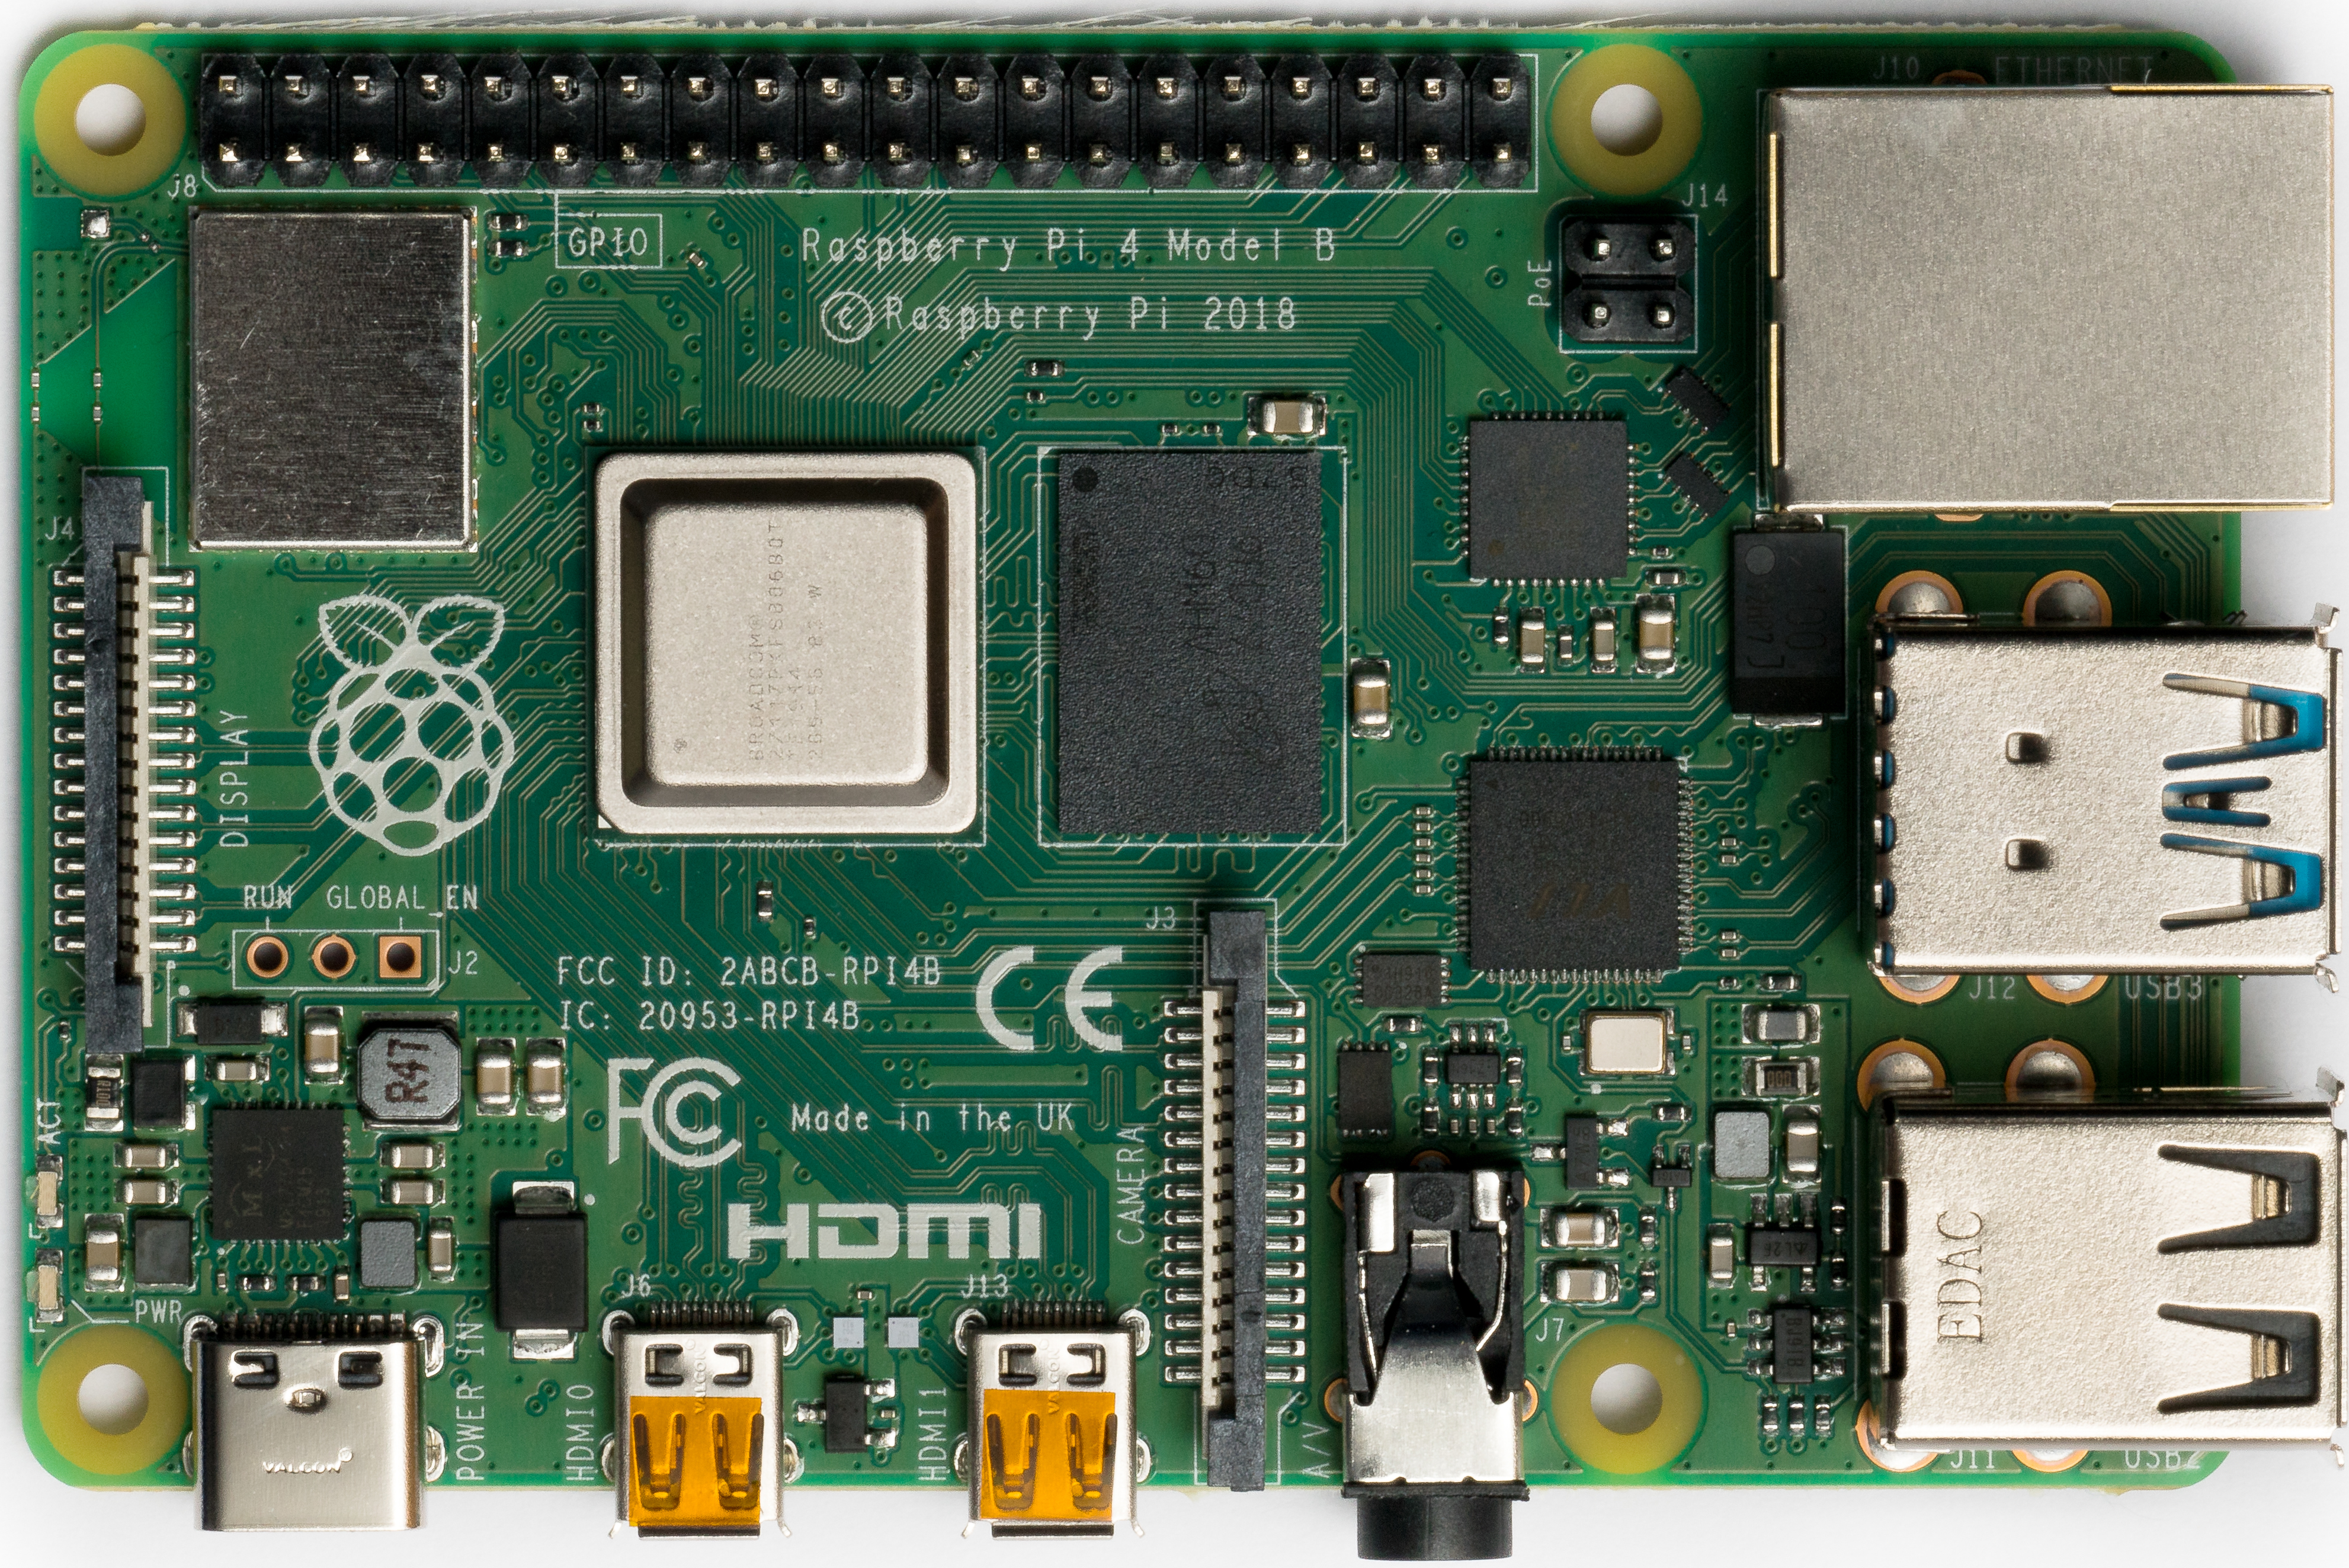
\includegraphics[width=0.22\textwidth,height=2.6cm,keepaspectratio]{figures/photos/03_Raspberry_Pi_4_Model_B.jpg} &
 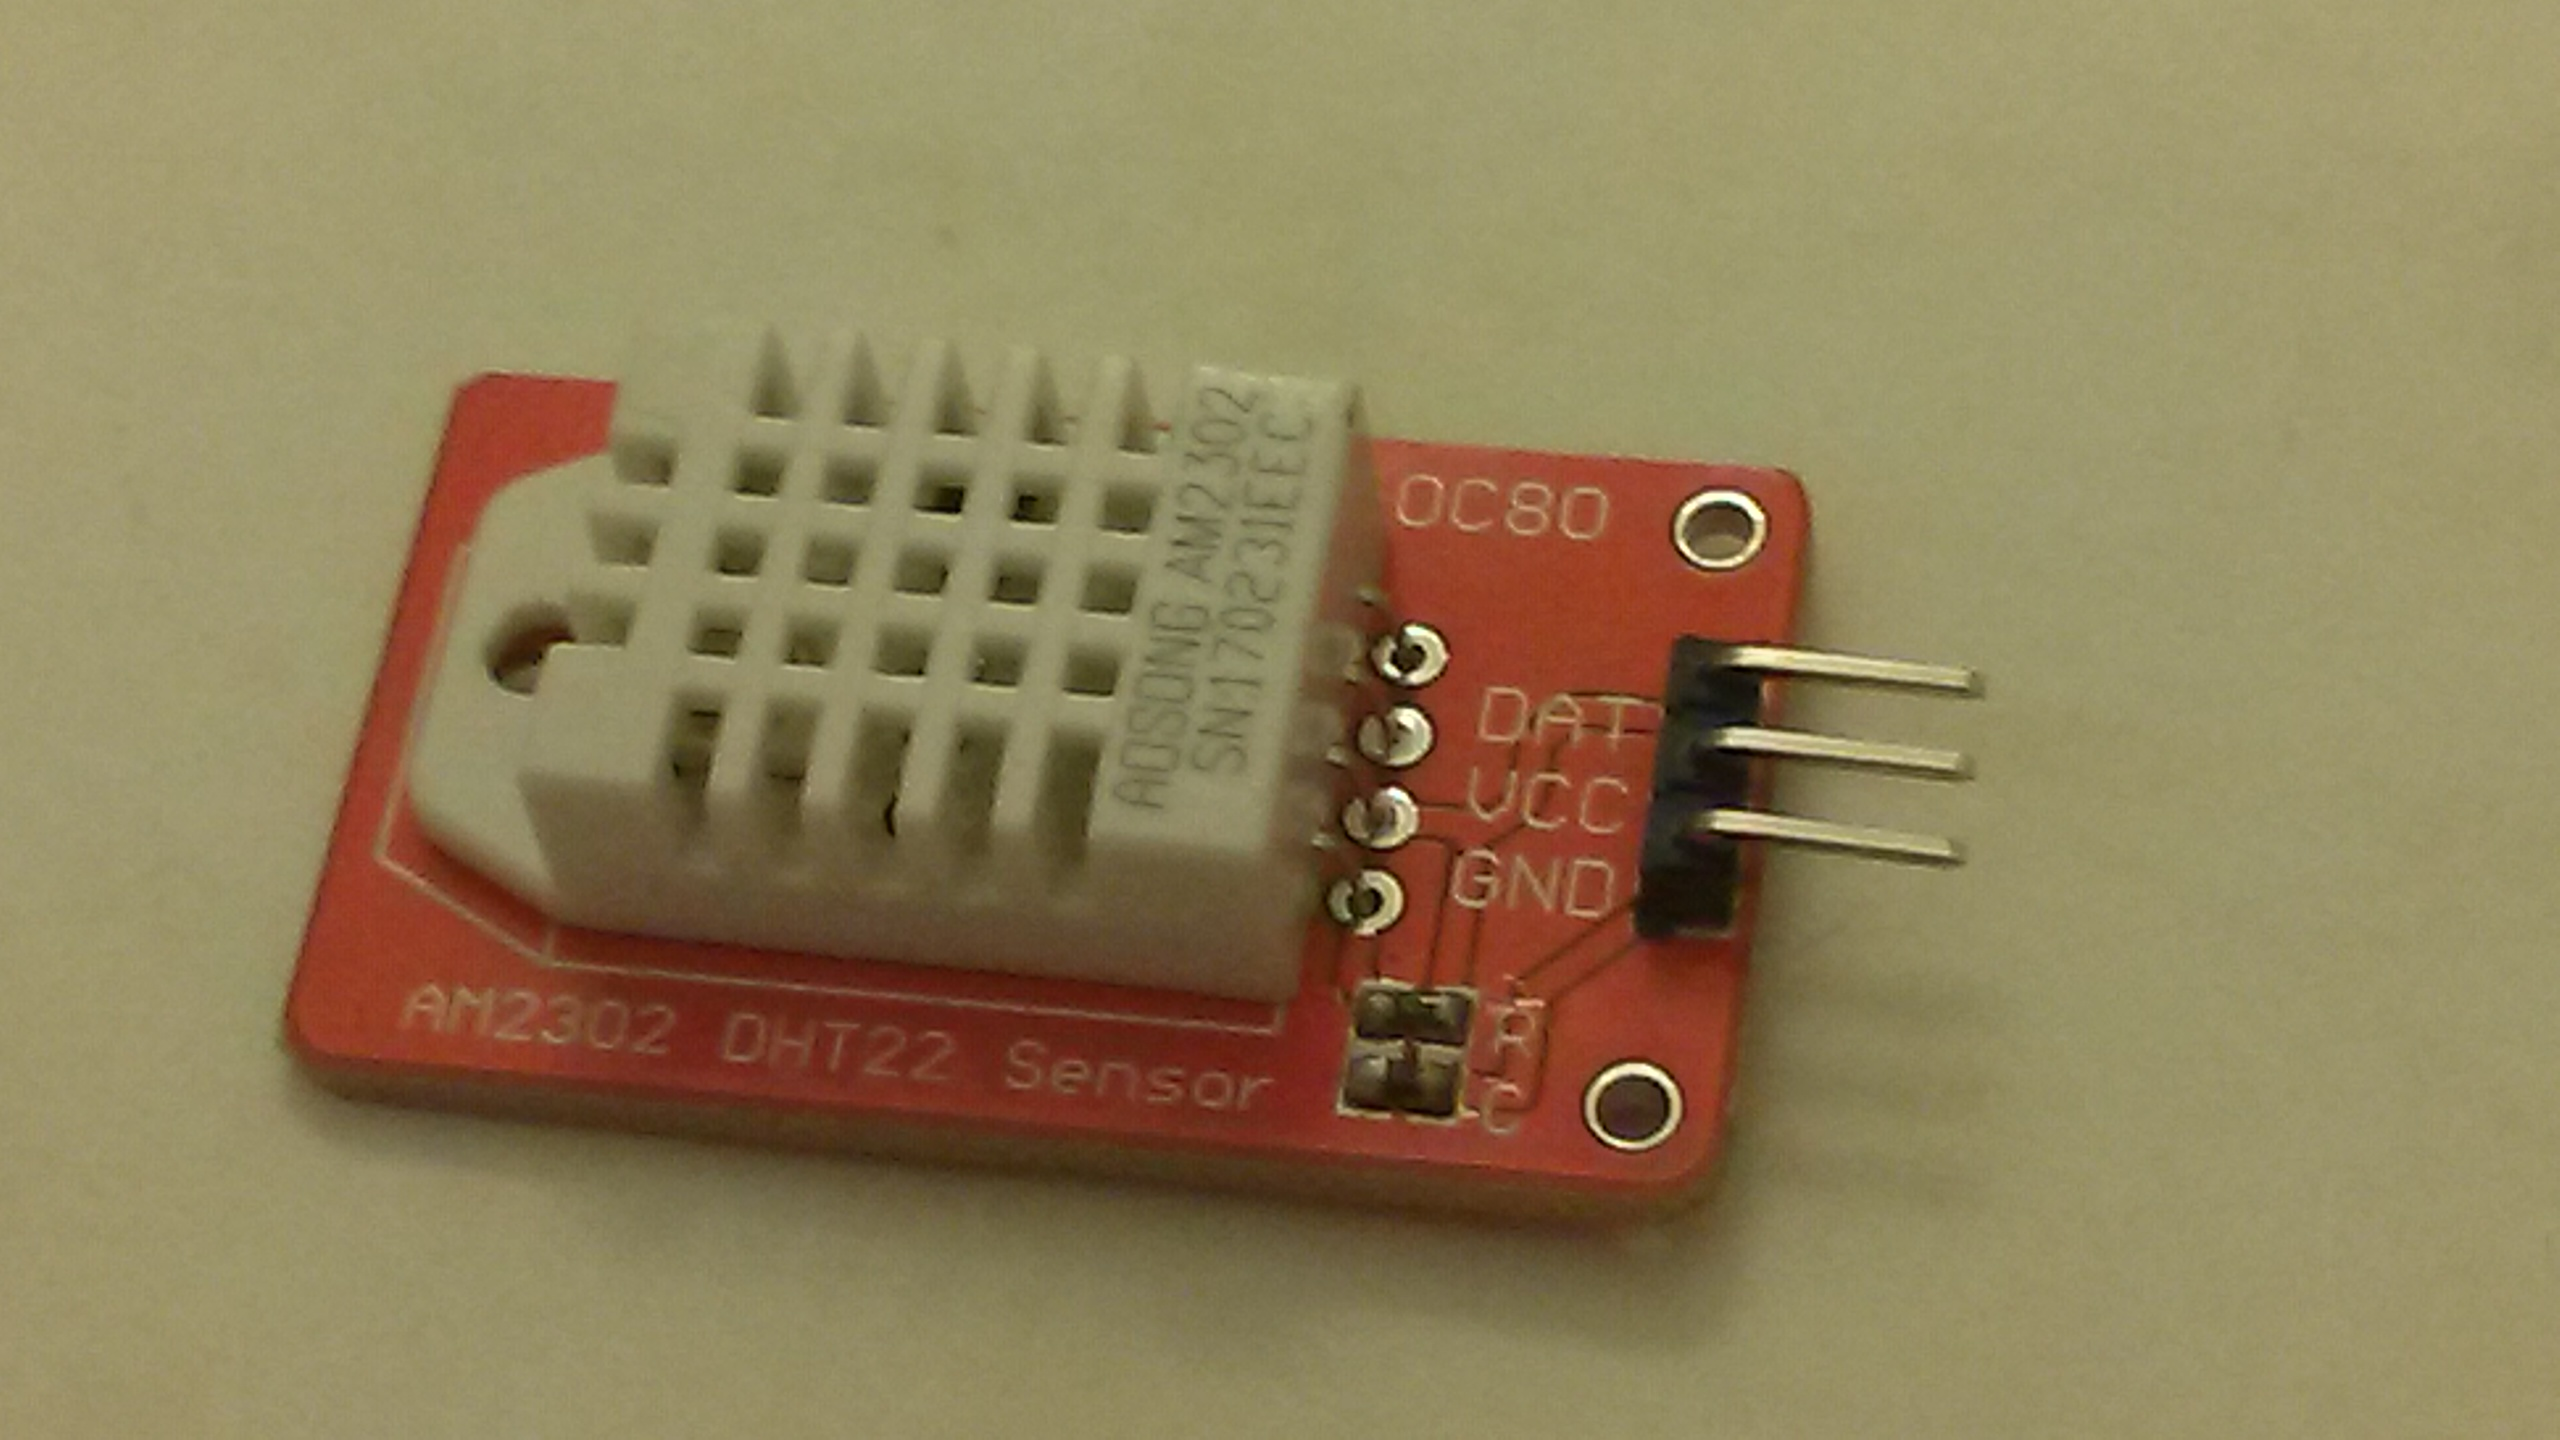
\includegraphics[width=0.22\textwidth,height=2.6cm,keepaspectratio]{figures/photos/01_DHT22_temperature_humidity_sensor.jpg} &
 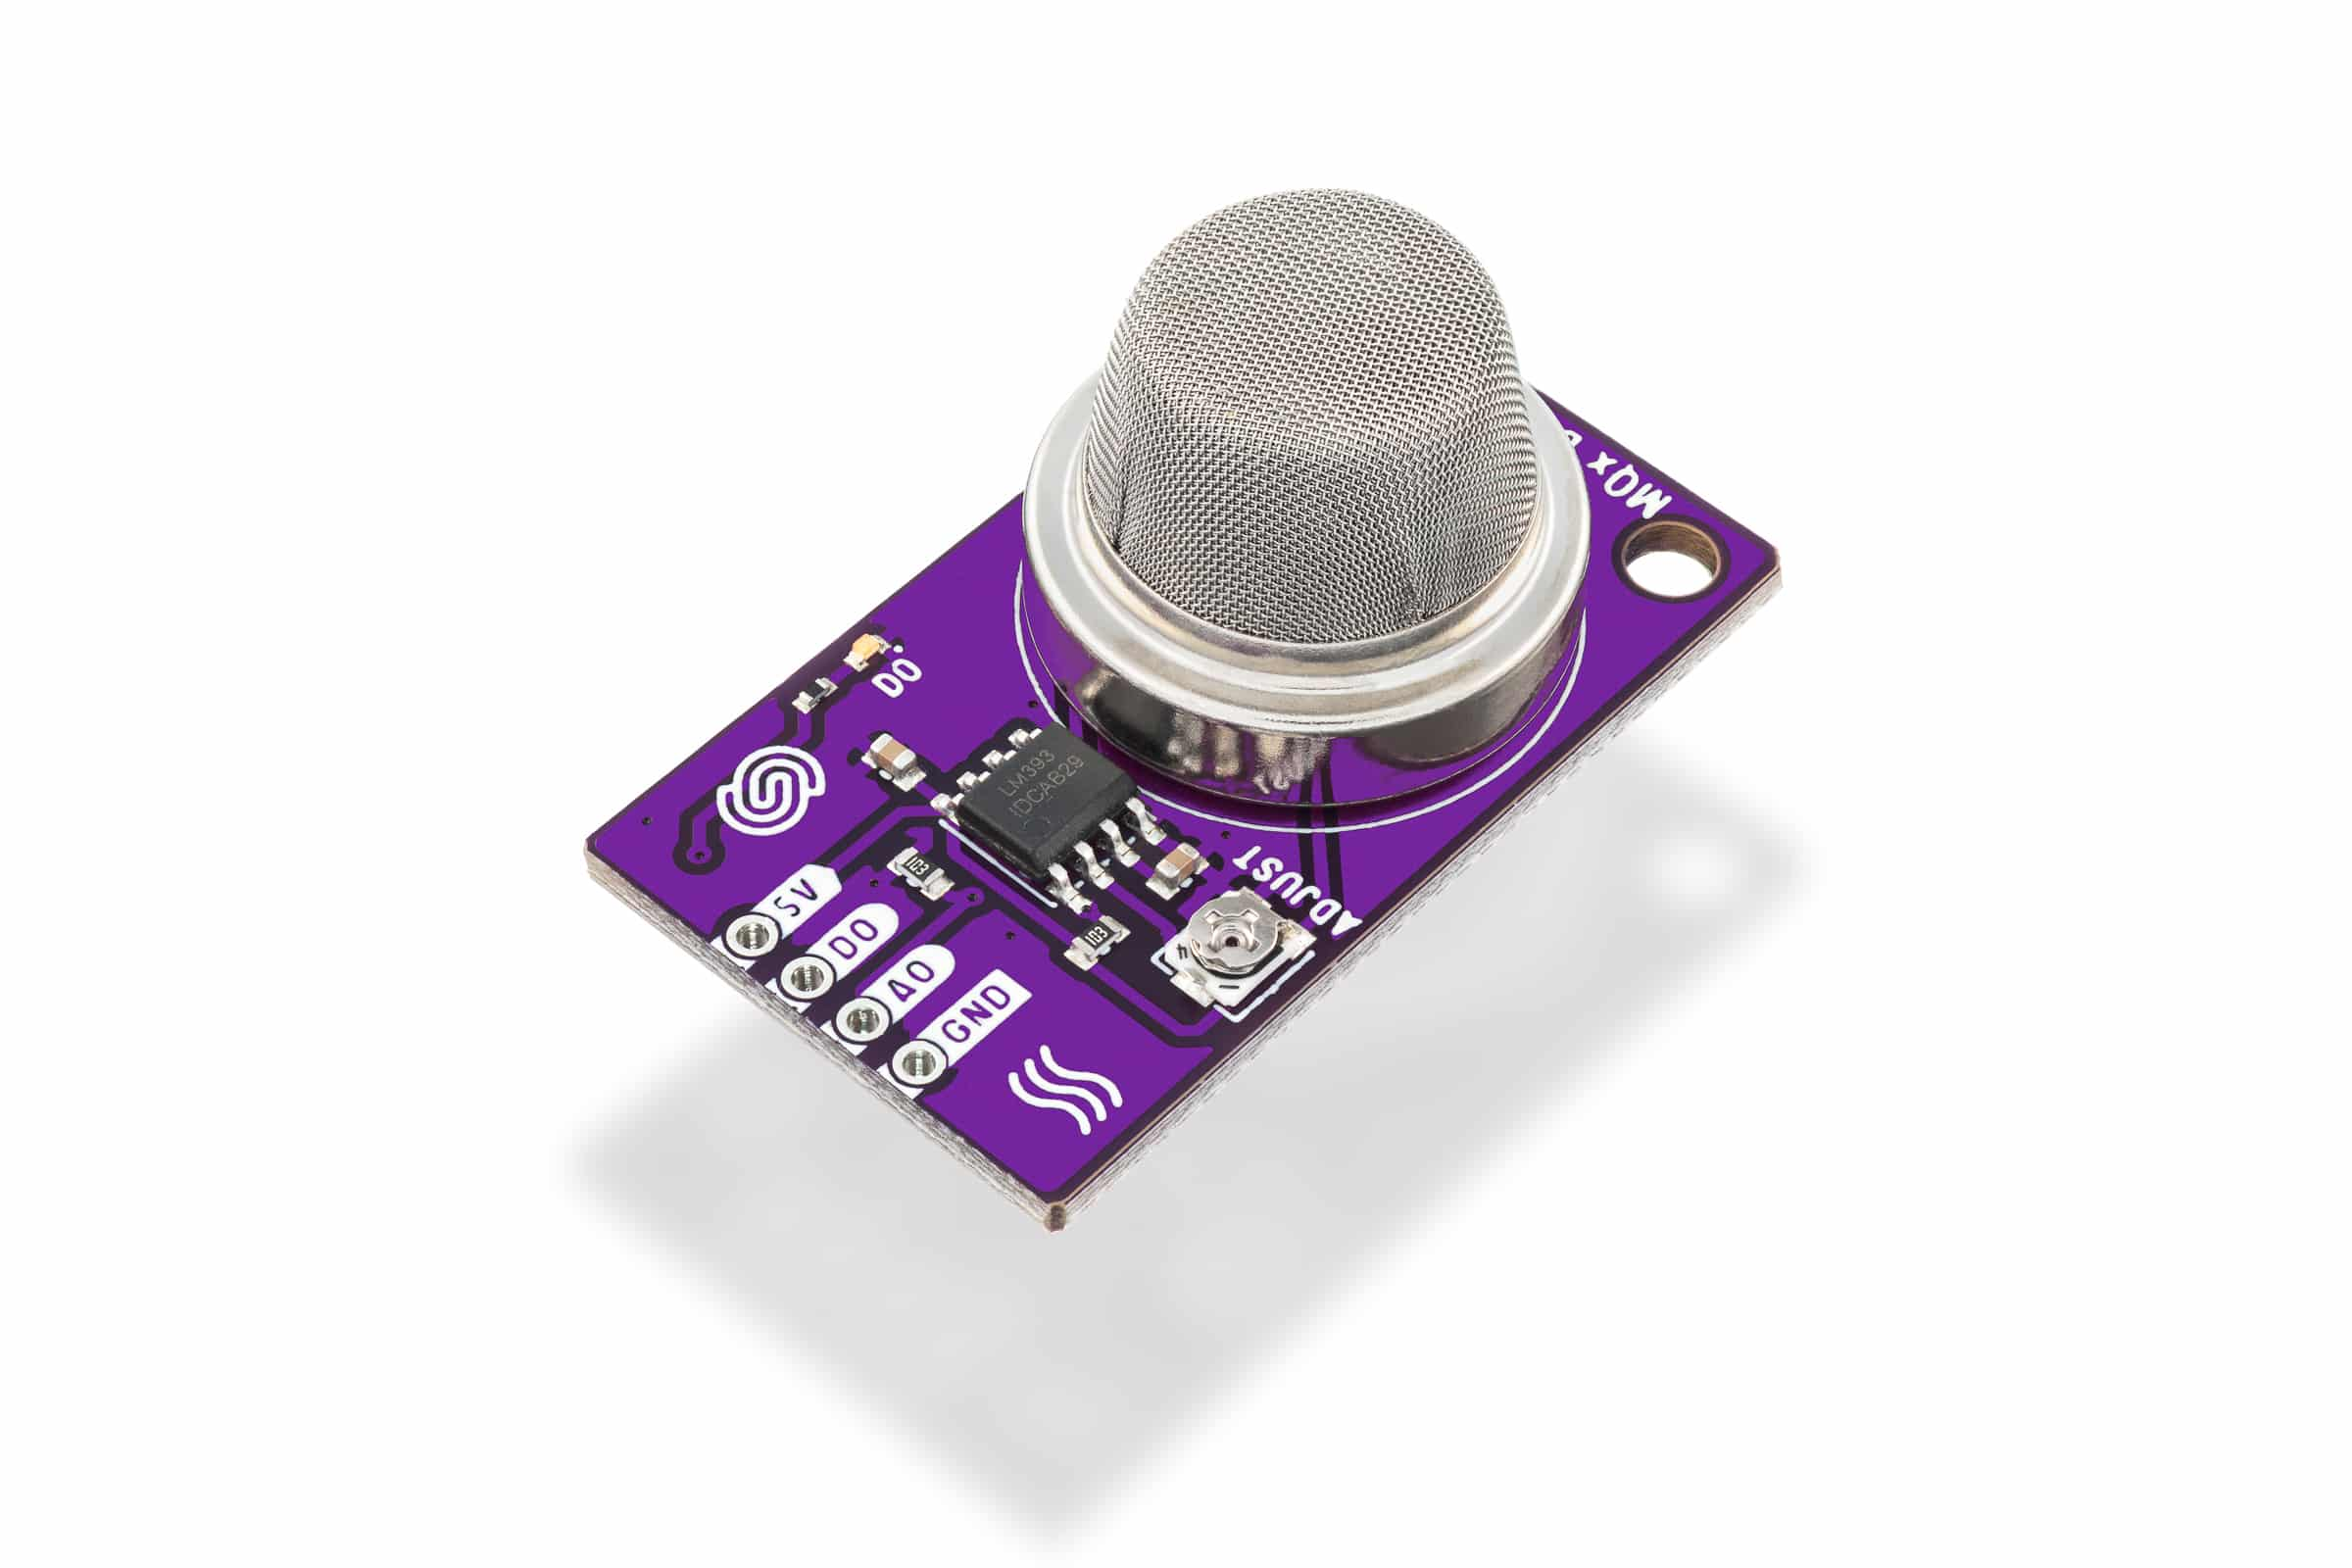
\includegraphics[width=0.22\textwidth,height=2.6cm,keepaspectratio]{figures/photos/02_MQ135_gas_sensor.jpg} &
 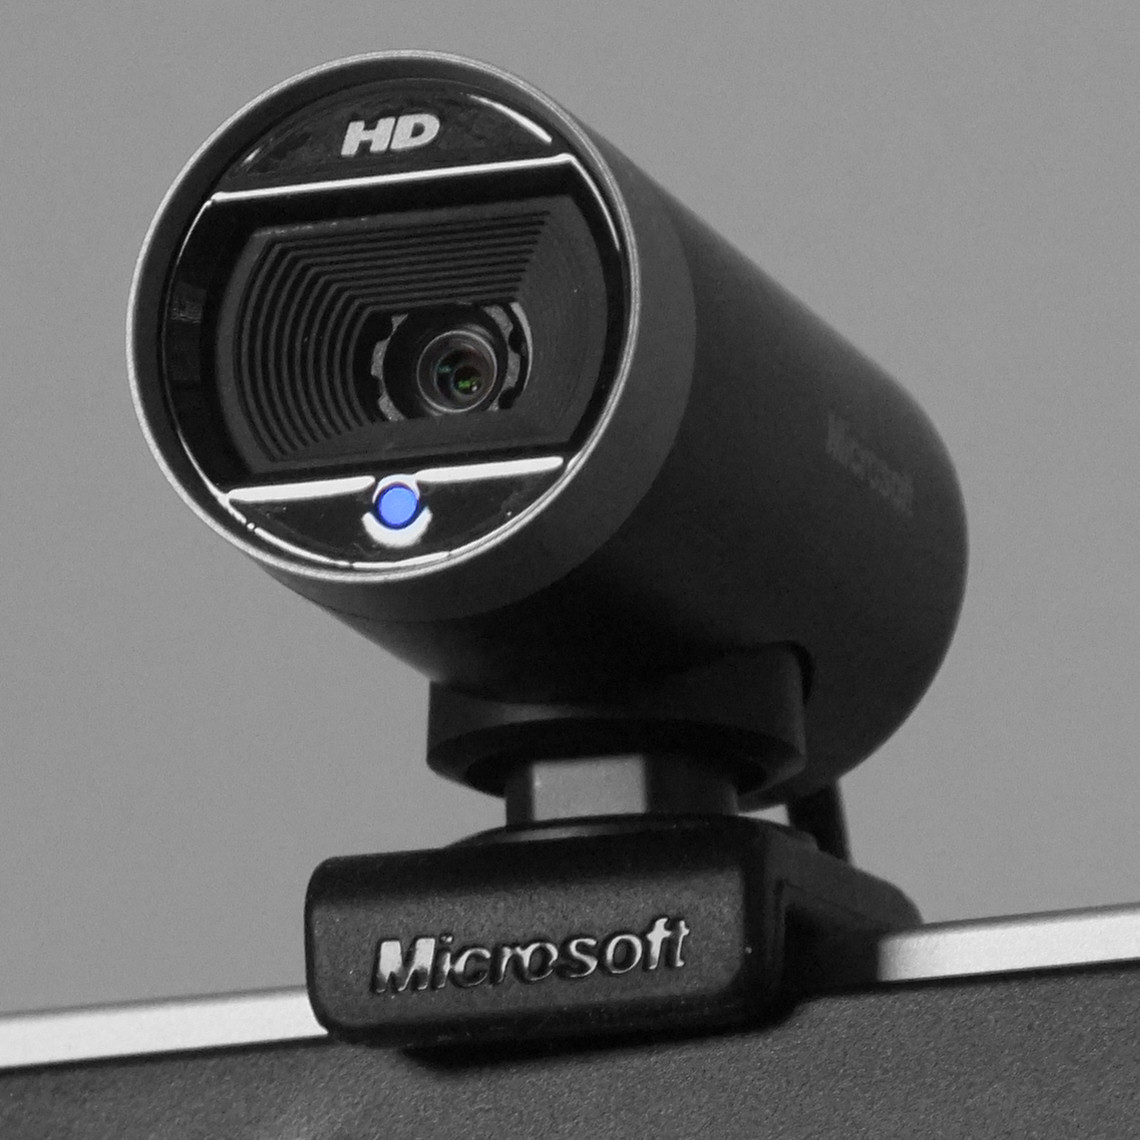
\includegraphics[width=0.22\textwidth,height=2.6cm,keepaspectratio]{figures/photos/04_USB_webcam.jpg} \\
 {\scriptsize Raspberry Pi 4} & {\scriptsize DHT22} & {\scriptsize MQ135 gas sensor} & {\scriptsize USB webcam} \\[4pt]
 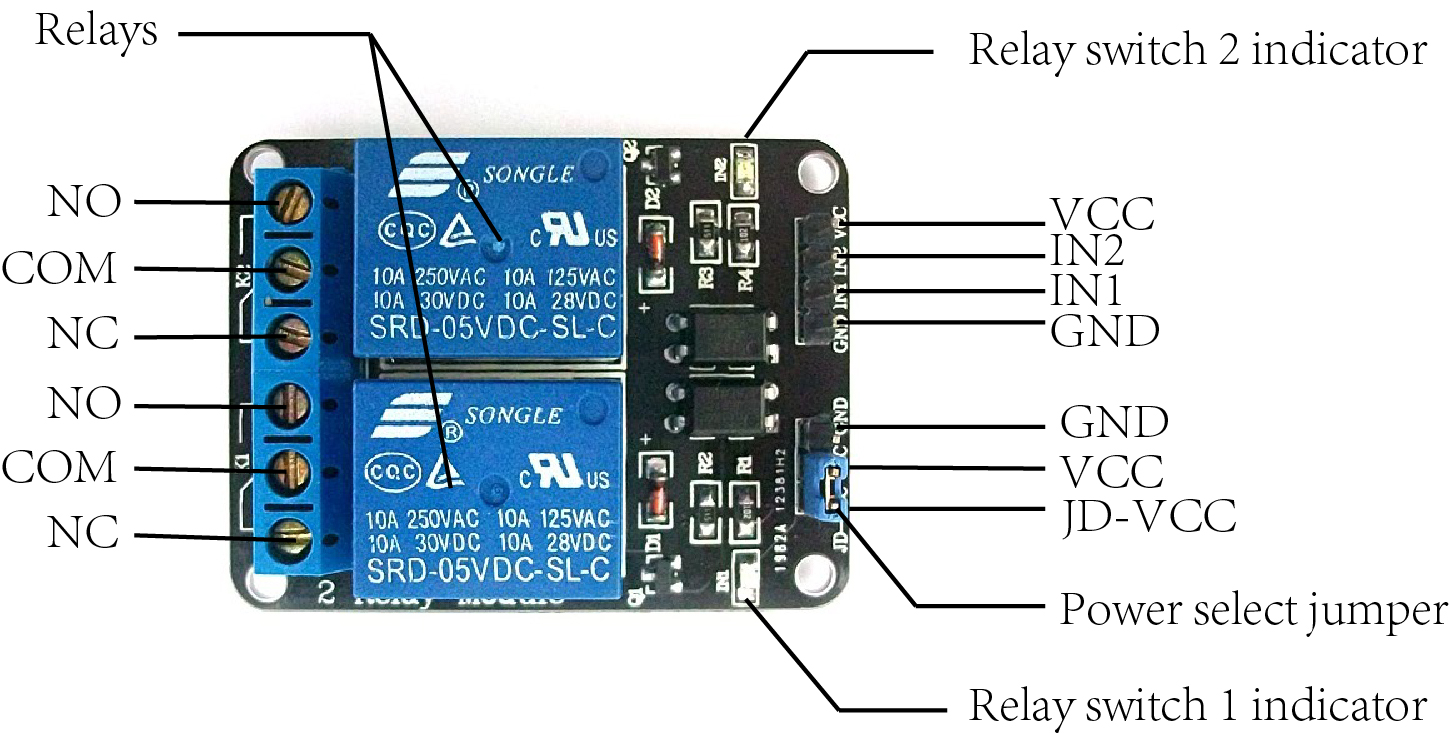
\includegraphics[width=0.22\textwidth,height=2.6cm,keepaspectratio]{figures/photos/05_2_channel_relay_module.jpg} &
 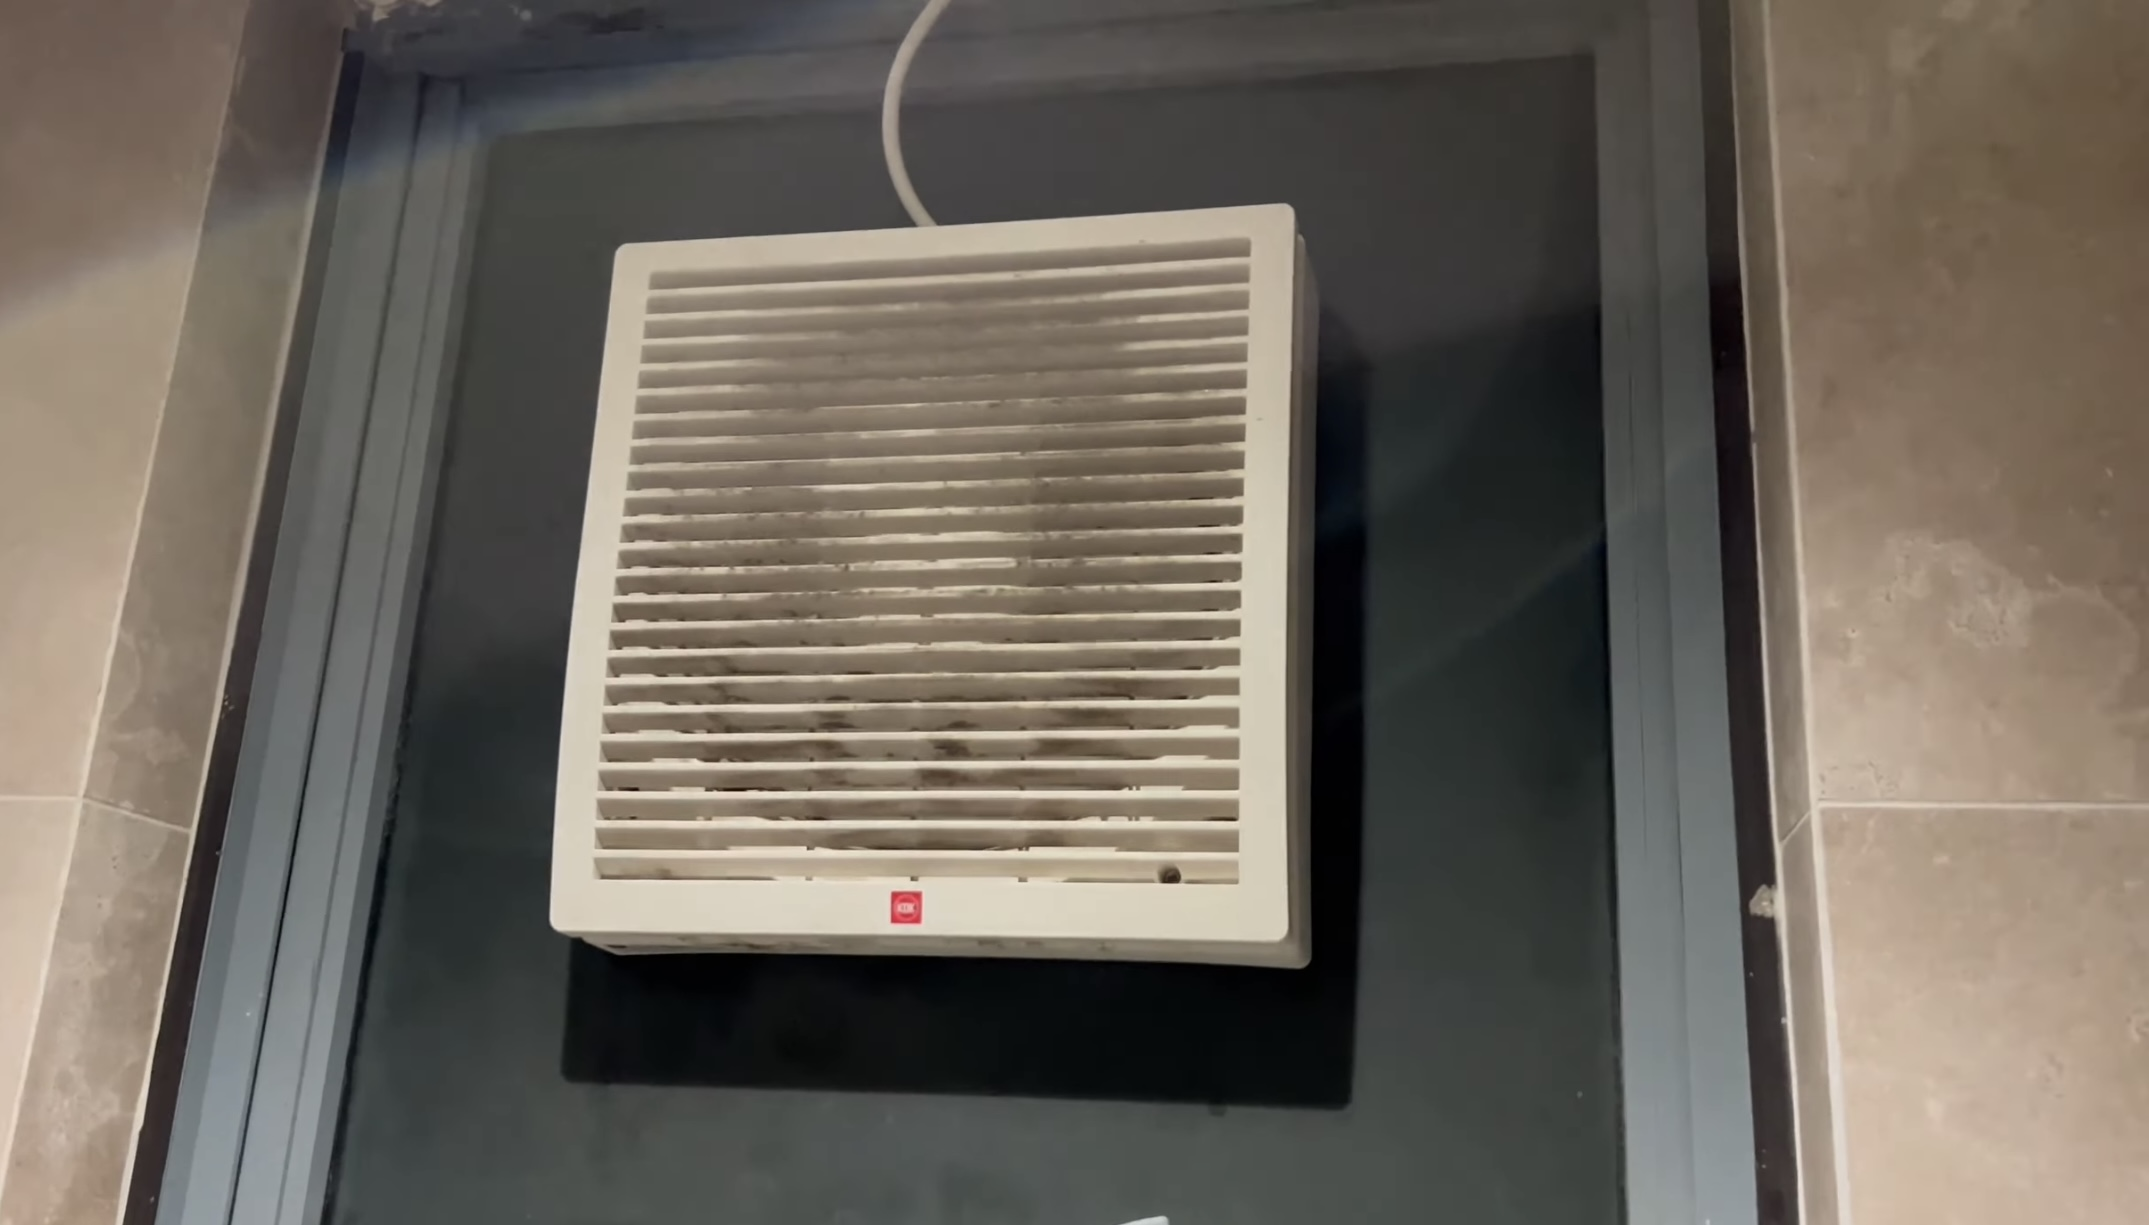
\includegraphics[width=0.22\textwidth,height=2.6cm,keepaspectratio]{figures/photos/06_ventilation_fan.jpg} &
 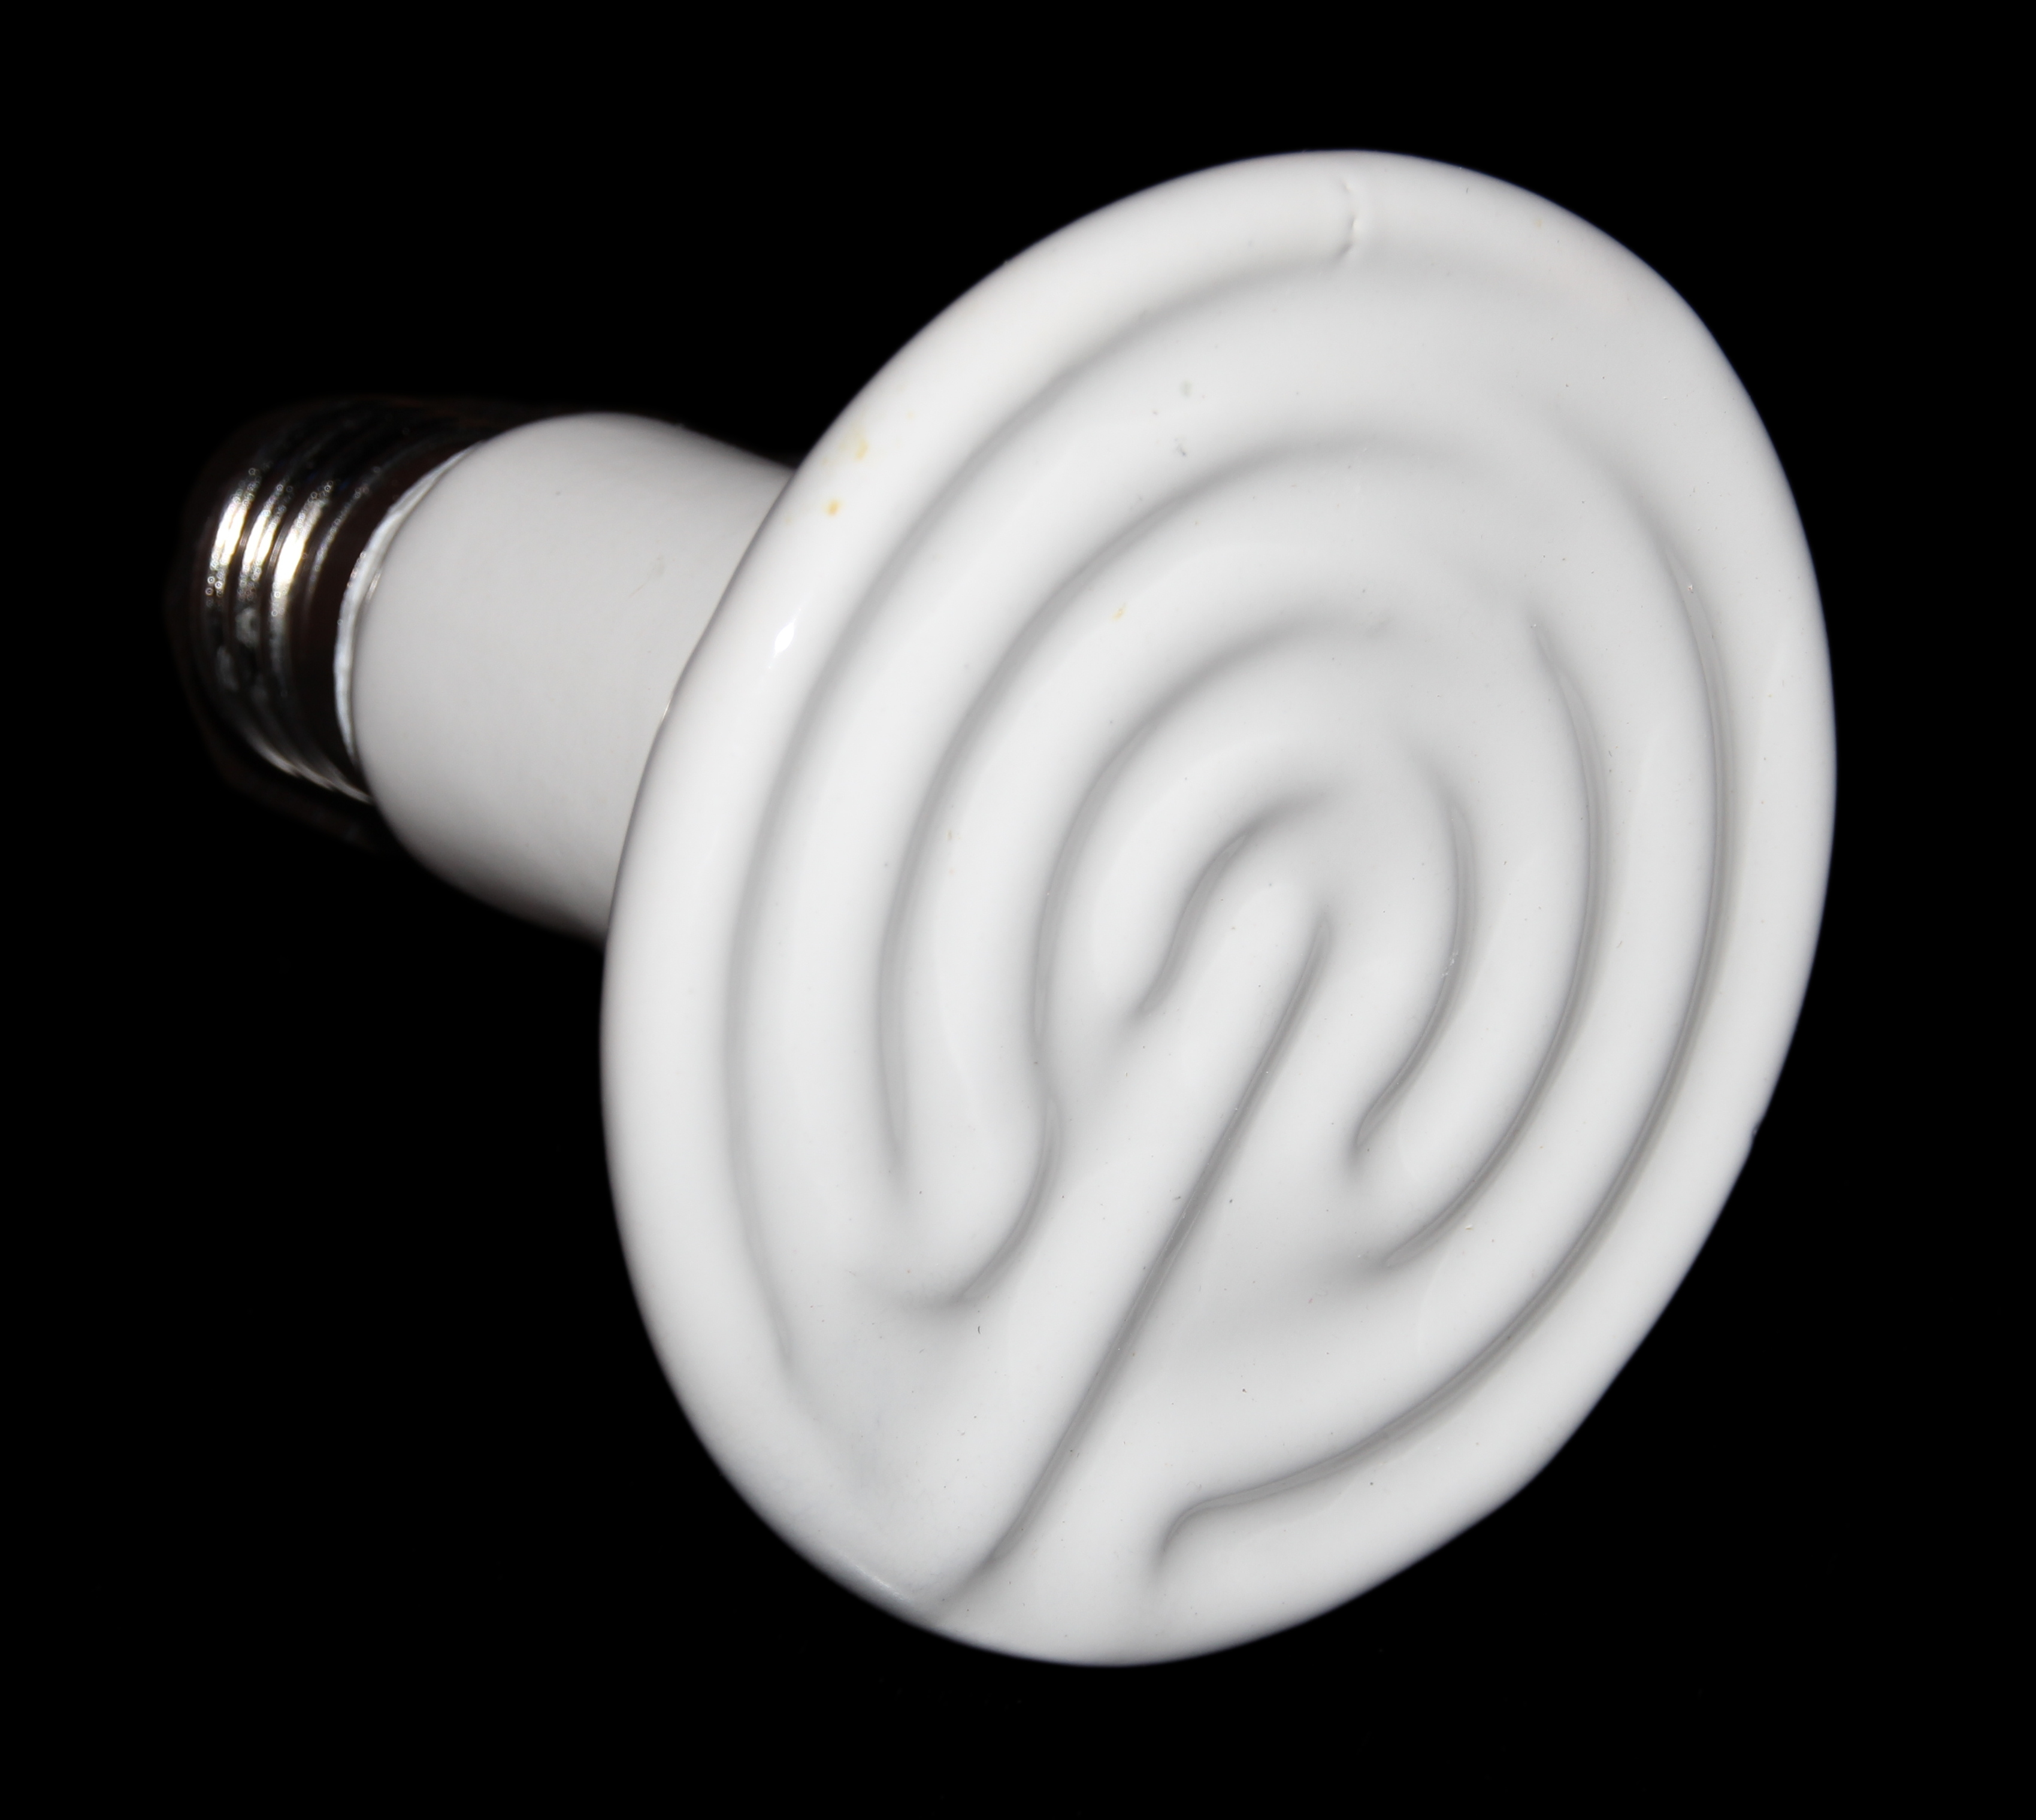
\includegraphics[width=0.22\textwidth,height=2.6cm,keepaspectratio]{figures/photos/07_infrared_heat_lamp.jpg} &
 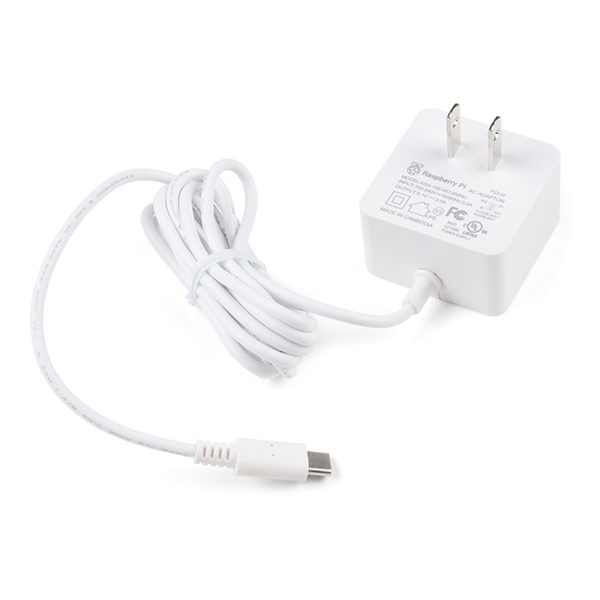
\includegraphics[width=0.22\textwidth,height=2.6cm,keepaspectratio]{figures/photos/08_Raspberry_Pi_5V_power_supply.jpg} \\
 {\scriptsize 2-channel relay} & {\scriptsize Ventilation fan} & {\scriptsize Heat lamp} & {\scriptsize 5\,V power supply} \\
 \end{tabular}
 }{%
 \fbox{\parbox[c][6cm][c]{0.88\textwidth}{\centering\textbf{Component photographs}\\[0.3cm]
 Expected files: \texttt{figures/photos/01--08\_*.jpg}}}%
 }
 \caption{Principal hardware components of the proposed system}
 \label{fig:components}
\end{figure}

\subsection{Machine-Learning Materials}

The machine-learning subsystem is developed using public poultry datasets (the RGB subset of the broiler pathological phenomena dataset associated with Elmessery et al.\ (2023), and the Broiler-Net behaviour material of Zarrat Ehsan and Mohtavipour (2024)) supplemented with locally captured GreenFarms Poultry images and video. Annotation uses standard open-source tools. Model development is conducted in Google Colab using its GPU runtime, in Python with OpenCV for image handling, NumPy and Pandas for data manipulation, Matplotlib for visualisation, and scikit-learn for metrics and data splitting. Detection models use the Ultralytics YOLO implementation; classification, where used, employs EfficientNet or MobileNet via TensorFlow/Keras. Trained models are exported to TensorFlow Lite, ONNX, or NCNN for Raspberry Pi deployment. These materials are listed in Table~\ref{tab:mlmat}.

\begin{table}[tbp]
\caption{Machine-learning materials and tools}
\label{tab:mlmat}
\centering
\small
\begin{tabularx}{\textwidth}{|>{\raggedright\arraybackslash}p{3.3cm}|X|}
\hline
\rowcolor{headerblue}
\textbf{Material/tool} & \textbf{Role} \\
\hline
Public datasets (Elmessery et al., 2023, RGB; Zarrat Ehsan \& Mohtavipour, 2024) & Primary training/reference data for distress and behaviour classes \\
\hline
Local GreenFarms images/video & Domain adaptation and minority-class examples \\
\hline
Annotation tools (open-source) & Bounding-box and class annotation; annotation verification \\
\hline
Google Colab (GPU runtime) & Cloud training environment \\
\hline
Python, OpenCV, NumPy, Pandas, Matplotlib, scikit-learn & Data handling, EDA, metrics, splitting, visualisation \\
\hline
Ultralytics YOLO & Object-detection training and inference \\
\hline
TensorFlow/Keras, EfficientNet/MobileNet & Optional classification stage \\
\hline
TensorFlow Lite / ONNX / NCNN & Model export and quantisation for the Raspberry Pi \\
\hline
\end{tabularx}
\end{table}

\subsection{Software-Development Stack}

The web application is built with Python and Django, exposing a REST API through the Django REST Framework, and backed by PostgreSQL in production (with SQLite used during early development for convenience). The interface uses HTML, CSS, Bootstrap, and JavaScript, with Chart.js for environmental charts. Development uses Git and GitHub for version control, Visual Studio Code as the editor, Postman for API testing, and PlantUML/Graphviz for diagrams. Production deployment uses Gunicorn as the application server behind Nginx, with systemd (or cron for periodic jobs) for process and task management. Only tools actually used in the project are listed; the stack is summarised in Table~\ref{tab:software}.

\begin{table}[tbp]
\caption{Software-development and deployment stack}
\label{tab:software}
\centering
\small
\begin{tabularx}{\textwidth}{|l|X|}
\hline
\rowcolor{headerblue}
\textbf{Tool} & \textbf{Role} \\
\hline
Python, Django, Django REST Framework & Web application and REST API \\
\hline
PostgreSQL (SQLite in early development) & Relational database \\
\hline
HTML, CSS, Bootstrap, JavaScript, Chart.js & Responsive interface and charts \\
\hline
Git, GitHub & Version control \\
\hline
Visual Studio Code, Postman & Development and API testing \\
\hline
PlantUML, Graphviz & Diagram generation \\
\hline
Gunicorn, Nginx, systemd/cron & Deployment and process/task management \\
\hline
\end{tabularx}
\end{table}

\section{Adopted Iterative Development Model}

The system is developed using an iterative development model in preference to the waterfall model \textit{(Royce, 1987)}, which cannot accommodate the emergent requirements of an IoT/AI system, and to full agile frameworks \textit{(Beck et al., 2001)}, which presuppose a multi-person team impractical for a single-researcher project. As \textit{Larman and Basili (2003)} document, iterative and incremental development reduces project risk by validating assumptions early and continuously. The iterative model decomposes the system into increments, each passing through planning, design, build, and test before the next begins, as illustrated in Figure~\ref{fig:iterative}. The model is applied separately to hardware prototyping, dataset preparation, model development, web-application development, subsystem integration, complete-system testing, and optimisation. For each iteration, an objective, inputs, activities, a deliverable, a test, an acceptance criterion, the problem discovered, the feedback obtained, the resulting modification, and an exit criterion are recorded; Table~\ref{tab:iterations} summarises the planned iterations in this form.

\inlinefig{figures/generated/iterative_lifecycle.pdf}{0.58\textwidth}{Iterative development lifecycle with feedback loops}{fig:iterative}

\begin{table}[tbp]
\caption{Planned development iterations (objective, deliverable, test and exit criterion)}
\label{tab:iterations}
\centering
\footnotesize
\renewcommand{\arraystretch}{1.2}
\begin{tabularx}{\textwidth}{|l|X|X|X|}
\hline
\rowcolor{headerblue}
\textbf{Iteration} & \textbf{Objective} & \textbf{Deliverable \& test} & \textbf{Exit criterion} \\
\hline
1. Hardware prototyping & Read DHT22 and gas sensor via ADC; log locally & Breadboard unit; bench test against reference instruments & Stable, plausible readings logged \\
\hline
2. Dataset preparation & Assemble and annotate dataset & Cleaned, split dataset; annotation-verification check & Balanced, leakage-free splits ready \\
\hline
3. Model development & Train detector (and optional classifier) & Trained model; evaluation on held-out test set & Metrics meet target thresholds \\
\hline
4. Web application & Build FMIS and REST API & Django app; unit and API tests & CRUD, auth and API tests pass \\
\hline
5. Integration & Connect edge device to server & End-to-end submission; idempotency test & Records sync without duplication \\
\hline
6. System testing & Validate complete system & Functional and non-functional tests & Requirements satisfied \\
\hline
7. Optimisation & Tune latency, thresholds, usability & Profiled system; operator feedback & Performance and usability targets met \\
\hline
\end{tabularx}
\end{table}

\section{Overall System Workflow}

The end-to-end workflow of the operational system is shown in Figure~\ref{fig:workflow}. Sensors and the camera acquire data; the Raspberry Pi validates and filters inputs, performs inference, evaluates environmental and visual risk, actuates the fan or heater where necessary, and logs records locally; records are transmitted to the Django server through the REST API, validated, and stored in PostgreSQL; dashboards are updated and users are alerted; users acknowledge and resolve alerts, and corrective actions are recorded; and any records buffered during a network outage are synchronised on reconnection. The overall layered architecture is depicted in Figure~\ref{fig:overall}.

\dedicatedfig{figures/generated/system_workflow.pdf}{Complete operational system workflow from sensing to user action}{fig:workflow}
\dedicatedfig{figures/generated/overall_system_architecture.pdf}{Overall layered system architecture}{fig:overall}

\section{Hardware Subsystem Design and Development}

\subsection{Hardware Architecture}

The hardware architecture, shown in Figure~\ref{fig:hwarch}, centres on the Raspberry Pi, which interfaces with the DHT22 over a digital GPIO line, with the gas sensor through an external ADC over SPI or I\textsuperscript{2}C, with the camera over USB or the camera serial interface, and with the fan and heater through an opto-isolated relay module driven from GPIO. A regulated 5\,V supply powers the Pi, while the actuators are switched on the mains side of the relays, physically and electrically separated from the low-voltage logic.

\inlinefig{figures/generated/hardware_architecture.pdf}{0.85\textwidth}{Hardware architecture and component interconnections}{fig:hwarch}

\subsection{Component Selection}

Component selection follows directly from the comparative analysis of Chapter~2 and the requirements of Section~3.4: a single-board computer for on-device vision, a digital DHT22 to avoid an ADC for temperature/humidity, a low-cost metal-oxide gas sensor as a risk indicator, an external ADC to overcome the Pi's lack of analogue input, and opto-isolated relays to switch mains actuators safely. Each selection, together with its justification, limitation, and an alternative, is recorded in Table~\ref{tab:hardware}.

\subsection{Electrical Interface Design}

The electrical interface is designed so that all mains-voltage wiring is confined to the relay output side and the actuators, while the Pi, sensors, and ADC operate at low voltage. The relay module is opto-isolated to prevent mains transients from reaching the Pi. Proposed GPIO assignments are given in Table~\ref{tab:gpio}; these are \emph{proposed and subject to validation} during hardware bring-up, and final pin numbers will be confirmed against the deployed wiring. Pull-up requirements for the DHT22 data line and the SPI/I\textsuperscript{2}C lines for the ADC are observed, and common ground is established between the Pi, the ADC, and the sensors.

\begin{table}[tbp]
\caption{Proposed GPIO assignments (subject to validation during hardware bring-up)}
\label{tab:gpio}
\centering
\small
\begin{tabularx}{\textwidth}{|l|l|X|}
\hline
\rowcolor{headerblue}
\textbf{Signal} & \textbf{Proposed pin/bus} & \textbf{Notes} \\
\hline
DHT22 data & GPIO (1-wire), proposed BCM4 & Requires pull-up resistor \\
\hline
ADC (MCP3008) & SPI0 (MOSI/MISO/SCLK/CE0) & Reads analogue gas sensor \\
\hline
ADC (ADS1115) alternative & I\textsuperscript{2}C (SDA/SCL) & Alternative to MCP3008 \\
\hline
Relay channel 1 (fan) & GPIO, proposed BCM17 & Active-low opto-isolated input \\
\hline
Relay channel 2 (heater) & GPIO, proposed BCM27 & Active-low opto-isolated input \\
\hline
Camera & USB / CSI & Frame capture \\
\hline
\end{tabularx}
\end{table}

The detailed signal-level wiring is specified in Table~\ref{tab:wiring}. The DHT22 data line is connected to a single GPIO pin with a pull-up resistor of about 10\,k$\Omega$ between the data line and the 3.3\,V rail, as required for reliable one-wire signalling; the sensor is powered from the Pi's 3.3\,V supply. The MQ-series gas sensor is powered from 5\,V (its heater requires 5\,V) but its analogue output is scaled to remain within the ADC input range; the analogue output is taken to a single channel of the MCP3008, which communicates with the Pi over the SPI bus (MOSI, MISO, SCLK, and a chip-select line). Where the ADS1115 is used instead, it communicates over the I\textsuperscript{2}C bus (SDA and SCL) and its programmable gain is set so that the sensor's output spans a usable fraction of the converter's full-scale range. A common ground is shared between the Pi, the ADC, the sensors, and the relay logic supply so that all signals are referenced to the same potential.

The relay module is driven from two GPIO pins. The opto-isolated inputs are active-low, so a GPIO is driven low to energise the corresponding relay; the relay logic side is powered from the Pi's 5\,V rail while the relay coil/switching side is, where possible, powered from a separate supply through the module's jumper so that coil switching transients are kept off the Pi's rail. Because the GPIO pins source only only a few milliamperes, the opto-isolator input resistors are sized so that each input draws a current within the safe per-pin limit of the Pi. The fan and the heater are connected to the normally-open relay contacts on the mains side; for the inductive fan load a snubber (or a flyback arrangement appropriate to the contact type) is fitted across the contacts to suppress switching transients. All mains-side conductors are kept physically separated from the low-voltage wiring and are confined within the enclosure.

\begin{table}[tbp]
\caption{Signal-level wiring and connection schedule (proposed, subject to validation)}
\label{tab:wiring}
\centering
\footnotesize
\renewcommand{\arraystretch}{1.2}
\begin{tabularx}{\textwidth}{|l|l|X|}
\hline
\rowcolor{headerblue}
\textbf{From} & \textbf{To} & \textbf{Connection detail} \\
\hline
DHT22 VCC & Pi 3.3\,V & Sensor power \\
\hline
DHT22 DATA & Pi GPIO (1-wire) & 10\,k$\Omega$ pull-up to 3.3\,V \\
\hline
DHT22 GND & Pi GND & Common ground \\
\hline
MQ135 VCC & 5\,V supply & Heater requires 5\,V \\
\hline
MQ135 AOUT & MCP3008 CH0 & Analogue output, scaled to ADC range \\
\hline
MCP3008 VDD/VREF & Pi 3.3\,V & Reference and supply \\
\hline
MCP3008 CLK/DOUT/DIN/CS & Pi SPI (SCLK/MISO/MOSI/CE0) & SPI bus to Pi \\
\hline
MCP3008 AGND/DGND & Pi GND & Common ground \\
\hline
Relay IN1 & Pi GPIO (fan) & Active-low control \\
\hline
Relay IN2 & Pi GPIO (heater) & Active-low control \\
\hline
Relay VCC/GND & Pi 5\,V / GND & Logic-side supply \\
\hline
Fan (mains live) & Relay 1 COM/NO & Switched mains; snubber across contacts \\
\hline
Heater (mains live) & Relay 2 COM/NO & Switched mains; guarded lamp \\
\hline
Camera & Pi USB / CSI & Frame capture \\
\hline
\end{tabularx}
\end{table}

\subsection{Sensor Data Acquisition}

Sensor data acquisition follows the workflow in Figure~\ref{fig:sensoracq}. After initialisation and gas-sensor warm-up, the Pi reads the DHT22 and the ADC at a configurable sampling interval (of the order of tens of seconds to a few minutes). Each reading is timestamped and tagged with a device identifier and a pen identifier, validated, filtered, checked for missing values, appended to a local log, and queued for transmission.

\inlinefig{figures/generated/sensor_acquisition_workflow.pdf}{0.62\textwidth}{Sensor data-acquisition workflow}{fig:sensoracq}

\subsection{Sensor Calibration and Validation}

The DHT22 is validated by comparison against a reference thermometer and hygrometer across the expected operating range, and any systematic offset is recorded for correction. The metal-oxide gas sensor is given a warm-up period before readings are trusted, and a baseline is established in clean air; because the sensor is non-selective, its output is interpreted as a relative risk index rather than an absolute ammonia concentration, and sensor drift over time is acknowledged and periodically re-baselined. Calibration procedures and the reference instruments used are recorded so that the validation can be reproduced. The resulting comparison for the DHT22 is presented in Figure~\ref{fig:calib}. The metal-oxide gas sensor is not calibrated against a reference ammonia concentration, since no such reference was available, and its output is therefore reported throughout as a relative risk index rather than as a measured concentration.

\pendingfig{figures/screenshots/p01_sensor_calibration.png}{7.5cm}{Sensor calibration: DHT22 readings against reference instruments}{fig:calib}

\subsection{Data Filtering and Validation}

Raw readings are validated against plausible physical ranges and subjected to a moving-median filter to suppress transient noise and spikes; values failing the range check trigger a re-read, and isolated outliers are rejected. Missing or corrupt readings are handled by carrying forward the last valid value for a bounded interval and flagging prolonged gaps. This filtering ensures that the threshold logic and the transmitted records are based on stable, plausible data.

\subsection{Environmental Threshold and Hysteresis Logic}

Environmental risk is evaluated against configurable thresholds with three bands, normal, warning, and critical, for temperature, humidity, and gas-risk. Indicative bands, derived from the welfare literature of Chapter~2 and configurable in software, are: temperature safe 18--26\textdegree C (warning 27--30\textdegree C; critical $>$30\textdegree C or $<$18\textdegree C); humidity safe 50--70\% (warning 71--80\%; critical $>$80\% or $<$40\%); and gas-risk index safe below a baseline-relative threshold (warning and critical at progressively higher relative levels). To prevent rapid actuator cycling around a threshold, hysteresis is applied: an actuator switches on at a threshold but switches off only after the parameter has returned past a separate, lower release point. Minimum on-time and minimum off-time constraints further protect the actuators. The control logic is shown in Figure~\ref{fig:ctrl}.

\subsection{Fan and Heater Control}

The fan is engaged when temperature, humidity, or gas-risk indicate the need for increased air exchange or cooling, and the heater is engaged when temperature falls below the safe band, subject to the hysteresis and minimum on/off constraints above. A manual override allows staff to force an actuator on or off, and a fail-safe policy defines safe default states (for example, defaulting to ventilation on loss of a reliable temperature reading, and never leaving the heater energised without a valid low-temperature signal). The pseudocode below summarises the per-cycle control and alerting logic.

\noindent\begin{minipage}{\linewidth}
\begin{lstlisting}[style=pseudocode]
FUNCTION controlCycle(temp, humidity, gasRisk):
    level = "NORMAL"
    IF temp > T_CRIT_HI OR temp < T_CRIT_LO OR
       humidity > H_CRIT_HI OR humidity < H_CRIT_LO OR
       gasRisk > G_CRIT THEN
        level = "CRITICAL"
    ELSE IF temp > T_WARN OR humidity > H_WARN OR
            gasRisk > G_WARN THEN
        level = "WARNING"
    END IF
    // Actuation with hysteresis and min on/off enforcement
    IF temp >= T_FAN_ON THEN requestFan(ON)
    ELSE IF temp <= T_FAN_OFF THEN requestFan(OFF)
    IF temp <= T_HEAT_ON THEN requestHeater(ON)
    ELSE IF temp >= T_HEAT_OFF THEN requestHeater(OFF)
    applyMinOnOff(fan); applyMinOnOff(heater)
    IF level != "NORMAL" THEN raiseAlert(level, parameter, value)
    logState(temp, humidity, gasRisk, level, fan, heater, timestamp)
    bufferAndQueue(record)
END FUNCTION
\end{lstlisting}
\end{minipage}

\inlinefig{figures/generated/environmental_control_algorithm.pdf}{0.7\textwidth}{Environmental-control decision logic with warning/critical bands}{fig:ctrl}

\subsection{Power Budget and Supply}

The Raspberry Pi is supplied from a regulated 5\,V source rated for the peak current of the board and its USB peripherals (a 5\,V/3\,A supply for a Raspberry Pi 4, and a higher-rated USB-C supply for a Raspberry Pi 5). The sensors and the ADC draw negligible current from the Pi's 3.3\,V and 5\,V rails. The actuators are mains-powered and are not drawn from the Pi supply; only the relay logic side is powered from the Pi's 5\,V rail. Where mains supply is unreliable, an uninterruptible supply or battery backup for the Pi is recommended so that sensing, control, and local buffering continue through brief outages; this is noted as an operational provision rather than a core component. A separate, clearly rated supply path for the heat lamp is provided because of its comparatively high power draw.

\subsection{Build and Assembly Procedure}

The unit is built in three stages, consistent with the iterative model. In the first stage, the circuit is assembled on a breadboard for rapid validation: the DHT22, the gas sensor, and the ADC are wired to the Pi as specified in Table~\ref{tab:wiring}, the relay module is connected to two GPIO pins with the actuators initially replaced by indicator loads (for example LEDs) so that switching can be verified safely before any mains load is connected, and each subsystem is tested in isolation. In the second stage, once the wiring is confirmed, the connections are transferred to a soldered prototype board (perfboard) or a simple printed circuit board to remove the unreliability of breadboard contacts, and screw terminals are used for the sensor leads and the relay-to-actuator wiring so that the unit can be serviced. In the third stage, the assembled board, the Pi, and the relay module are mounted inside a protective enclosure fitted with cable glands; the mains wiring to the fan and heater is terminated within the enclosure behind the fuse and circuit breaker, and the low-voltage and mains compartments are kept separated. The camera is mounted to view the birds at an appropriate height and angle for consistent framing, and the DHT22 and gas sensor are positioned at bird level, away from direct draughts from the fan, so that the readings reflect the conditions the birds actually experience. Each build stage concludes with a bring-up test: power-on checks, confirmation of plausible sensor readings against the reference instruments, and verification of relay switching and of the fail-safe default states before the unit is left to operate.

\subsection{Iterative Hardware Development}

Hardware development proceeds iteratively (Iteration~1 of Table~\ref{tab:iterations}): a breadboard prototype is built and bench-tested against reference instruments; problems such as wiring faults or noisy readings are diagnosed and corrected; the design is then consolidated onto a more robust interconnection and housed in a protective enclosure; and finally the unit is installed in the poultry house for field validation. Photographic evidence of the breadboard prototype and of the unit installed in the poultry house was obtained and appears as Figures~\ref{fig:breadboard} and \ref{fig:installed}. The consolidation of the design onto a soldered interconnection and into a protective enclosure, and the bench comparison against reference instruments, were not reached within the prototype window.

\pendingfig{figures/photos/p02_breadboard_prototype.jpg}{9cm}{Breadboard prototype of the hardware unit}{fig:breadboard}
\pendingfig{figures/photos/p03_installed_prototype.jpg}{10cm}{Prototype installed in the poultry house}{fig:installed}

\section{Machine-Learning Subsystem Development}

\subsection{Definition of the Machine-Learning Task}

The machine-learning task is defined as a two-stage pipeline: object detection to locate individual birds within each frame, followed, where justified, by image classification of cropped birds into the project-facing visible-risk labels. Detection is required because multiple birds appear in a frame and must be located individually; classification of crops can sharpen the distinction between visually similar conditions. Where a whole-frame behavioural cue such as huddling is the target, frame-level classification is used instead. This decomposition follows the detection-then-analysis architecture that Chapter~2 identified as dominant across the poultry computer-vision literature \textit{(Okinda et al., 2020; Zarrat Ehsan \& Mohtavipour, 2024; Li, 2025)}, and it is adopted here for a concrete engineering reason as much as a methodological one: separating localisation from labelling allows the computationally heavier detector to run at a reduced frame rate while the lighter classifier is invoked only on the crops it produces, keeping the whole pipeline within the latency budget of the Raspberry Pi. The task is framed explicitly as recognising \emph{visible risk} rather than diagnosing disease, so its output is a flag with an associated confidence and, for ambiguous cases, an \texttt{uncertain} label that routes the frame to human review rather than to automatic action. The development pipeline is shown in Figure~\ref{fig:mlpipe} and the on-device inference flow in Figure~\ref{fig:mlinf}.

\dedicatedfig{figures/generated/ml_pipeline.pdf}{Machine-learning development pipeline from data acquisition to model export}{fig:mlpipe}

\subsection{Dataset Acquisition}

Public datasets are acquired from their original repositories, and their licences, quantities, class definitions, and file formats are verified against the source publications before use, and no claims about dataset size or composition are made beyond those stated by the sources. In this study that verification step materially changed the data that could actually be used, and the change is recorded here rather than concealed. The design committed the training work to the RGB subset of the broiler pathological-phenomena dataset \textit{(Elmessery et al., 2023)}, listed among the machine-learning materials of Table~\ref{tab:mlmat}, together with the six-class visible-condition label set (\texttt{healthy}, \texttt{lethargic}, \texttt{open\_beak\_stress}, \texttt{diseased\_eye}, \texttt{slipped\_tendon}, and \texttt{pendulous\_crop}). That subset proved not to be retrievable: the Mendeley record linked from the publication carries only the six hundred thermal images, and the RGB subset is not clearly published there. Because the deployed system senses through a standard RGB webcam, the thermal material is not a usable substitute for it, and the six-class label set was therefore not trainable.

Two substitutions were made in consequence, both from sources whose licences permit research use and whose provenance was recorded with the imported data. The detection stage was trained on the Broiler-Net material \textit{(Zarrat Ehsan \& Mohtavipour, 2024)}, obtained from the authors' official repository under the Apache-2.0 licence, which supplies a single annotated object class, \texttt{chicken}. The classification stage was trained on the \texttt{broiler-chicken-healthy-and-sick} collection published on Roboflow Universe under the CC~BY~4.0 licence, comprising 505 images in the two classes \texttt{Healthy} and \texttt{Sick}. Verification of that second export also established that it distributes three augmented versions of each source image, a horizontal flip, a rotation of plus or minus fifteen degrees, and a brightness change of plus or minus twenty-five per cent, across its own splits, so that transformed copies of a single photograph appear in more than one split as supplied. That defect is corrected before training by applying the leakage-safe splitting principle of Section~3.9.8 at the level of the source image rather than the video segment.

The consequence of the substitution bounds every model result reported in Chapter~4 and is stated plainly. The trained system demonstrates the two-stage pipeline at two health classes, healthy and sick, and not at the six visible-condition classes of the original design; the detector likewise localises birds as a single class rather than distinguishing conditions at the point of detection. The class-to-risk mapping that links the model to the web application remains implemented and tested across the full six-class set, but in this dissertation it is exercised by those tests alone and not by any trained model.

\subsection{Local Data Collection}

Local images and video are collected at GreenFarms Poultry using the deployment camera and viewpoint, capturing the local lighting, bird density, age, breed, background, and litter conditions, so as to address the domain shift and class imbalance identified in Chapter~2. Video is recorded and individual frames are later extracted for annotation. This collection was not accomplished within the prototype window: the edge unit was installed and photographed at GreenFarms Poultry, as Figure~\ref{fig:installed} shows, but no annotated local imagery was assembled, and the models reported in Chapter~4 are therefore trained wholly on the public datasets identified in Section~3.9.2. Local collection consequently remains the primary route by which the trained system would be adapted to the deployment site.

\subsection{Image and Video Annotation}

Frames are annotated with bounding boxes and the project-facing class labels; where classification crops are used, image-level labels are applied. A verification pass re-checks a sample of annotations for consistency, with particular attention to borderline cases (for example, distinguishing a resting bird from a lethargic one), since inconsistent labelling caps achievable accuracy.

\subsection{Exploratory Data Analysis}

Exploratory data analysis characterises the assembled dataset before training: class distribution (to quantify imbalance), image-size distribution, bounding-box size and aspect-ratio distribution, and the prevalence of blur, occlusion, variable lighting, and high bird density. The findings guide augmentation and splitting decisions. The analysis was carried out on the detection material described in Section~3.9.2 and its outputs are reproduced in Figures~\ref{fig:classdist} and \ref{fig:bboxdist}. It recorded 3{,}211 annotated birds across twenty frames drawn from nine video segments, all belonging to the single detection class \texttt{chicken}, which after tiling supplied 3{,}829 training and 974 validation instances. The bounding-box statistics gave a median box size, taken as $\sqrt{wh}$, of 56 pixels and a median aspect ratio $w/h$ of 0.92 within the 1080p source frames. The birds are therefore small and close to square, each occupying only a small part of a full-resolution frame, which is why the frames are tiled rather than presented whole: downscaling an entire 1080p frame to the input resolution of the detector would reduce targets of this size below the scale at which they can reliably be found.

\pendingfig{figures/screenshots/p04_class_distribution.png}{7cm}{Dataset class-distribution chart}{fig:classdist}
\pendingfig{figures/screenshots/p05_bbox_distribution.png}{7cm}{Bounding-box size and aspect-ratio distribution}{fig:bboxdist}

\subsection{Data Cleaning}

Duplicate frames (common when extracting from video) and corrupt or unreadable images are removed, and near-duplicate consecutive frames are pruned to reduce redundancy and the risk of leakage between splits.

\subsection{Data Augmentation}

To mitigate class imbalance and improve robustness to field conditions, augmentation is applied, including horizontal flipping, brightness and contrast variation, mild rotation and scaling, and noise, targeted preferentially at the welfare-critical minority classes. Augmentation is applied only to the training split.

\subsection{Dataset Splitting}

The dataset is split into training, validation, and test subsets. To prevent data leakage, frames originating from the same video segment are kept within a single split, so that near-identical consecutive frames cannot appear in both training and test sets and inflate apparent performance. Stratification preserves class proportions across splits as far as imbalance permits.

\subsection{Selection of the Pretrained Model}

A pretrained model is selected as the starting point for transfer learning. A YOLO detector (via the Ultralytics implementation) is the preferred detection model owing to its real-time performance and suitability for locating multiple birds; EfficientNet or MobileNet is selected for the optional classification stage owing to its accuracy-to-size efficiency on resource-constrained devices. Selection criteria include detection/classification accuracy, model size, and inference speed on ARM hardware.

\subsection{Google Colab Training Environment}

A Google Colab environment was prepared as the intended training platform, since its GPU runtime offers acceleration for transfer learning without local GPU hardware, and the project training notebook was loaded into it with its transfer-learning, evaluation, and Raspberry~Pi export cells in place; that session is shown in Figure~\ref{fig:colab}, and the environment, dependencies, and runtime are recorded for reproducibility. The status of that environment must, however, be stated precisely, because the figure is easily over-read. The cells visible in it are unexecuted, carrying empty prompts and no outputs, and the training call they contain specifies sixty epochs, whereas the run that produced the results reported in Section~4.1 completed forty epochs and was executed on a central processing unit rather than on the Colab GPU. The GPU path is therefore configured and available, and it is the route by which this work would be repeated or extended, but it is not the source of any metric reported in this dissertation, and no claim of GPU-accelerated training is made for those results.

\pendingfig{figures/screenshots/p06_colab_environment.png}{8.5cm}{The Google Colab training environment with the project notebook loaded}{fig:colab}

\subsection{Transfer Learning}

Transfer learning adapts the pretrained model to the poultry task by initialising from pretrained weights and fine-tuning on the assembled dataset, which is far smaller than the datasets on which the base models were originally trained. This reduces data and compute requirements and improves convergence relative to training from scratch.

\subsection{Iterative Model Training}

Model training proceeds iteratively (Iteration~3 of Table~\ref{tab:iterations}): a baseline is trained and evaluated, weaknesses are diagnosed from the validation metrics and error cases, and the data, augmentation, or hyperparameters are adjusted before retraining. Checkpoints are saved and experiments are logged so that configurations and outcomes are traceable.

\subsection{Hyperparameter Tuning}

Hyperparameters tuned include batch size, input image size, learning rate, number of epochs, and optimiser choice, with early stopping used to halt training when validation performance ceases to improve, guarding against overfitting. The confidence threshold for detections is optimised separately against the operating-point requirements (favouring recall of welfare-critical classes while controlling false alerts).

\subsection{Model Evaluation}

Models are evaluated on the held-out test set using the metrics defined in Section~3.15, with classification metrics applied to the classification stage and detection metrics (IoU, mAP) applied to the detector. Error analysis examines false positives and false negatives, since their operational costs differ: a false negative is a missed distress signal, while a false positive risks alert fatigue. The evaluation artefacts specified by this procedure were produced by executing the evaluation stage on the trained models, and they appear as the training and validation loss curves of Figure~\ref{fig:losscurve}, the precision--recall curve of the detector in Figure~\ref{fig:prcurve}, and the confusion matrix of the classification stage in Figure~\ref{fig:confmat}. The values that these artefacts summarise, together with the qualifications that must accompany them, are reported in Section~4.1, since the present section defines the evaluation procedure rather than its outcome.

\pendingfig{figures/screenshots/p07_training_curves.png}{6cm}{Training and validation loss curves}{fig:losscurve}
\pendingfig{figures/screenshots/p08_pr_curve.png}{9cm}{Precision--recall curve of the detection model}{fig:prcurve}
\pendingfig{figures/screenshots/p09_confusion_matrix.png}{8cm}{Confusion matrix of the classification stage}{fig:confmat}

\subsection{Model Export and Raspberry Pi Deployment}

The trained model is exported to an efficient inference format (TensorFlow Lite, ONNX, or NCNN) and quantised to reduce size and latency for the Raspberry Pi. On-device inference (Figure~\ref{fig:mlinf}) captures a frame, preprocesses it, applies frame-skipping to stay within the latency budget, runs the quantised model, applies the optimised confidence threshold, aggregates evidence over several frames to suppress spurious detections, flags any visible-risk class, queues uncertain cases for human verification, and posts results to the server through the REST API.

\inlinefig{figures/generated/ml_inference_flow.pdf}{0.6\textwidth}{On-device machine-learning inference flow on the Raspberry Pi}{fig:mlinf}

\section{Web-Based Farm-Management System Development}

\subsection{Software Requirements}

The web application realises the functional and software requirements of Sections~3.4.1 and 3.4.5: it records all farm data, exposes a REST API for the edge device, presents dashboards and reports, and enforces authentication, validation, business rules, and role-based access. The application is organised into Django apps corresponding to the domains of accounts, farms, pens, batches, chick entries, mortality, feeding, health observations, treatments, vaccinations, inventory, expenses, sales, IoT devices, sensor readings, vision results, alerts, reports, and audit records.

\subsection{Iterative Software-Development Method}

The application is built iteratively (Iteration~4 of Table~\ref{tab:iterations}): core models and authentication first, then record modules, then the REST API, then dashboards and reporting, with unit and API tests accompanying each increment. The Django request-processing architecture is shown in Figure~\ref{fig:django}.

\inlinefig{figures/generated/django_app_architecture.pdf}{0.72\textwidth}{Django application request-processing architecture}{fig:django}

\subsection{User Roles and Permissions}

Role-based access control defines five roles, system administrator, farm owner, farm manager, farm worker, and veterinary consultant (viewer), with permissions scoped to their responsibilities, as summarised in Table~\ref{tab:roles}. The use cases associated with each role are shown in Figure~\ref{fig:usecase}.

\begin{table}[tbp]
\caption{User roles and principal permissions}
\label{tab:roles}
\centering
\small
\begin{tabularx}{\textwidth}{|l|X|}
\hline
\rowcolor{headerblue}
\textbf{Role} & \textbf{Principal permissions} \\
\hline
System administrator & Manage users, roles and system configuration; full audit access \\
\hline
Farm owner & Manage own farms; view all records, dashboards and reports \\
\hline
Farm manager & Manage pens, batches and all operational records; acknowledge/resolve alerts \\
\hline
Farm worker & Record chick entries, mortality, feeding and observations; view dashboards \\
\hline
Veterinary consultant (viewer) & View health records, dashboards and alerts; advise on treatments \\
\hline
\end{tabularx}
\end{table}

\inlinefig{figures/generated/usecase_diagram.pdf}{\textwidth}{Use-case diagram of the web application}{fig:usecase}

\subsection{Individual Use-Case Diagrams}
\label{sec:usecases}

The consolidated diagram of Figure~\ref{fig:usecase} captures the full functional scope at a glance, but for design and traceability each use case is also specified individually. This subsection separates every use case and presents, for each, its own rendered use-case diagram. The diagrams use standard UML use-case notation, actors drawn as stick figures, use cases as ellipses within the system boundary, associations as solid lines, and \texttt{$<<$include$>>$}/\texttt{$<<$extend$>>$} relationships as labelled dashed arrows, and were produced from equivalent PlantUML/StarUML models using the diagramming toolchain named in the software stack of Section~3.5.3. Six actors participate: the \emph{System Administrator}, \emph{Farm Owner}, \emph{Farm Manager}, and \emph{Farm Worker} are human users with the permissions of Table~\ref{tab:roles}; the \emph{Veterinary Consultant} is a viewer/advisor; and the \emph{Edge Device} (the Raspberry Pi) is a non-human system actor that submits sensor and vision data and exchanges heartbeats. Two conventions recur: every user-initiated use case \texttt{$<<$include$>>$}s \emph{Authenticate}, because access is permitted only after login; and \emph{Raise Alert} is \texttt{$<<$extend$>>$}ed from the data-submission use cases, because an alert is raised only when a submitted reading breaches a threshold.

The complete model, assembling all actors and use cases into a single view, is the consolidated use-case diagram of Figure~\ref{fig:usecase}; each constituent use case is presented separately below with its primary actor(s), a one-line intent, and its own diagram.

% The master use-case model is rendered as the consolidated diagram in Figure~\ref{fig:usecase}.

\noindent\textbf{UC-01 Authenticate.} \textit{Actors:} all human actors and the Edge Device. \textit{Intent:} verify identity (user credentials or per-device token) before any protected action.

{\centering 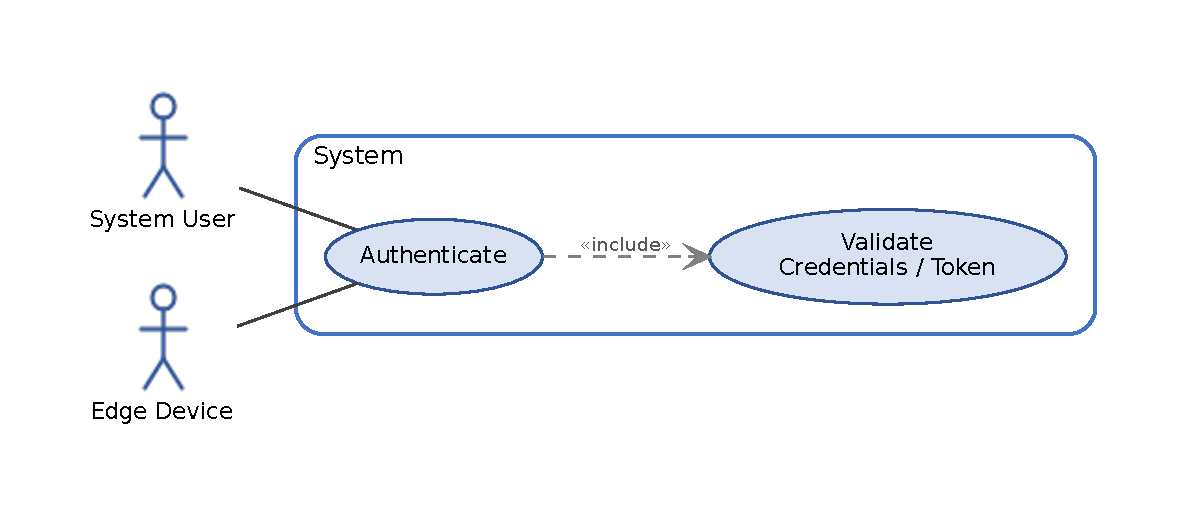
\includegraphics[width=0.8\textwidth,height=4.3cm,keepaspectratio]{figures/usecase/uc01.pdf}\par}

\noindent\textbf{UC-02 Manage User Accounts.} \textit{Actor:} System Administrator. \textit{Intent:} create, update, deactivate users and assign roles.

{\centering 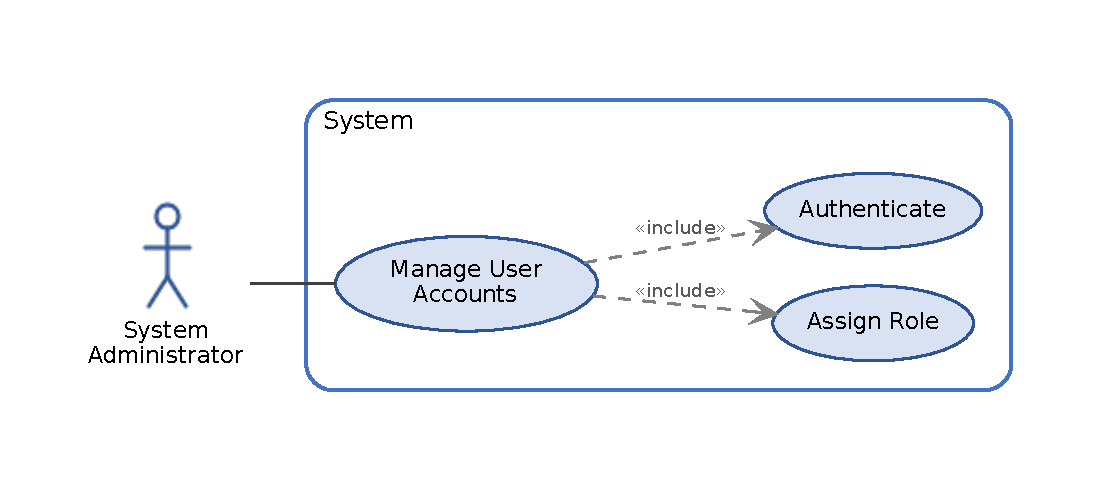
\includegraphics[width=0.8\textwidth,height=4.3cm,keepaspectratio]{figures/usecase/uc02.pdf}\par}

\noindent\textbf{UC-03 Configure System \& Thresholds.} \textit{Actor:} System Administrator. \textit{Intent:} set environmental thresholds, hysteresis, and device configuration pushed to the edge.

{\centering 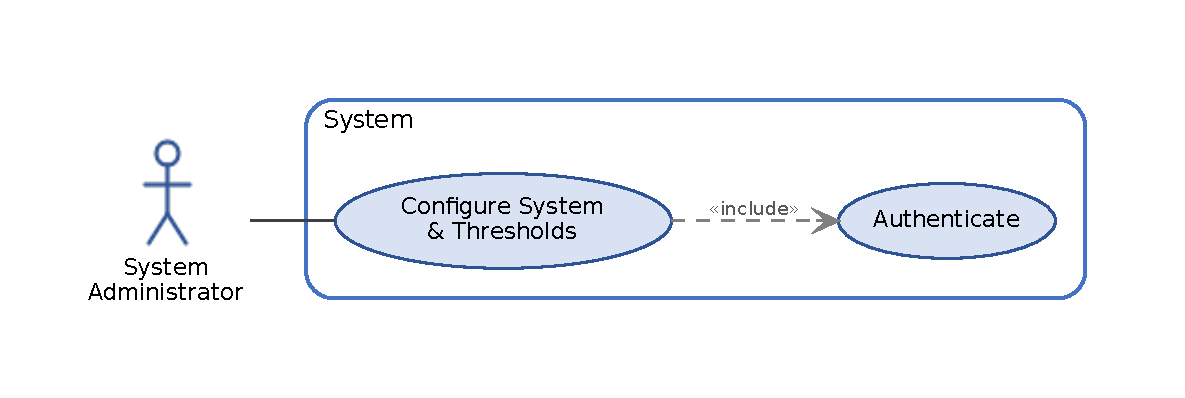
\includegraphics[width=0.8\textwidth,height=4.3cm,keepaspectratio]{figures/usecase/uc03.pdf}\par}

\noindent\textbf{UC-04 Manage Farms.} \textit{Actor:} Farm Owner. \textit{Intent:} create and maintain farm records at the top of the hierarchy.

{\centering 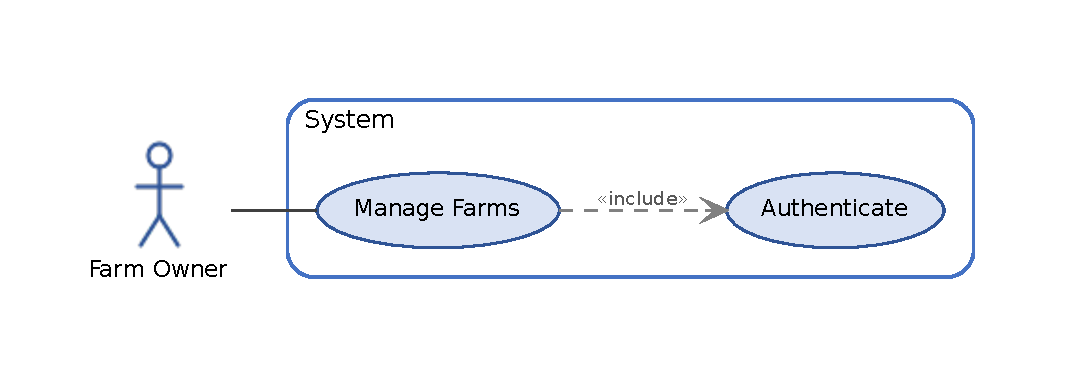
\includegraphics[width=0.8\textwidth,height=4.3cm,keepaspectratio]{figures/usecase/uc04.pdf}\par}

\noindent\textbf{UC-05 Manage Pens.} \textit{Actor:} Farm Manager. \textit{Intent:} define pens within a farm and their capacities.

{\centering 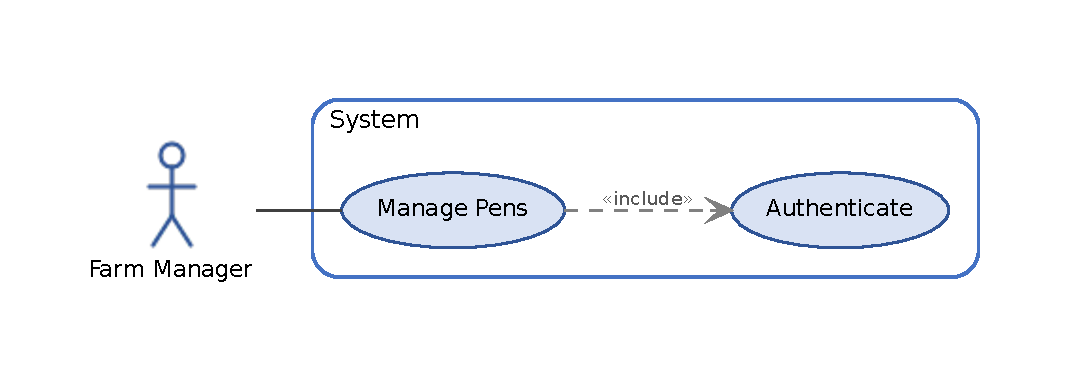
\includegraphics[width=0.8\textwidth,height=4.3cm,keepaspectratio]{figures/usecase/uc05.pdf}\par}

\noindent\textbf{UC-06 Manage Batches.} \textit{Actor:} Farm Manager. \textit{Intent:} create batches in pens and track their production cycle; validates against pen capacity.

{\centering 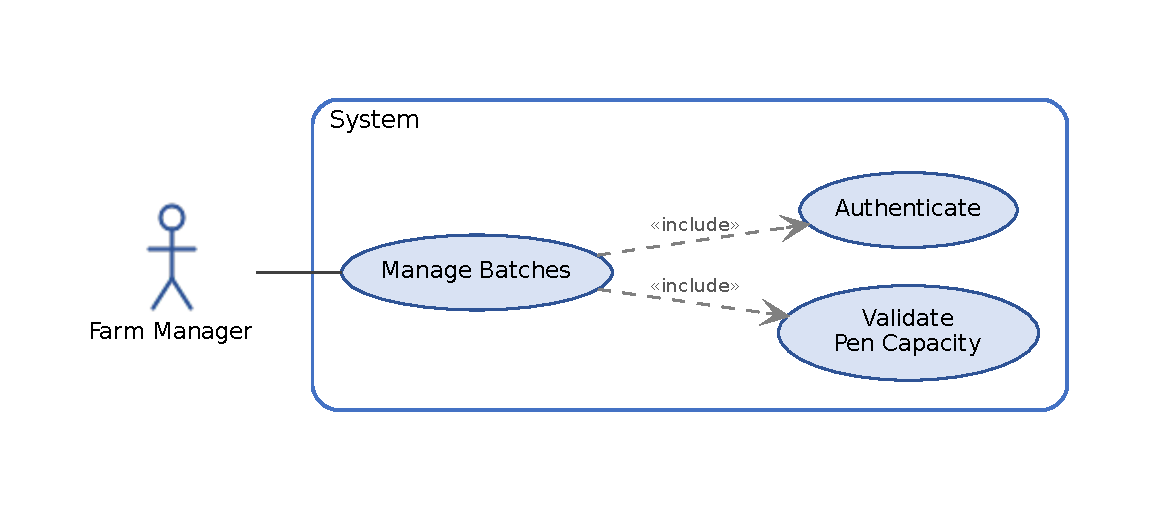
\includegraphics[width=0.8\textwidth,height=4.3cm,keepaspectratio]{figures/usecase/uc06.pdf}\par}

\noindent\textbf{UC-07 Record Chick Entry.} \textit{Actors:} Farm Worker, Farm Manager. \textit{Intent:} log arrival of chicks into a batch, setting the initial flock quantity.

{\centering 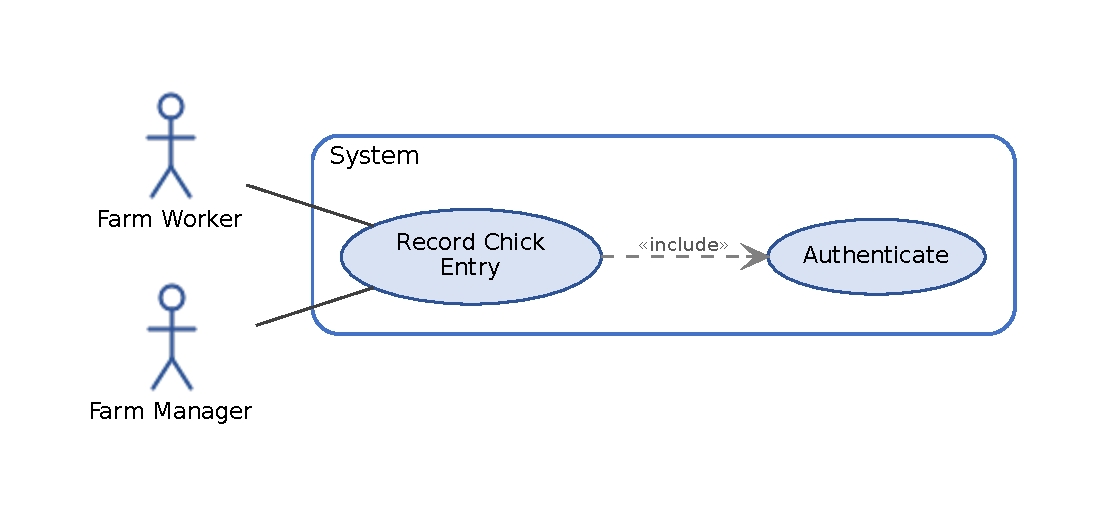
\includegraphics[width=0.8\textwidth,height=4.3cm,keepaspectratio]{figures/usecase/uc07.pdf}\par}

\noindent\textbf{UC-08 Record Mortality.} \textit{Actor:} Farm Worker. \textit{Intent:} record deaths per batch; updates flock quantity and feeds mortality-rate analytics.

{\centering 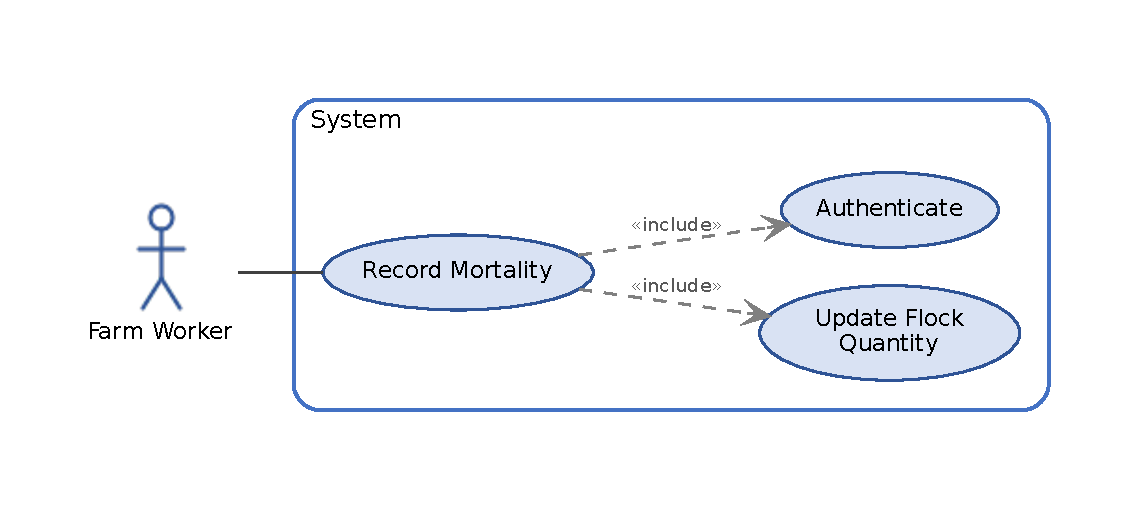
\includegraphics[width=0.8\textwidth,height=4.3cm,keepaspectratio]{figures/usecase/uc08.pdf}\par}

\noindent\textbf{UC-09 Record Feeding.} \textit{Actor:} Farm Worker. \textit{Intent:} record feed consumption; decrements feed inventory.

{\centering 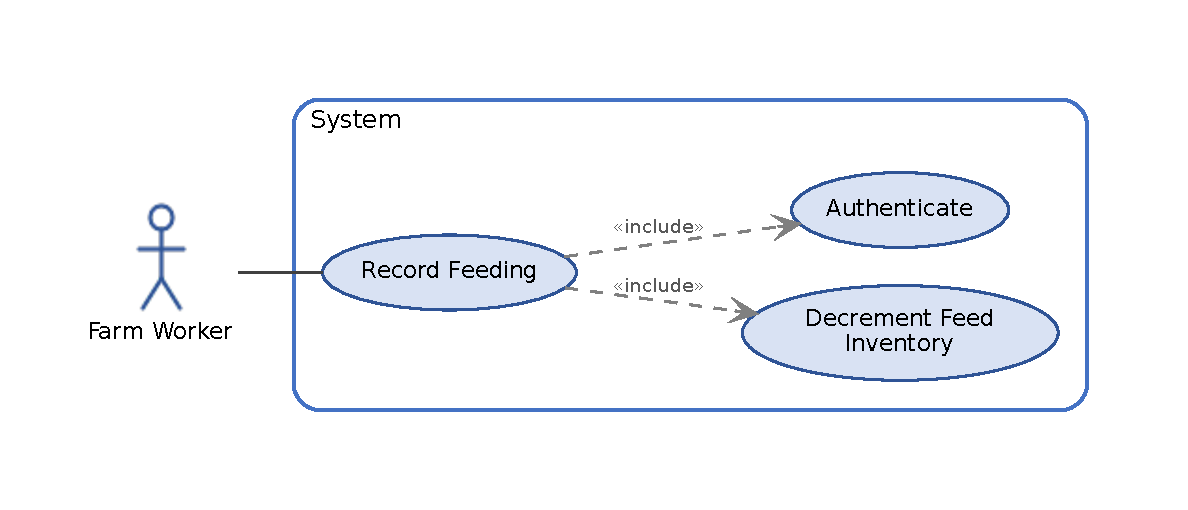
\includegraphics[width=0.8\textwidth,height=4.3cm,keepaspectratio]{figures/usecase/uc09.pdf}\par}

\noindent\textbf{UC-10 Record Health Observation.} \textit{Actors:} Farm Worker, Veterinary Consultant. \textit{Intent:} log observed health signs against a batch.

{\centering 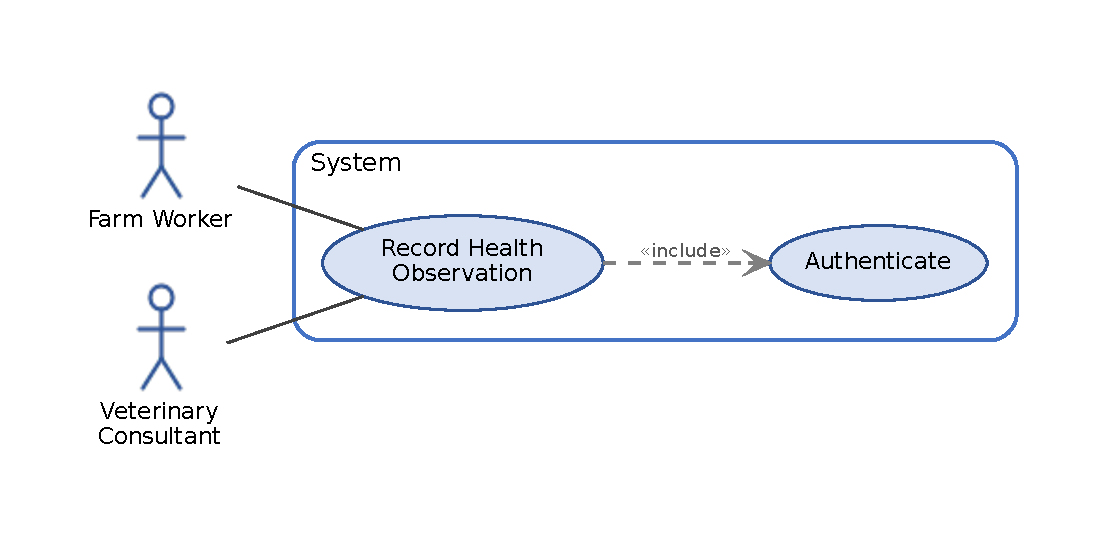
\includegraphics[width=0.8\textwidth,height=4.3cm,keepaspectratio]{figures/usecase/uc10.pdf}\par}

\noindent\textbf{UC-11 Record Treatment.} \textit{Actors:} Farm Manager, Veterinary Consultant. \textit{Intent:} record treatments administered to a batch.

{\centering 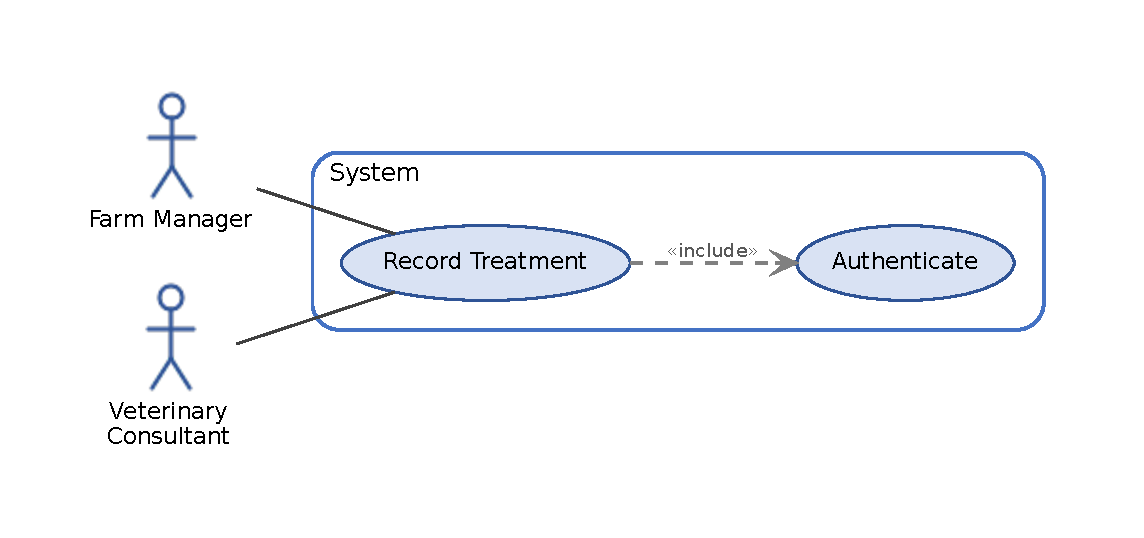
\includegraphics[width=0.8\textwidth,height=4.3cm,keepaspectratio]{figures/usecase/uc11.pdf}\par}

\noindent\textbf{UC-12 Record Vaccination.} \textit{Actors:} Farm Manager, Veterinary Consultant. \textit{Intent:} record vaccinations and schedule.

{\centering 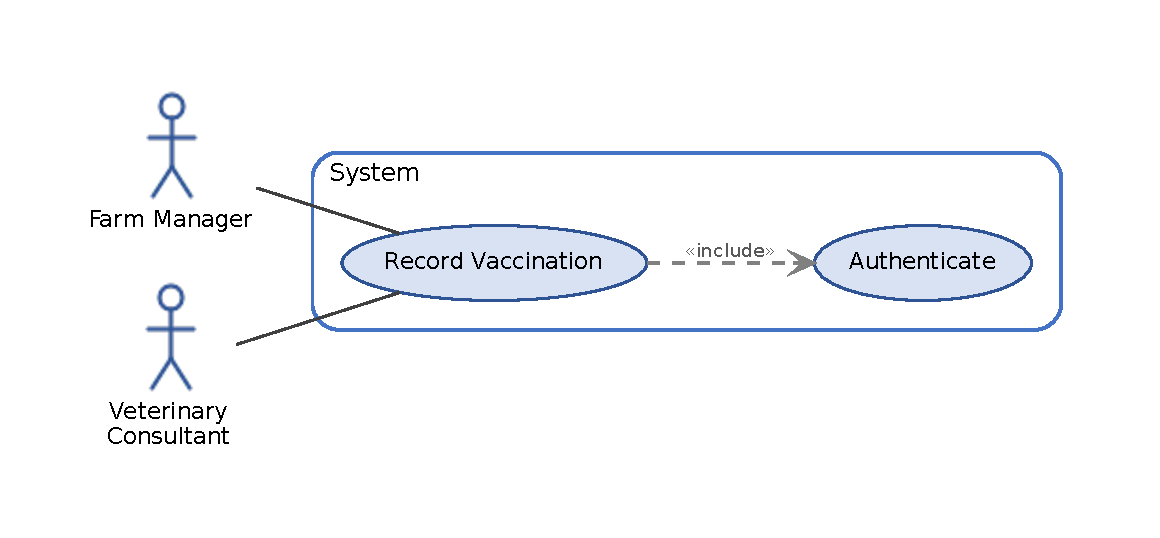
\includegraphics[width=0.8\textwidth,height=4.3cm,keepaspectratio]{figures/usecase/uc12.pdf}\par}

\noindent\textbf{UC-13 Manage Inventory.} \textit{Actor:} Farm Manager. \textit{Intent:} maintain feed and supply stock with non-negative balance rules.

{\centering 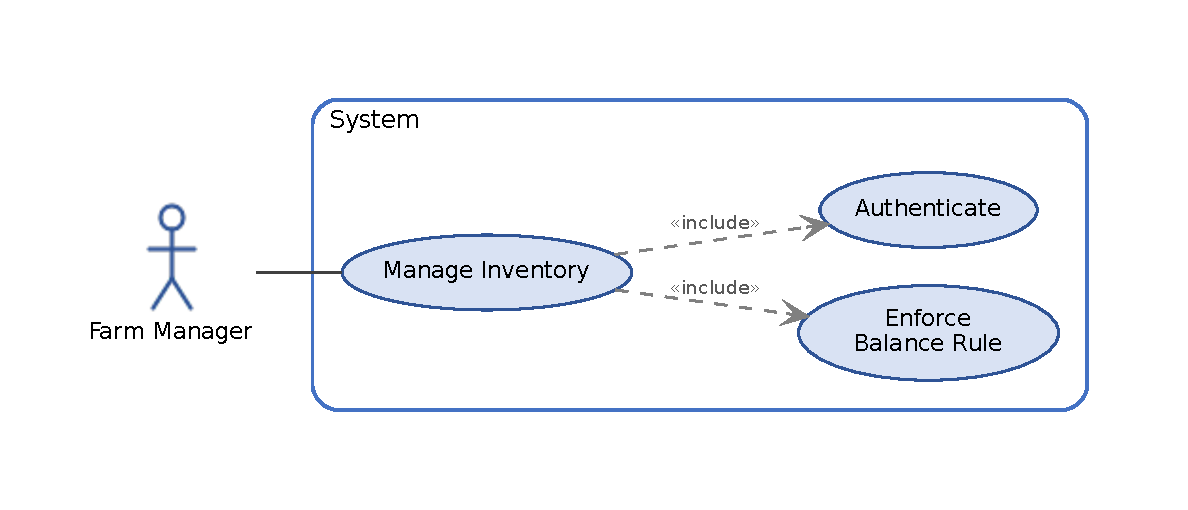
\includegraphics[width=0.8\textwidth,height=4.3cm,keepaspectratio]{figures/usecase/uc13.pdf}\par}

\noindent\textbf{UC-14 Record Expense.} \textit{Actor:} Farm Manager. \textit{Intent:} record operational expenses for cost analysis.

{\centering 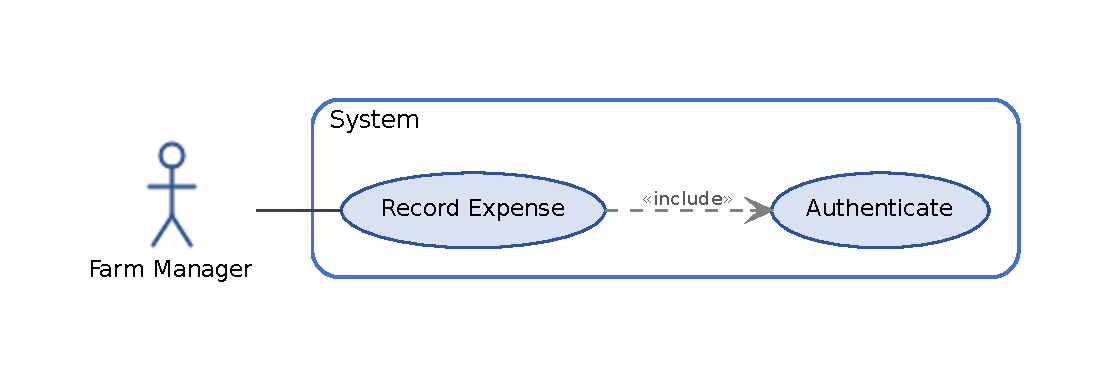
\includegraphics[width=0.8\textwidth,height=4.3cm,keepaspectratio]{figures/usecase/uc14.pdf}\par}

\noindent\textbf{UC-15 Record Sale.} \textit{Actor:} Farm Manager. \textit{Intent:} record sales linked to a batch for profitability analysis.

{\centering 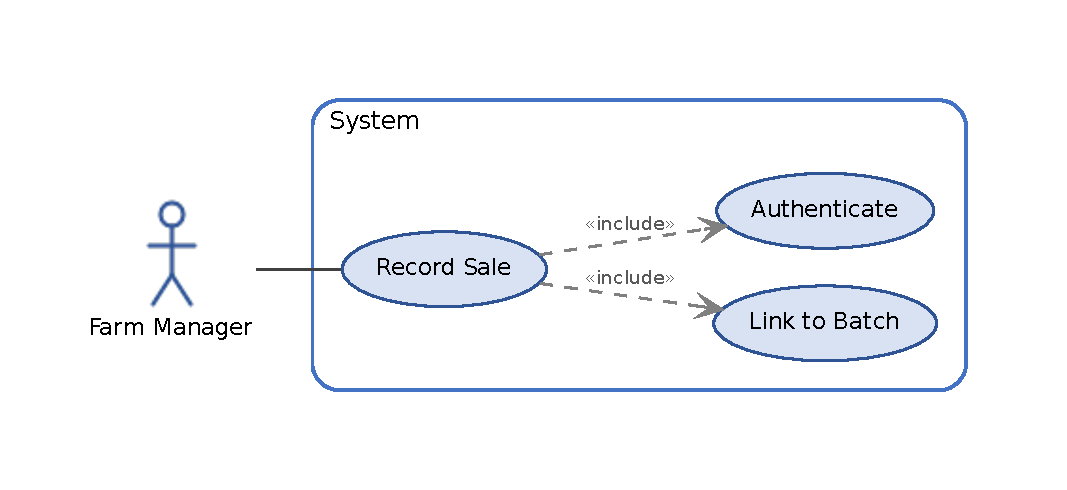
\includegraphics[width=0.8\textwidth,height=4.3cm,keepaspectratio]{figures/usecase/uc15.pdf}\par}

\noindent\textbf{UC-16 View Dashboard.} \textit{Actors:} Farm Owner, Farm Manager, Farm Worker. \textit{Intent:} view current conditions, alerts, flock status, and KPIs.

{\centering 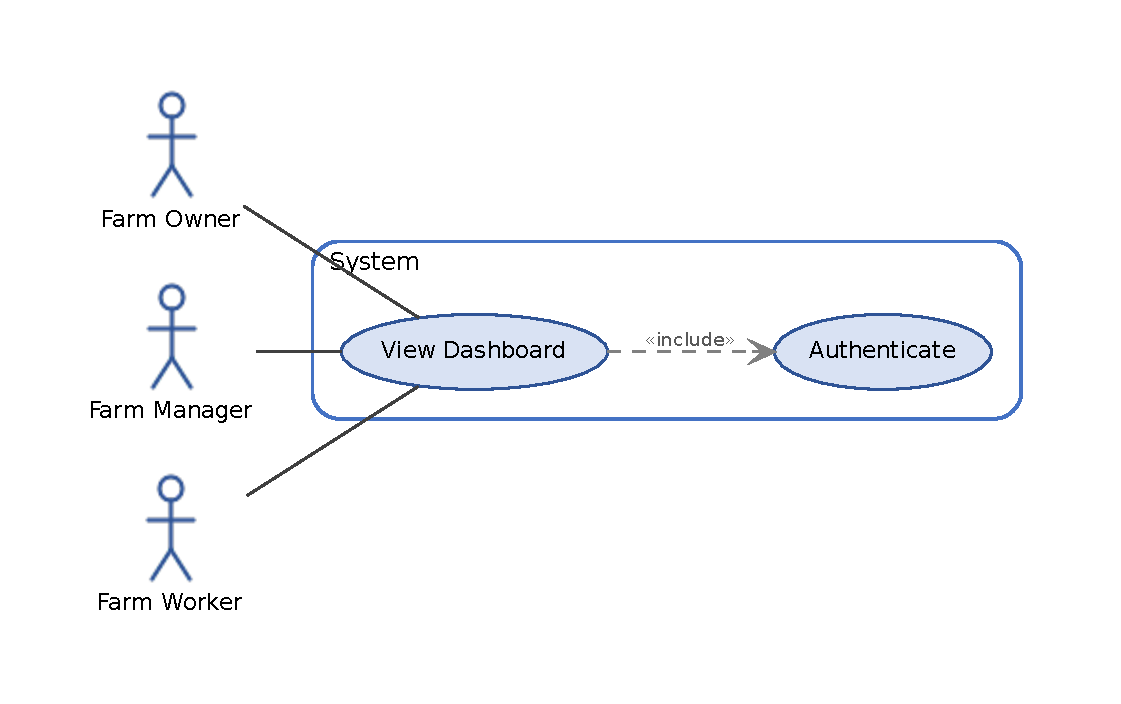
\includegraphics[width=0.8\textwidth,height=4.3cm,keepaspectratio]{figures/usecase/uc16.pdf}\par}

\noindent\textbf{UC-17 View Environmental Charts.} \textit{Actors:} Farm Manager, Veterinary Consultant. \textit{Intent:} inspect temperature, humidity, and gas-risk trends.

{\centering 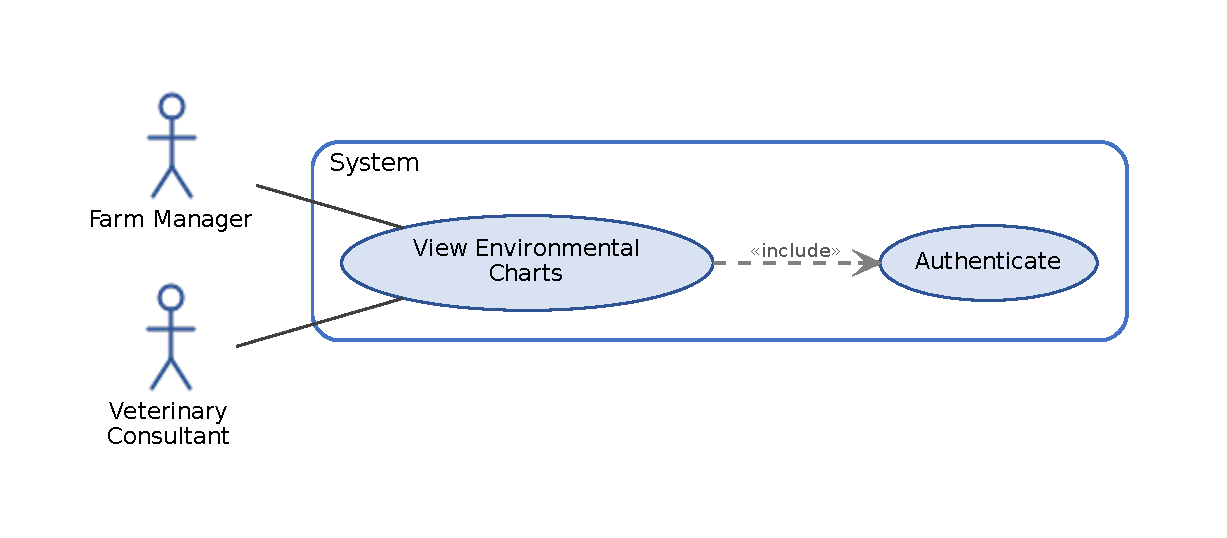
\includegraphics[width=0.8\textwidth,height=4.3cm,keepaspectratio]{figures/usecase/uc17.pdf}\par}

\noindent\textbf{UC-18 Review AI Prediction.} \textit{Actors:} Farm Manager, Veterinary Consultant. \textit{Intent:} review flagged vision results, especially \texttt{uncertain} cases, and confirm or dismiss.

{\centering 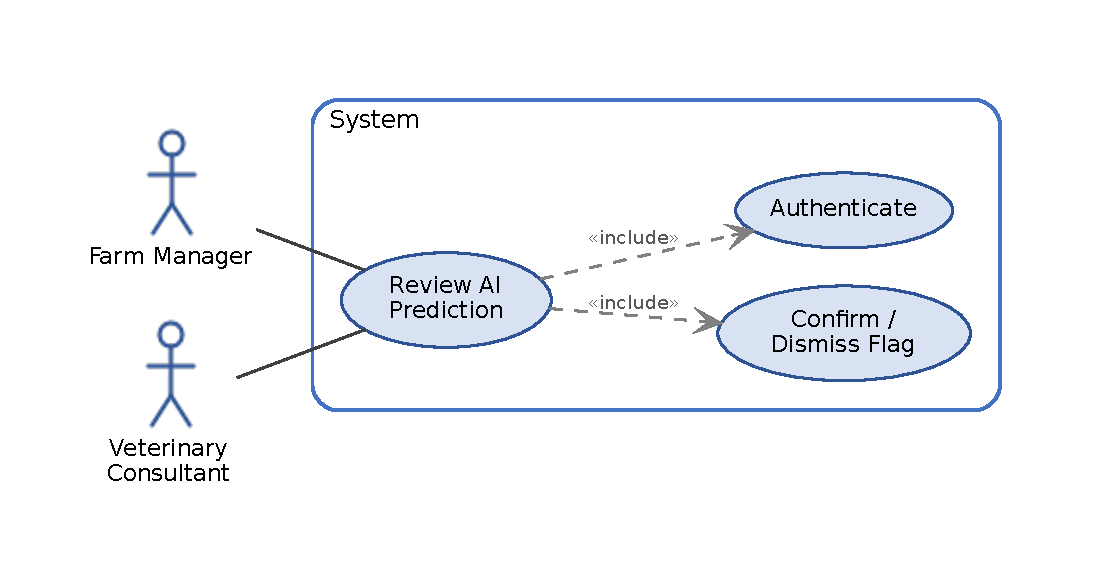
\includegraphics[width=0.8\textwidth,height=4.3cm,keepaspectratio]{figures/usecase/uc18.pdf}\par}

\noindent\textbf{UC-19 Acknowledge Alert.} \textit{Actor:} Farm Manager. \textit{Intent:} acknowledge an active warning/critical alert.

{\centering 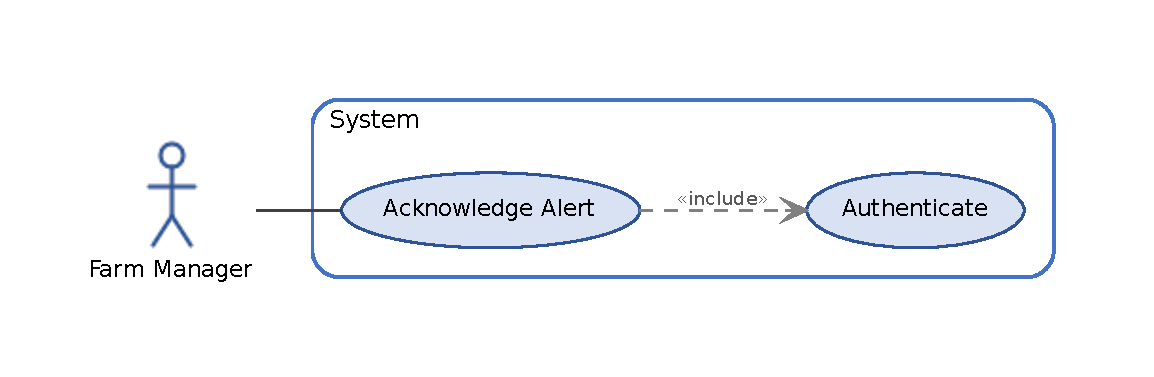
\includegraphics[width=0.8\textwidth,height=4.3cm,keepaspectratio]{figures/usecase/uc19.pdf}\par}

\noindent\textbf{UC-20 Resolve Alert.} \textit{Actor:} Farm Manager. \textit{Intent:} resolve an acknowledged alert and log the corrective action taken.

{\centering 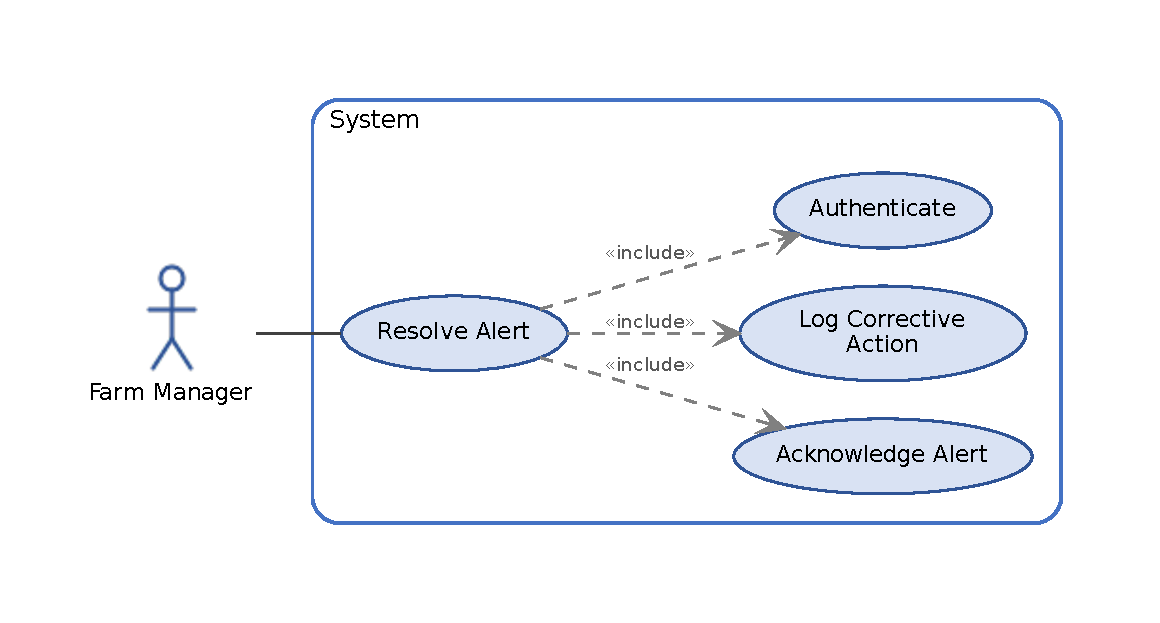
\includegraphics[width=0.8\textwidth,height=4.3cm,keepaspectratio]{figures/usecase/uc20.pdf}\par}

\noindent\textbf{UC-21 Generate Report.} \textit{Actors:} Farm Owner, Farm Manager. \textit{Intent:} produce and export production and financial reports.

{\centering 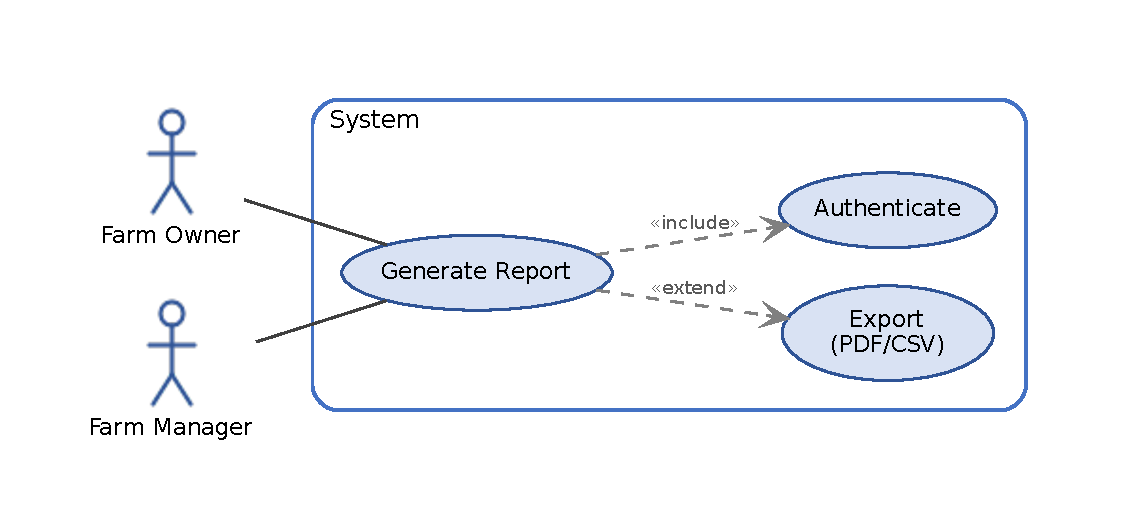
\includegraphics[width=0.8\textwidth,height=4.3cm,keepaspectratio]{figures/usecase/uc21.pdf}\par}

\noindent\textbf{UC-22 Manage Edge Devices.} \textit{Actor:} System Administrator. \textit{Intent:} register devices, issue tokens, assign a device to a pen.

{\centering 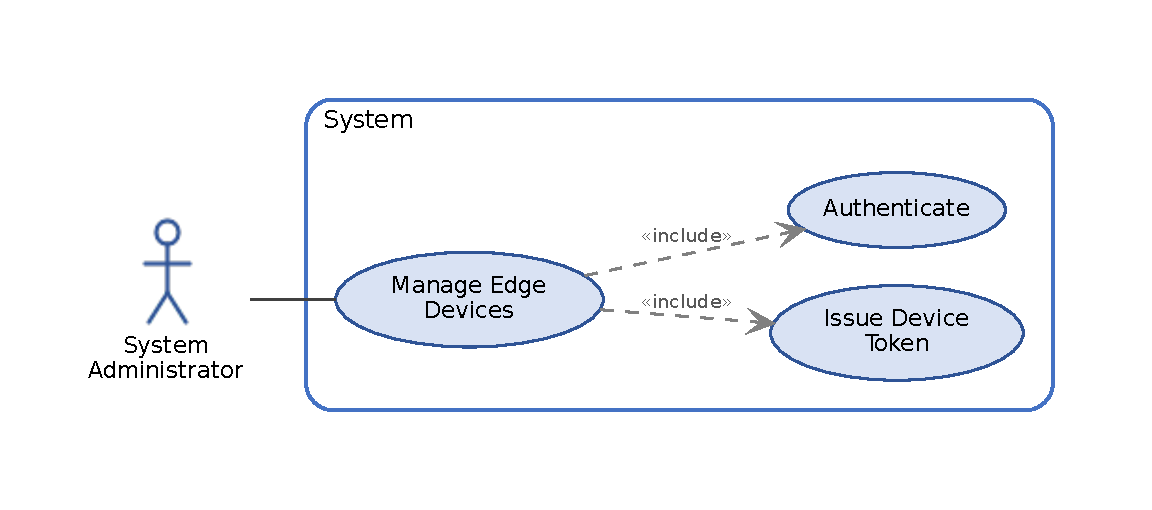
\includegraphics[width=0.8\textwidth,height=4.3cm,keepaspectratio]{figures/usecase/uc22.pdf}\par}

\noindent\textbf{UC-23 Submit Sensor Reading.} \textit{Actor:} Edge Device. \textit{Intent:} post a validated environmental reading; may extend to \emph{Raise Alert} on a threshold breach.

{\centering 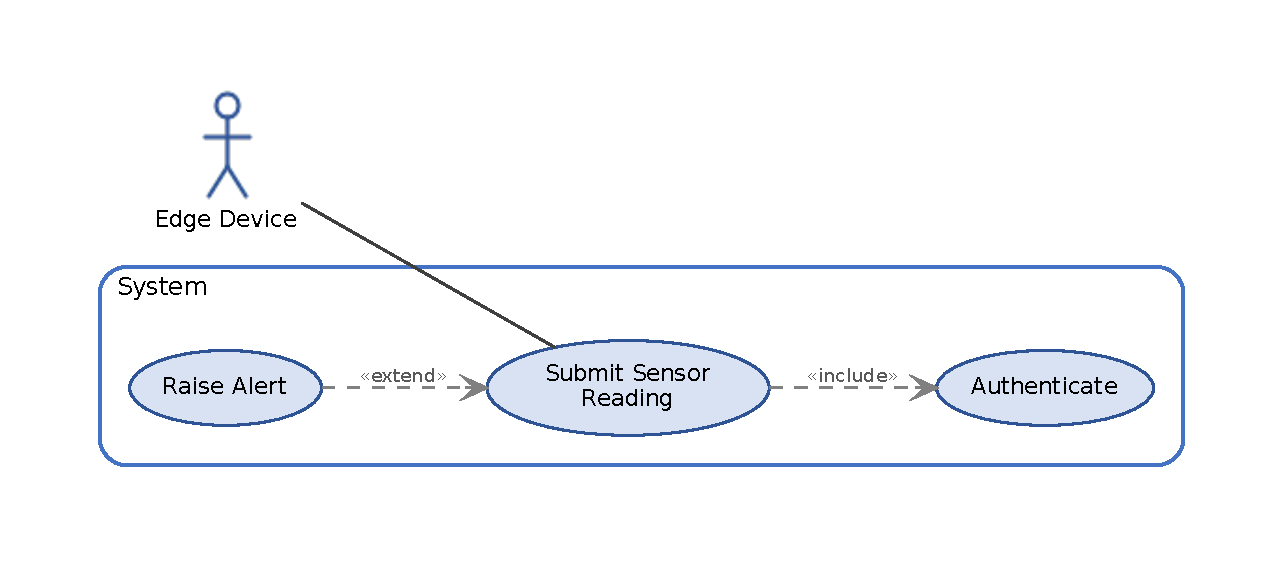
\includegraphics[width=0.8\textwidth,height=4.3cm,keepaspectratio]{figures/usecase/uc23.pdf}\par}

\noindent\textbf{UC-24 Submit Vision Result.} \textit{Actor:} Edge Device. \textit{Intent:} post a classification/detection result; may extend to \emph{Raise Alert} on a visible-risk class.

{\centering 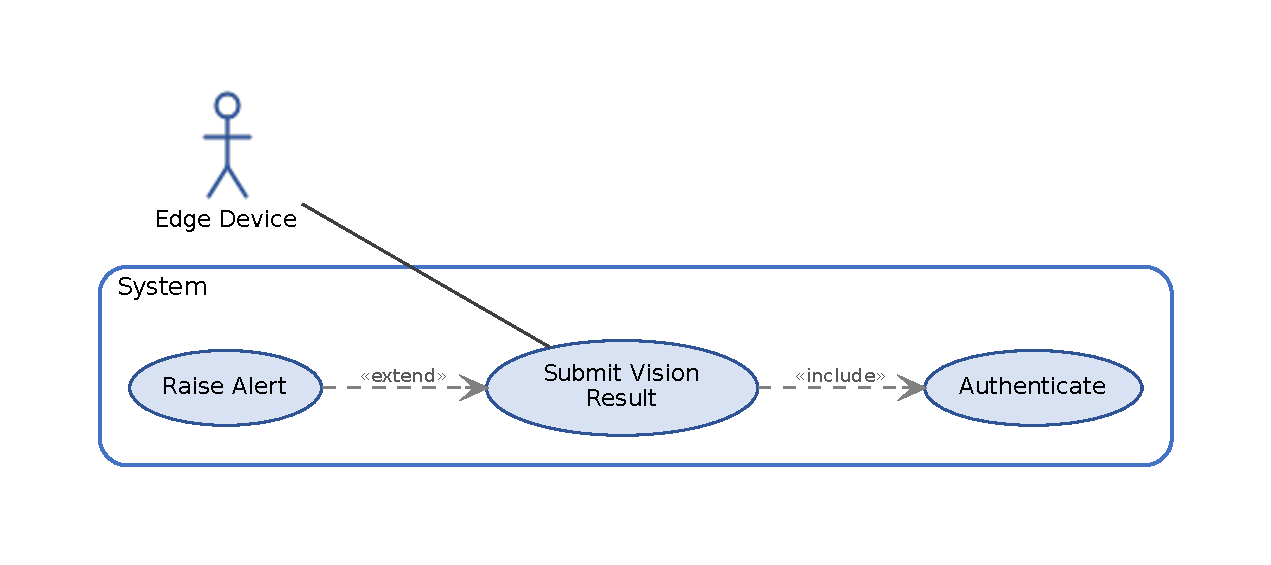
\includegraphics[width=0.8\textwidth,height=4.3cm,keepaspectratio]{figures/usecase/uc24.pdf}\par}

\noindent\textbf{UC-25 Send Heartbeat / Get Configuration.} \textit{Actor:} Edge Device. \textit{Intent:} report liveness and retrieve the current threshold configuration.

{\centering 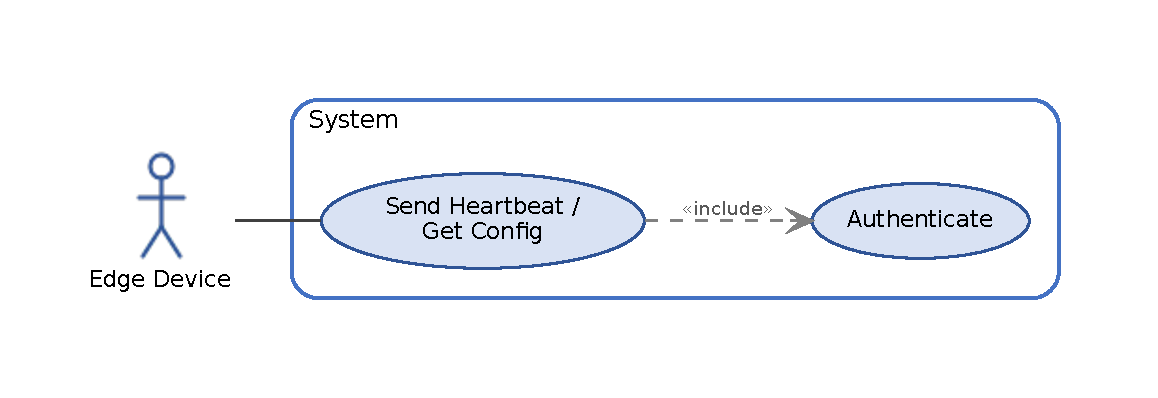
\includegraphics[width=0.8\textwidth,height=4.3cm,keepaspectratio]{figures/usecase/uc25.pdf}\par}

Together these diagrams enumerate the full behavioural scope of the system; the consolidated diagram of Figure~\ref{fig:usecase} composes them into a single view. Each diagram was generated from an equivalent PlantUML/StarUML model, so the models can be reproduced or edited in StarUML if required.

\subsection{Farm, Pen and Batch Management}

The application models the farm hierarchy explicitly: a farm contains one or more pens (houses), and each pen holds production batches over time. Create, read, update, and delete interfaces are provided for each entity, and every record carries a stable universally unique identifier, creation and update timestamps, and the identity of the user who created and last modified it, so that the provenance of any record can be traced. The batch is the central organising entity of the whole system, because every operational record, chick entries, mortality, feed usage, weight samples, health observations, sensor readings, and vision results, is keyed to a batch and thereby to a pen and its monitoring device; this single anchor is what allows the otherwise-separate data streams to be correlated. Validation enforces the domain rules, ensuring for example that a batch references a valid pen within a farm the user is permitted to access, that batch codes are unique within a farm, and that a batch's live population is never edited directly but is instead derived from its transactions, as detailed in the flock-balance logic of Section~3.10.13. A batch also carries a status lifecycle, planned, active, closed, and archived, so that historical batches remain available for reporting without cluttering the operational views. Access is scoped by role and by farm assignment, so that a worker sees only the pens and batches of the farm to which they are assigned.

\subsection{Mortality and Health Records}

Mortality records capture date, batch, count, and cause, and feed batch-level mortality-rate calculations; health records capture observations, treatments, and vaccinations, supporting the correlation of health outcomes with environmental conditions. The design intent is that these records are not merely archival but analytical: because each mortality and health entry is keyed to a batch, and each batch to a pen and thus to the device monitoring that pen, the system can align a spike in deaths with the environmental and vision records from the same period, turning the disparate streams into a single, queryable history. This is the concrete mechanism by which the integration promised in Chapter~2 is realised at the data level, and it is what distinguishes the proposed FMIS from a paper ledger, in which such correlation is impossible in practice. Validation rules guard the integrity of these records, for example rejecting a mortality count that would drive a batch's surviving quantity below zero, so that the derived mortality rate remains meaningful.

\subsection{Feed and Inventory Management}

Feeding is recorded as discrete usage events, each attributing a quantity of a given feed type to a batch on a date, so that cumulative feed consumption and, where weight samples exist, the feed-conversion ratio can be computed per batch; because feed is the dominant variable cost in broiler production, this record is central to any credible cost analysis. Inventory is modelled not as a single editable stock figure but as an append-only ledger of stock movements: the available quantity of any item is derived as its opening stock plus the sum of its signed movements, where receipts and positive adjustments add and issues, expiry, damage, and negative adjustments subtract. This ledger design preserves a full, auditable history and makes a class of silent stock-corruption errors impossible, since the balance is always reconstructable from its movements. A balance rule prevents an item from being driven negative unless an explicitly authorised adjustment is made, and a configurable reorder level flags an item as low-stock on the dashboard so that shortages are anticipated rather than discovered. To keep the feed and inventory records consistent, recording a feed-usage event automatically issues the corresponding quantity from the linked inventory item, so that physical consumption and the stock ledger cannot drift apart. Medication stock is handled analogously, with treatments optionally decrementing the linked item.

\subsection{Expenses and Sales}

The finance modules record the two sides of the farm's cash flow. Expenses are captured under a controlled set of categories, feed, medication and health, labour, utilities, equipment, chick purchase, and other, and are optionally attributed to a batch so that the cost of a production cycle can be assembled from its constituent expenses. Sales record the disposal of birds and carry a status lifecycle of draft, confirmed, and cancelled; a sale is validated so that its quantity cannot exceed the batch's available live population, and only a confirmed sale reduces that population, which is the point at which the finance module and the flock-balance logic of Section~3.10.13 meet. Each sale may accrue one or more payments, from which the amount paid and the outstanding balance are derived, supporting the tracking of credit sales that are common in smallholder trade. Because expenses and sales are both keyed to the batch, the system can compute a per-batch profitability statement, setting revenue against the chick, feed, medication, and other costs of the same batch, which is precisely the analysis a paper ledger makes impractical. In keeping with the role model, the entire finance area is restricted to owner, manager, and administrator roles and is inaccessible to farm workers, so that sensitive commercial information is confined to those authorised to see it.

\subsection{IoT and Machine-Learning Monitoring}

The monitoring modules surface the data submitted by the edge device. Each sensor reading stores the temperature, relative humidity, raw gas value, processed gas-risk value and category, sensor and actuator states, and a data-quality flag, together with the device, pen, and batch to which it belongs and both the device and server timestamps; readings that fail plausibility validation are retained but marked as rejected, so that faults are visible rather than silently discarded. These readings are presented both as a live view of current conditions and as historical charts of temperature, humidity, and gas-risk over a selectable date range, rendered with Chart.js from server-side aggregated queries so that a long history can be visualised without transferring an unbounded dataset to the browser. Device health is tracked through periodic heartbeats and a last-seen timestamp, from which each device is shown as online or offline, and actuator events are logged so that the ventilation and heating history can be reviewed. Vision results are presented through a dedicated prediction-review interface in which an authorised reviewer, a manager or the veterinary consultant, sees the model's predicted class, confidence, and detections and may accept the prediction, correct its class, mark it uncertain, flag it as a false alert, or escalate it. Crucially, the original machine output is never overwritten: corrections and review notes are stored alongside it, preserving an honest record of what the model produced and what a human decided, and an escalated case may be linked to a formal health observation for follow-up.

\subsection{Alert Management}

Alerts generated from environmental thresholds or vision results progress through a defined lifecycle, normal, warning, critical, acknowledged, resolved, shown in Figure~\ref{fig:alertstate}; the alert-handling activity, from detection through acknowledgement to resolution and logging of corrective action, is shown in Figure~\ref{fig:activity}.

\inlinefig{figures/generated/alert_state_diagram.pdf}{0.68\textwidth}{Alert lifecycle state diagram}{fig:alertstate}
\dedicatedfig{figures/generated/activity_diagram.pdf}{Activity diagram for alert detection, response and resolution}{fig:activity}

\subsection{Reporting and Analytics}

Dashboards aggregate current conditions, active alerts, flock status, mortality rate, and financial summaries into key performance indicators and Chart.js visualisations, supporting evidence-based decisions and exportable reports. Consistent with the caution against information overload noted in Chapter~2, the reporting layer is designed around a small set of decision-relevant indicators rather than an exhaustive display: the landing dashboard foregrounds the current environmental state, any active alerts, and the flock's headline status, relegating detailed histories and financial breakdowns to secondary views reached on demand. Reports are parameterised by batch and by date range so that an owner can, for instance, produce a per-batch profitability statement or a mortality-versus-conditions summary for a chosen cycle, and are exportable to PDF or CSV for record-keeping and for sharing with a veterinary consultant or a lender. The analytics deliberately privilege at-a-glance comprehension for a non-specialist operator over analytical completeness, on the reasoning that a report which is understood and acted upon is worth more than one which is comprehensive but ignored.

\subsection{UML Analysis}

The system is analysed using UML: the use-case diagram (Figure~\ref{fig:usecase}) captures functional scope by role; the class diagram (Figure~\ref{fig:class}) captures the domain model; the activity diagram (Figure~\ref{fig:activity}) captures alert handling; the sequence diagrams (Figures~\ref{fig:seqsensor} and \ref{fig:seqml}) capture the submission protocols; and the component and deployment diagrams (Figures~\ref{fig:component} and \ref{fig:deploy}) capture the software structure and physical deployment.

\inlinefig{figures/generated/class_diagram.pdf}{\textwidth}{Domain class diagram of the farm-management system}{fig:class}

\subsection{Database Design}

The database is designed in third normal form and implemented in PostgreSQL. The entity--relationship diagram (Figure~\ref{fig:erd}) defines the entities and their relationships, with referential integrity enforced through foreign keys (for example, mortality, feed, and health records reference a batch; sensor readings, vision results, and alerts reference a device) and indexing applied to timestamp and foreign-key columns for dashboard query performance. Normalising to third normal form removes the update, insertion, and deletion anomalies that would otherwise arise from redundant storage, which matters here because the same batch, pen, and device identifiers are referenced from many record types and must remain consistent as records accumulate. The choice of PostgreSQL over the lighter SQLite used in early development is deliberate: PostgreSQL provides the concurrent-write handling, transactional guarantees, and indexing maturity needed when the edge device is submitting readings at the same time as staff are entering records and dashboards are querying aggregates. Timestamp and foreign-key indexing is emphasised because the dominant query pattern, retrieving a window of readings or records for a given batch or device to render a chart, is precisely the pattern that such indexes accelerate; without them, dashboard latency would grow with the accumulating history. Client-generated UUIDs on device-submitted rows additionally allow the same physical record to be written idempotently, which is what makes the buffering-and-synchronisation behaviour of Section~3.11 safe against duplication. Table~\ref{tab:schema} summarises the core tables.

\dedicatedfig{figures/generated/erd.pdf}{Entity--relationship diagram of the system database}{fig:erd}

\begin{table}[tbp]
\caption{Core database tables}
\label{tab:schema}
\centering
\small
\begin{tabularx}{\textwidth}{|l|X|}
\hline
\rowcolor{headerblue}
\textbf{Table} & \textbf{Purpose / key fields} \\
\hline
users & Accounts and roles (username, role, email) \\
\hline
farms, pens, batches & Farm hierarchy (codes, capacity, breed, start date, initial quantity) \\
\hline
mortality, feed, health, treatments, vaccinations & Operational records linked to batches \\
\hline
inventory, expenses, sales & Stock and financial records \\
\hline
devices & Edge devices (uuid, token, pen, last\_seen) \\
\hline
sensor\_readings & Timestamped temp/humidity/gas with computed level \\
\hline
vision\_results & Timestamped class and confidence \\
\hline
alerts & Alert type, severity and status \\
\hline
audit\_records & Immutable log of significant actions \\
\hline
\end{tabularx}
\end{table}

\subsection{REST API Design}

The REST API, designed around the resources of the data model and shown in Figure~\ref{fig:restapi}, exposes endpoints for device authentication, sensor-reading submission, vision-result submission, heartbeat, configuration retrieval, and alert retrieval and acknowledgement. Submissions are authenticated with a per-device token over HTTPS, carry a client-generated UUID and a device timestamp, and are processed idempotently so that retried submissions do not create duplicates.

\inlinefig{figures/generated/rest_api_integration.pdf}{\textwidth}{REST API endpoints between the Raspberry Pi and the Django server}{fig:restapi}

\subsection{User-Interface Design}

The interface was designed around a consistent application shell, a fixed left navigation sidebar, a top bar carrying the page title and the signed-in user's role, and a content area, so that every screen shares the same structure and a non-specialist user need learn the layout only once. Before implementation, low-fidelity wireframes were produced to fix the placement of the principal interface elements independently of visual styling; the four representative wireframes in Figures~\ref{fig:wf_auth} and~\ref{fig:wf_list} correspond respectively to the authentication and dashboard screens and to the list (index) and data-entry-form screens that recur throughout the application. The authentication wireframe (Figure~\ref{fig:wf_auth}a) centres a single sign-in card on a branded background; the dashboard wireframe (Figure~\ref{fig:wf_auth}b) arranges the key indicators as a row of summary cards above environmental, alert, prediction, and inventory panels; the list wireframe (Figure~\ref{fig:wf_list}a) places a search field and an add-record control above a paginated table; and the form wireframe (Figure~\ref{fig:wf_list}b) stacks labelled input fields within a card above the save and cancel actions. Bootstrap~5 was chosen to realise these wireframes as a responsive grid that adapts to desktop and mobile browsers, with the palette fixed to a green-and-white agricultural theme in which red, amber, and blue are reserved for critical, warning, and informational states. The implemented screens that realise these wireframes are presented in Chapter~4.

\begin{figure}[tbp]\centering
 \IfFileExists{figures/generated/wireframe_login.pdf}{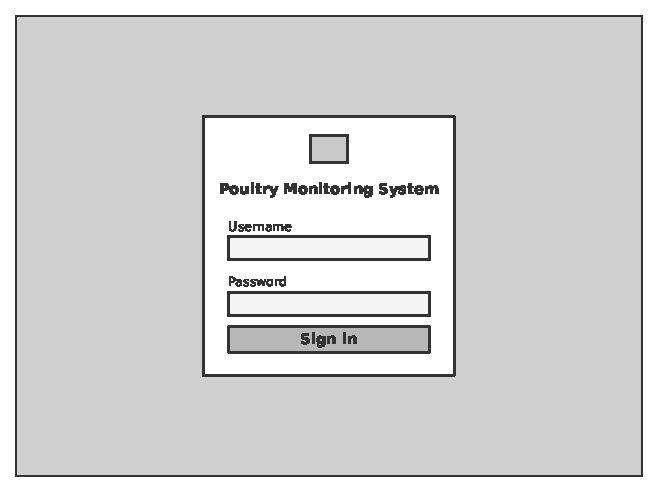
\includegraphics[width=0.78\textwidth]{figures/generated/wireframe_login.pdf}}{\fbox{\parbox[c][5cm][c]{0.78\textwidth}{\centering Wireframe: login}}}\\[3pt]
 {\footnotesize (a) Login screen}\\[10pt]
 \IfFileExists{figures/generated/wireframe_dashboard.pdf}{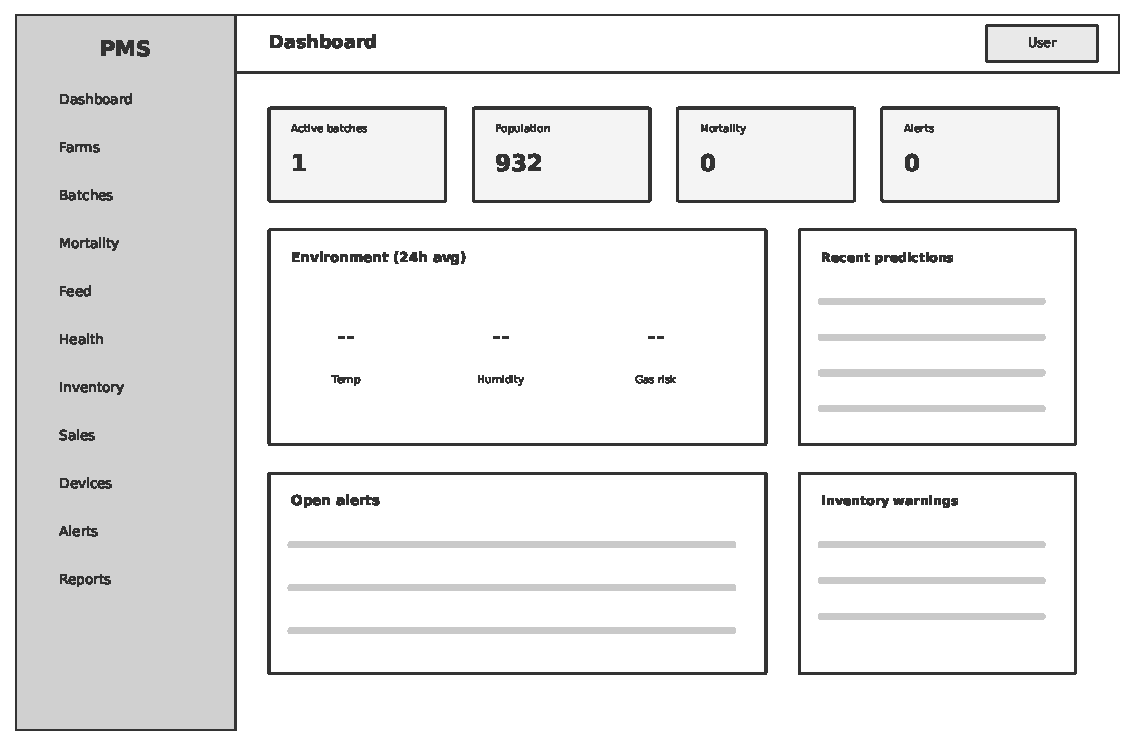
\includegraphics[width=0.92\textwidth]{figures/generated/wireframe_dashboard.pdf}}{\fbox{\parbox[c][5cm][c]{0.92\textwidth}{\centering Wireframe: dashboard}}}\\[3pt]
 {\footnotesize (b) Dashboard}
\caption{Wireframes of the authentication and dashboard screens}\label{fig:wf_auth}
\end{figure}

\begin{figure}[tbp]\centering
 \IfFileExists{figures/generated/wireframe_list.pdf}{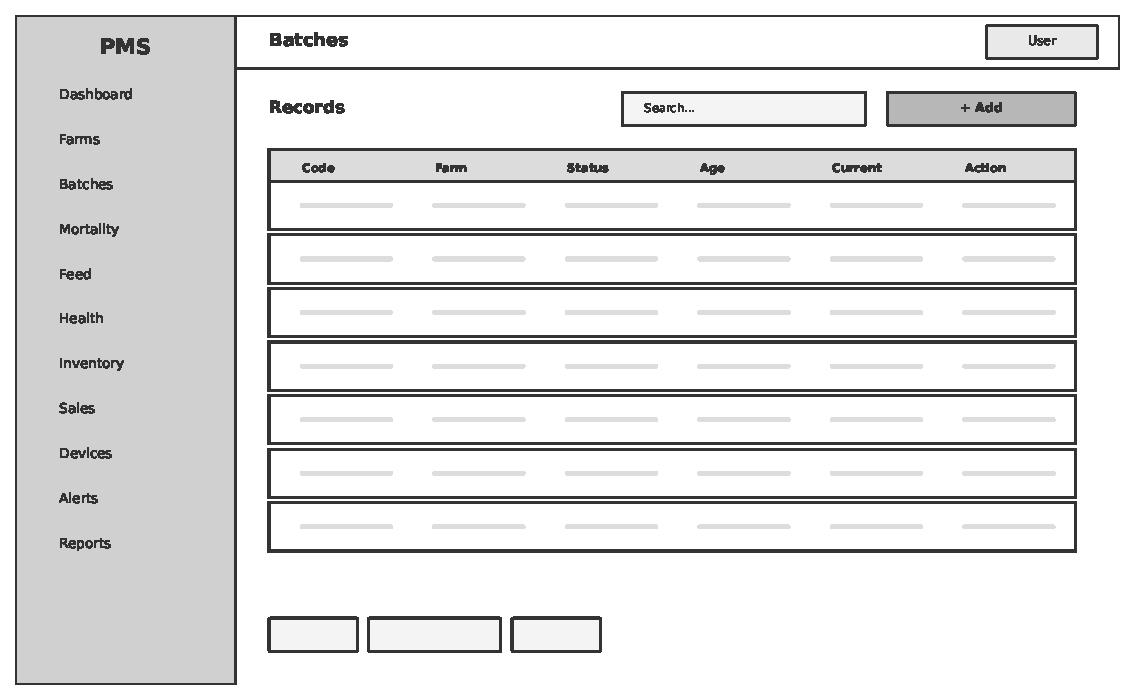
\includegraphics[width=0.92\textwidth]{figures/generated/wireframe_list.pdf}}{\fbox{\parbox[c][5cm][c]{0.92\textwidth}{\centering Wireframe: list}}}\\[3pt]
 {\footnotesize (a) List / index screen}\\[10pt]
 \IfFileExists{figures/generated/wireframe_form.pdf}{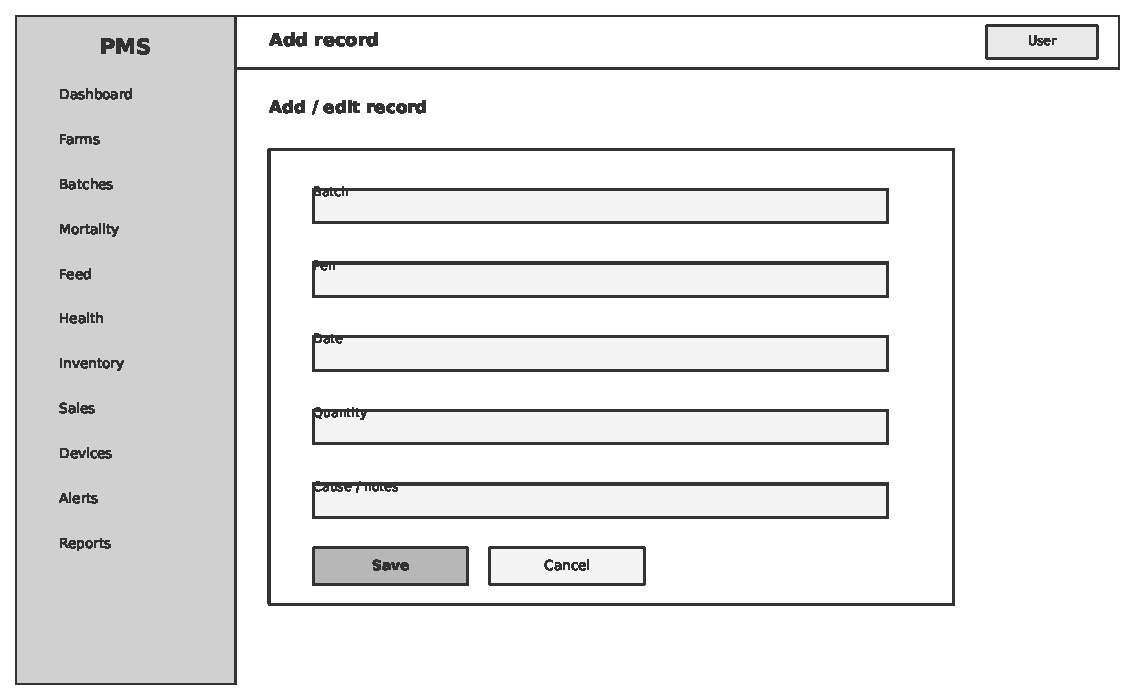
\includegraphics[width=0.92\textwidth]{figures/generated/wireframe_form.pdf}}{\fbox{\parbox[c][5cm][c]{0.92\textwidth}{\centering Wireframe: form}}}\\[3pt]
 {\footnotesize (b) Data-entry form screen}
\caption{Wireframes of a list (index) screen and a data-entry form screen}\label{fig:wf_list}
\end{figure}

\subsection{Implementation Procedure}

Implementation follows Django conventions: models define the schema and business rules; serializers and forms validate input; views and DRF viewsets implement behaviour and enforce permissions; templates render the interface; and migrations manage schema evolution. The component structure is shown in Figure~\ref{fig:component}.

\dedicatedfig{figures/generated/component_diagram.pdf}{Component diagram of the software system}{fig:component}

\subsection{Software Testing}

The application is tested at multiple levels: unit tests for models, business rules, and views; API tests (using Postman and automated test cases) for the REST endpoints, including authentication and idempotency; integration tests for end-to-end submission; security tests for authentication, authorisation, and input validation; and usability testing with farm operators. Test outcomes will be reported in Chapter~4.

\section{Integration of the Three Subsystems}

Integration unites the IoT, machine-learning, and web subsystems, as conceptualised in Figure~\ref{fig:three_subsystem} and deployed as in Figure~\ref{fig:deploy}. The complete data flow is: (1) sensors collect environmental data; (2) the camera captures frames; (3) the Raspberry Pi validates inputs; (4) environmental data are filtered; (5) images are preprocessed; (6) the model performs inference; (7) environmental and visual risk are evaluated together; (8) alerts are generated; (9) fan or heater actions are triggered where necessary; (10) data are stored locally; (11) records are transmitted through the REST API; (12) Django validates each request; (13) PostgreSQL stores the records; (14) dashboards are updated; (15) users receive alerts; (16) users acknowledge and resolve alerts; (17) corrective actions are stored; and (18) records buffered during an outage synchronise on reconnection. The submission protocols are detailed in the sequence diagrams of Figures~\ref{fig:seqsensor} and \ref{fig:seqml}. Integration relies on device authentication with per-device API tokens, HTTPS transport, client-generated UUIDs, device and server timestamps, idempotent processing with bounded retry, local buffering to prevent data loss, duplicate prevention keyed on UUIDs, a periodic device heartbeat, server-side configuration retrieval, failure-recovery on reconnection, and audit logging of submissions and acknowledgements.

\dedicatedfig{figures/generated/deployment_diagram.pdf}{Deployment diagram of the integrated system}{fig:deploy}
\inlinefig{figures/generated/sensor_submission_sequence.pdf}{\textwidth}{Sequence diagram: sensor-data submission and acknowledgement}{fig:seqsensor}
\inlinefig{figures/generated/ml_result_submission_sequence.pdf}{\textwidth}{Sequence diagram: machine-learning result submission and alerting}{fig:seqml}

\section{Overall System Architecture}

The overall architecture (Figure~\ref{fig:overall}) is layered: a perception layer (DHT22, gas sensor with ADC, camera); an edge layer (Raspberry Pi performing validation, filtering, inference, control, and buffering); a communication layer (REST over HTTPS with token authentication); an application layer (Django with DRF, PostgreSQL, dashboards, alerts, and reports); and a user layer (owner, manager, worker, and veterinary consultant). This layering localises welfare-critical functions at the edge so that they continue during network outages, while centralising records and analytics on the server.

\section{Data Collection Methods}

Two kinds of data are collected. Operational data, sensor readings, vision results, and manually entered farm records, are collected continuously by the deployed system. Evaluation data, ground-truth environmental readings from reference instruments, ground-truth health observations for validating vision outputs, system logs for reliability and latency, and operator questionnaire responses for usability, are collected during the testing phase. Locally captured images and video for model training are collected as described in Section~3.9.3.

\section{Experimental and Testing Procedures}

Testing proceeds from component to system level. Hardware is bench-tested against reference instruments and then field-tested in the poultry house. The model is evaluated on a held-out test set and then in situ. The web application is unit-, API-, integration-, security-, and usability-tested. The integrated system is tested end-to-end, including deliberate network interruption to verify buffering and synchronisation, and deliberate threshold breaches to verify alerting and actuation. All procedures are specified here; their results are reserved for Chapter~4.

\section{Evaluation Metrics}

The system is evaluated with metrics appropriate to each subsystem. For the classification stage, accuracy, precision, recall, specificity, and the F1-score are used; for the object detector, Intersection over Union (IoU) and mean Average Precision (mAP@0.5 and mAP@0.5:0.95) are used. Operational metrics include the false-positive (false-alert) rate, the false-negative (missed-distress) rate, inference latency, frames per second, model size, and memory consumption. Let $TP$, $TN$, $FP$, and $FN$ denote true positives, true negatives, false positives, and false negatives. The classification metrics are defined as:

\begin{equation}
\text{Accuracy} = \frac{TP + TN}{TP + TN + FP + FN}
\end{equation}
\begin{equation}
\text{Precision} = \frac{TP}{TP + FP}, \qquad
\text{Recall (Sensitivity)} = \frac{TP}{TP + FN}
\end{equation}
\begin{equation}
\text{Specificity} = \frac{TN}{TN + FP}, \qquad
\text{F1} = 2 \cdot \frac{\text{Precision} \cdot \text{Recall}}{\text{Precision} + \text{Recall}}
\end{equation}
\begin{equation}
\text{FPR} = \frac{FP}{FP + TN}, \qquad
\text{FNR} = \frac{FN}{FN + TP}
\end{equation}

For detection, the Intersection over Union between a predicted box $B_p$ and a ground-truth box $B_{gt}$ is:

\begin{equation}
\text{IoU} = \frac{\lvert B_p \cap B_{gt} \rvert}{\lvert B_p \cup B_{gt} \rvert}
\end{equation}

Average Precision (AP) is the area under the precision--recall curve for a class, and the mean Average Precision averages AP over all classes:

\begin{equation}
\text{AP} = \int_{0}^{1} p(r)\, dr, \qquad
\text{mAP} = \frac{1}{N}\sum_{i=1}^{N}\text{AP}_i
\end{equation}

where $p(r)$ is precision as a function of recall and $N$ is the number of classes; mAP@0.5 uses an IoU threshold of 0.5, while mAP@0.5:0.95 averages over IoU thresholds from 0.5 to 0.95. Inference latency is the time to process one frame, and frames per second is its reciprocal:

\begin{equation}
\text{FPS} = \frac{1}{\text{latency per frame (s)}}
\end{equation}

In the operational context, the false-alert rate (the false-positive rate applied to alerts) and the missed-distress rate (the false-negative rate applied to welfare-critical classes) are emphasised, because the cost of missing distress differs materially from the cost of a false alarm. Accuracy is reported with caution for the detection task and for imbalanced classes, where precision, recall, F1, and mAP are more informative. Non-AI metrics include end-to-end alert latency (sensor reading to dashboard notification), system uptime (reliability), and questionnaire-based usability scores; their target values are stated as acceptance criteria and assessed in Chapter~4.

\section{Reliability and Fault Handling}

Reliability is engineered through edge autonomy and graceful degradation: sensing, threshold evaluation, actuation, and logging continue on the Raspberry Pi during server or network outages, with records buffered locally and synchronised on reconnection. Sensor faults are handled by range and plausibility checks, filtering, and fail-safe defaults; transmission faults are handled by bounded retry with idempotent, UUID-keyed submission to prevent duplication; and a periodic heartbeat allows the server to detect an offline device. Actuator protection (minimum on/off times, hysteresis) reduces wear-related failure.

\section{Security Considerations}

Security measures include per-device API tokens for device authentication, user authentication with role-based authorisation, HTTPS transport for all communication, server-side input validation to prevent injection and malformed data, idempotency keys to prevent replay-induced duplication, and audit logging of significant actions. Secrets are kept out of source control, and least-privilege principles govern role permissions. Security testing validates authentication, authorisation, and validation controls.

\section{Electrical and Operational Safety}

Because the system switches mains-powered actuators near live animals, safety is treated as a first-class concern. Opto-isolated relays separate mains wiring from low-voltage logic; a fuse and circuit breaker protect against overcurrent; all mains wiring is enclosed; the heat lamp is guarded to reduce fire risk; and fail-safe control defaults avoid hazardous actuator states on sensor or power faults. The enclosure protects electronics from dust and moisture in the poultry-house environment. These measures protect the equipment, the operators, and the birds.

\section{Ethical Considerations}

The study involves animals only observationally, through environmental monitoring and non-invasive imaging, and does not subject birds to experimental procedures; the system is designed to improve welfare. Human participation is limited to farm operators providing usability feedback, from whom informed consent is obtained and whose responses are anonymised. Data from GreenFarms Poultry are treated as confidential and used solely for research. The study adheres to the ethical guidelines of the University of Bamenda, and the computer-vision component is presented explicitly as an early-warning aid requiring human or veterinary confirmation, not as an autonomous diagnostic authority. Two further ethical considerations follow from the system's design and are addressed by it. First, because the vision component makes inferences that could, if over-trusted, lead to inappropriate action on live animals, the explicit \texttt{uncertain} class and the human-in-the-loop review workflow are not merely technical features but ethical safeguards, ensuring that a low-confidence machine judgement never triggers an irreversible decision without human oversight. Second, because the system controls mains-powered actuators in an occupied animal house, the fail-safe control defaults described in Section~3.8 carry an ethical as well as an engineering weight, since their purpose is to prevent a sensor or power fault from harming the very birds the system is meant to protect. Data minimisation is also observed: imagery is captured and retained only as needed for model development and review, and no personally identifying information about staff is stored beyond what the role-based accounts require.

\section{Methodological Assumptions}

The methodology assumes that visible distress and health-risk indicators are detectable from standard RGB webcam imagery under farm lighting; that low-cost sensors, once validated against reference instruments, provide adequate signals for threshold-based decisions; that the metal-oxide gas sensor's relative output is a useful ammonia-risk proxy despite its non-selectivity; that intermittent connectivity can be tolerated through local buffering; and that public datasets, supplemented with local imagery, are sufficient to train a usable model. These assumptions are tested during evaluation.

\section{Methodological Limitations}

The methodology has acknowledged limitations: single-site evaluation at GreenFarms Poultry limits statistical generalisability; the gas sensor cannot provide selective, calibrated ammonia measurement; computer vision detects only outwardly visible conditions and is sensitive to lighting, occlusion, and density; on/off actuation lacks proportional control; and the prototype scale (one house) means that multi-house scaling is addressed only architecturally. These limitations are stated so that the validity and scope of the eventual results can be judged fairly, and they motivate the future work identified in the concluding chapter.

This chapter specified the materials and methods for the integrated system: the design-and-build research design and case-study context; the elicited requirements; the hardware, machine-learning, and software materials; the iterative development model; and the detailed methodology for each subsystem and for their integration, together with the data-collection, testing, and evaluation procedures, the evaluation formulae, and the reliability, security, safety, ethical, assumption, and limitation considerations. Throughout, the chapter described designs and procedures rather than results, and inserted compile-safe placeholders for the implementation evidence to be produced during development. The following chapter will report the results of applying these methods.

%% ══════════════════════════════════════════
%% CHAPTER 4: RESULTS AND DISCUSSION
%% ══════════════════════════════════════════
\chapter{Chapter 4: Results and Discussion}
\setcounter{section}{0}
\renewcommand{\thesection}{4.\arabic{section}}
\renewcommand{\thesubsection}{4.\arabic{section}.\arabic{subsection}}

This chapter reports the results obtained from applying the methods specified in Chapter~3 and then discusses their meaning, significance, and limitations. Following the presentation convention adopted for this dissertation, Section~4.1 states the results as factual observations, what was built, what was measured, and what was verified, without interpretation, while Section~4.2 interprets those results in relation to the specific objectives, the requirements of Section~3.4, and the literature surveyed in Chapter~2. The results are organised to follow the four specific objectives of Section~1.5 so that each objective is answered in turn and its evidence can be located without ambiguity. In keeping with good scientific practice, results that were \emph{not} obtained within the prototype's time and resource envelope, most importantly the calibration of the gas sensor against a reference ammonia concentration, the inference-latency benchmark on Raspberry Pi hardware, and any accuracy figure for the six visible-condition classes of the original design, are reported honestly as pending rather than asserted, and the reasons for their deferral are stated so that the validity and scope of the present findings can be judged fairly.

\section{Results}

\subsection{Overview of the Delivered System}

The methods of Chapter~3 yielded a working, integrated software system organised into three clearly separated subsystems, an edge client for the Raspberry Pi, a machine-learning pipeline, and a Django web application with a versioned REST interface, together with the deployment, testing, and documentation artefacts specified in the methodology. The web application was implemented as thirteen Django applications spanning accounts, farms, flocks, feeding, health, inventory, finance, IoT devices, vision, alerts, reports, auditing, and a dashboard. The relational schema was expressed as twelve database migrations that applied cleanly, and the framework's own configuration check reported no issues. The server-rendered interface comprised seventy-four HTML templates realising the green-and-white agricultural theme described in Section~3.10. Nine device-facing REST endpoints were exposed under a versioned \texttt{/api/v1/} namespace. A single management command populated the system with clearly labelled demonstration data for five role-specific user accounts, one demonstration farm, three pens, an active batch, and the associated operational, environmental, and vision records, enabling every page to be exercised with representative content.

The correctness of the delivered system was evaluated by an automated test suite executed with the \texttt{pytest} framework, following the experimental and testing procedures of Section~3.14. Across the three subsystems, seventy-four automated tests were executed and all seventy-four passed, distributed as fifty-seven backend tests, nine machine-learning tests, and eight edge-client tests. Table~\ref{tab:testsummary} summarises the outcome by subsystem and category. These figures are the measured output of the test runner and are reported without adjustment.

\begin{table}[tbp]
\centering
\caption{Automated test outcomes by subsystem}
\label{tab:testsummary}
\begin{tabularx}{\textwidth}{@{}lXcc@{}}
\toprule
\textbf{Subsystem} & \textbf{Principal areas covered} & \textbf{Tests} & \textbf{Passed} \\
\midrule
Backend (Django/DRF) & Flock balance, inventory ledger, sale/mortality validation, alert state transitions, role permissions, farm data isolation, device API, vision review, CSV export, health check & 57 & 57 \\
Machine learning & Class-mapping resolution, label and statistics tools, inference-payload contract, empty-prediction handling & 9 & 9 \\
Edge client & Durable local queue and restart recovery, idempotent enqueue, threshold-based fan/heater control, mock inference payload, heartbeat & 8 & 8 \\
\midrule
\textbf{Total} & & \textbf{74} & \textbf{74} \\
\bottomrule
\end{tabularx}
\end{table}

\subsection{Objective One: The Raspberry Pi IoT Edge Unit}

The first specific objective concerned the Raspberry Pi edge unit that measures temperature, humidity, and gas/ammonia risk and controls ventilation and heating actuators. At the software and firmware level this objective was realised as a modular edge client whose components, configuration, sensor service, camera service, on-device inference service, threshold-based control service, durable local queue, API client, heartbeat, and a local alert service, were each implemented behind hardware-adapter interfaces so that the physical drivers can be substituted without altering the control logic. The client was verified to run end-to-end in a hardware-independent mock mode: over a controlled multi-cycle run it read simulated environmental values, evaluated them, buffered the resulting records, and attempted transmission, logging one sensor record and one vision record per cycle.

Three behaviours central to the objective were confirmed by automated test. First, the threshold-based control logic raised a fan-activation event when the simulated temperature exceeded the configured maximum and a heater-activation event when it fell below the configured minimum, and, importantly, produced no further event while the state remained unchanged, demonstrating edge-triggered rather than continuous actuation. Second, the durable local queue retained unsent records in an on-disk store, reported the correct pending count, and, when re-opened after a simulated restart, still contained the buffered record, demonstrating recovery across process restarts. Third, an enqueue attempt using an identifier already present was ignored rather than duplicated, confirming client-side idempotency. Input validation at the ingestion boundary was also confirmed: a physically impossible temperature was accepted for the record but flagged with a quality of \emph{rejected} and a recorded rejection reason, so that invalid input is retained for debugging without contaminating the analysis stream.

Two stages of the iterative hardware development described in Section~3.8 are evidenced photographically. Figure~\ref{fig:breadboard} shows the assembled prototype on the bench, comprising the Raspberry Pi, breadboards, jumper wiring, a two-channel relay module, the gas sensor, a USB webcam, and a fan, with a laptop alongside displaying the \texttt{Environmental\_Monitor} source and a console line reading a temperature of 23.5\textdegree C, a humidity of 65\%, and a gas status of \emph{Normal}. Figure~\ref{fig:installed} shows the same unit on a bench inside an operating broiler house at GreenFarms Poultry, with birds visible around it and the camera on a gooseneck mount. The console line is reported here as a single observation of the monitoring loop producing output of a plausible magnitude, and as nothing more: it is one reading rather than a measurement series, and it was not taken against a reference instrument.

The DHT22 was calibrated against reference instruments across the range the deployment requires, discharging the bench-testing step of the first hardware iteration. Figure~\ref{fig:calib} plots sensor against reference for both measurands. For temperature, over a range of approximately 16 to 39\textdegree C, the fitted relationship is $Y = 0.985x + 0.2$ with a coefficient of determination of 0.998; for relative humidity, over a range of approximately 23 to 78\%, it is $Y = 0.99x + 0.1$ with a coefficient of determination of 0.999. Both slopes lie within one and a half per cent of unity and both intercepts are small relative to the width of the welfare bands defined in Section~3.8.7, so the residual systematic offset is correctable in software and no change of sensor is indicated.

What remains outstanding for this objective is the gas sensor. Its output has not been compared against a reference ammonia concentration, so no absolute calibration exists for it and it is reported throughout as a relative risk index, consistent with the position taken in Section~3.8.5. The control and buffering results reported above are unaffected either way, since they were obtained from simulated inputs against the code paths that the physical sensors are designed to feed.

\subsection{Objective Two: The Computer-Vision Model}

The second specific objective concerned a computer-vision model that detects birds and classifies visible distress or sickness risk. The machine-learning pipeline required to train, evaluate, export, and serve such a model was implemented in full and organised, as revealed by static analysis of the subsystem, into nine coherent modules covering dataset import with provenance recording, image and label verification, duplicate detection, leakage-safe splitting, dataset-configuration generation, statistics, training, evaluation, and deployment (export, inference, and benchmarking). The default detector was fixed as the lightweight YOLO11n architecture for reproducibility and edge deployment, and an optional EfficientNet classification baseline was provided for comparison. Five Jupyter notebooks covering exploratory data analysis, training, the EfficientNet baseline, evaluation, and export-and-benchmarking were produced; each is executable but ships with cleared outputs and clearly marked pending-output cells so that no result is implied before it is computed.

A configurable class-to-risk mapping was implemented as the pivotal contract linking the model to the application. Static analysis of the subsystem identified the mapping-resolution function as the most connected element of the entire machine-learning codebase, confirming its role as the central abstraction through which the six mapped classes, \texttt{healthy}, \texttt{lethargic}, \texttt{open\_beak\_stress}, \texttt{diseased\_eye}, \texttt{slipped\_tendon}, and \texttt{pendulous\_crop}, are translated into web-application risk categories and alert severities. Automated tests confirmed that a known class resolved to its documented risk category and severity (for example, \texttt{slipped\_tendon} to a \emph{mobility abnormality} of \emph{critical} severity), that an unknown class resolved safely to an \emph{uncertain} outcome rather than an error, and that the inference payload assembled from a set of detections correctly selected the highest-confidence class, attached the mapped risk category, and always fell within the valid confidence range, including the boundary case of an empty detection set.

Both stages of the vision pipeline were trained and evaluated, on the substitute datasets whose selection and licensing are recorded in Section~3.9.2. The detector is a YOLO11n model fine-tuned for forty epochs on the Broiler-Net material, whose exploratory analysis (Figures~\ref{fig:classdist} and \ref{fig:bboxdist}) recorded 3{,}211 annotated birds across twenty frames from nine video segments, tiled into 3{,}829 training and 974 validation instances of the single class \texttt{chicken}. The loss curves of Figure~\ref{fig:losscurve} show the box, classification, and distribution-focal losses falling together on both the training and the validation split across the forty epochs, without the divergence between the two that would indicate overfitting. Evaluated on the held-out validation segments, that is, on video segments not used in training, the detector attained a precision of 0.841, a recall of 0.774, an $F_1$ score of 0.806, a mean average precision at an intersection-over-union threshold of 0.5 of 0.861, and a mean average precision averaged over thresholds from 0.5 to 0.95 of 0.395; the corresponding precision--recall curve is Figure~\ref{fig:prcurve}. Exported to the ONNX interchange format, the detector ran at approximately 47 milliseconds per frame on the central processing unit of the machine used for training, which is a desktop figure and not a Raspberry Pi measurement.

The classification stage was trained on the two-class Roboflow collection, which after regrouping by source image yielded 491 bird crops, 359 for training, 66 for validation, and 66 held out for testing. On those 66 held-out crops the classifier placed all 29 healthy and all 37 sick examples correctly, an accuracy of 100 per cent, and Figure~\ref{fig:confmat} is accordingly free of off-diagonal entries. That figure must be read with four qualifications and is not offered as an operating accuracy: the test set is very small; the task is binary and the two classes are visually well separated in this dataset; residual near-duplication within the original 505 images cannot be excluded even after grouping by source image; and the result is a ceiling observed on one small public dataset rather than a field accuracy at GreenFarms Poultry. The more informative outcome of this stage was a data-quality finding. The Roboflow export was found to distribute three augmented copies of each source image across its own training, validation, and test splits, so that transformed versions of a single photograph appeared on both sides of the split as supplied; the leakage-safe grouping rule of Section~3.9.8, applied at the level of the source image, detected and corrected this before training.

Two results anticipated for this objective remain unproduced. No inference-latency benchmark has been taken on Raspberry Pi hardware, so on-device throughput is still pending and the 47-millisecond desktop figure must not be read as a proxy for it. And because the six-class visible-condition dataset proved unobtainable, no model was trained over the six mapped classes, so neither six-class accuracy nor the sample correct and incorrect predictions for those classes can be reported.

\subsection{Objective Three: The Web-Based Farm Management System}

The third specific objective, the web-based farm management system, was the most fully realised. Working, permission-checked pages were delivered for authentication (login, logout, password change and reset, and a user profile), for farm operations (farms, pens, breeds, suppliers, customers, batches, chick entries, mortality, transfers, weight sampling, and daily observations), for health management (observations, treatments, medications, vaccination schedules and records, and a veterinary-review action), for inventory and finance (items, stock movements, expenses, sales, customers, and payments), for monitoring (devices, current and historical environmental readings, actuator-event history, and vision-prediction review), and for reporting (a reports index and eleven individual reports). Figures~\ref{fig:web_login} through~\ref{fig:web_reports} present representative screens captured from the running application populated with the demonstration data.

\inlinefig{figures/screenshots/web_login.png}{0.8\textwidth}{Login page of the poultry monitoring system}{fig:web_login}

\inlinefig{figures/screenshots/web_dashboard.png}{\textwidth}{Main dashboard showing active batches, current population, mortality, environmental summary, device status, open alerts, and recent predictions}{fig:web_dashboard}

The two most safety-critical business rules were verified by automated test. The live bird count was computed from the flock's transactions, placements plus transfers-in minus transfers-out, mortality, and confirmed sales, rather than stored as an editable figure. For the demonstration batch of one thousand placed chicks, after the seeded mortality and a confirmed sale of fifty birds, the live count computed to nine hundred and thirty-two, and attempts to record mortality, a transfer, or a sale exceeding the available flock were rejected with a validation error under a row-level lock. The inventory balance behaved analogously: stock was derived from an append-only movement ledger, a movement that would drive stock negative was rejected unless an authorised override was supplied, a low-stock item was correctly flagged, and recording feed usage automatically decremented the linked inventory item. Figures~\ref{fig:web_farms} through~\ref{fig:web_reports} illustrate the corresponding management screens.

\inlinefig{figures/screenshots/web_farms.png}{\textwidth}{Farm management list with role-scoped visibility}{fig:web_farms}

\inlinefig{figures/screenshots/web_batches.png}{\textwidth}{Batch management showing derived live population and cumulative mortality rate}{fig:web_batches}

\inlinefig{figures/screenshots/web_mortality.png}{0.85\textwidth}{Mortality recording form, validated against the available flock}{fig:web_mortality}

\inlinefig{figures/screenshots/web_inventory.png}{\textwidth}{Inventory list with low-stock warnings derived from the movement ledger}{fig:web_inventory}

\inlinefig{figures/screenshots/web_sales.png}{\textwidth}{Sales register; confirmed sales reduce the live flock}{fig:web_sales}

Role-based access control was enforced not only in the interface but in the view logic and the querysets, as specified in Section~3.4. Tests confirmed that a farm owner saw only the farms they owned while an administrator saw all farms; that a worker assigned to one farm could not access another farm's records; that a worker was refused access to the financial pages with a forbidden response while a manager was granted it; and that an unauthenticated request to a protected page was redirected to the login screen. Reporting was likewise confirmed: a report exported as comma-separated values returned the correct content type and header row, and a worker was refused the sales report. Figures~\ref{fig:web_expenses}, \ref{fig:web_health}, and~\ref{fig:web_reports} show the finance, health, and reporting screens respectively.

\inlinefig{figures/screenshots/web_health.png}{\textwidth}{Health observations list with severity badges and veterinary review}{fig:web_health}

\inlinefig{figures/screenshots/web_expenses.png}{\textwidth}{Expense register, restricted to finance-authorised roles}{fig:web_expenses}

\inlinefig{figures/screenshots/web_reports.png}{\textwidth}{Reports index offering eleven filterable, exportable reports}{fig:web_reports}

The interface was confirmed to be responsive at a mobile viewport width, with the sidebar collapsing behind a toggle, as shown in Figure~\ref{fig:web_mobile}.

\inlinefig{figures/screenshots/web_mobile.png}{0.4\textwidth}{Mobile-responsive rendering of the dashboard}{fig:web_mobile}

\subsection{Objective Four: Integration and Evaluation}

The fourth specific objective concerned the integration of the three subsystems and the evaluation of the whole against defined metrics. Integration was demonstrated by a live end-to-end exercise: with the web server running, the edge client was configured with a freshly issued device token and directed at the server's ingestion API in place of its mock offline mode. Over two operating cycles the client transmitted its buffered records and the server accepted them, the stored count of environmental readings increasing from forty-eight to fifty and the stored count of vision results increasing from three to five, confirming that records generated at the edge traversed the network and were persisted by the application exactly as designed.

Several integration-critical behaviours were confirmed by automated API tests. Authentication was enforced: a request without a device token and a request with an invalid token were both refused. Idempotency held across the boundary: resubmitting a sensor reading with an identifier already seen returned the existing record marked as a duplicate rather than creating a second row, and the same held for vision results and for the offline batch-synchronisation endpoint, where a replayed record was reported as a duplicate. The alerting integration was confirmed in both directions of the system: submitting an out-of-range temperature against a configured threshold caused a high-temperature alert to be raised, and submitting a vision result whose class mapped to a distress category caused a visual-health alert to be raised and carried the veterinary-diagnosis disclaimer, whereas a \texttt{healthy} classification raised no alert. Device configuration and thresholds were retrievable by an authenticated device, and a device was refused access to another device's configuration. Table~\ref{tab:reqverif} maps the principal functional requirements of Section~3.4 to the evidence by which each was verified.

\begin{table}[tbp]
\centering
\caption{Verification of principal functional requirements}
\label{tab:reqverif}
\begin{tabularx}{\textwidth}{@{}p{4.3cm}Xc@{}}
\toprule
\textbf{Requirement} & \textbf{Verification evidence} & \textbf{Status} \\
\midrule
Validate sensor input at the edge & Out-of-range reading flagged \emph{rejected} with reason & Met \\
Evaluate thresholds and raise alerts & High-temperature and high-gas alerts raised from readings & Met \\
Automatic actuator control with edge-triggering & Fan/heater events on crossing, none while unchanged & Met \\
Buffer records offline and synchronise & Durable queue survives restart; batch sync idempotent & Met \\
Prevent duplicate synchronised records & Replayed UUID/idempotency key returns existing row & Met \\
Derived flock balance, no oversell & Live count computed; over-flock actions rejected & Met \\
Inventory from movement ledger & Negative stock blocked; feed usage decrements stock & Met \\
Role-based access and farm isolation & Cross-role and cross-farm access refused in tests & Met \\
Alert acknowledgement and resolution & State transitions record actor and timestamp & Met \\
Reports with export & CSV export returns correct content type and rows & Met \\
Field reliability under real network loss & Not evaluated at field scale (mock and local only) & Pending \\
Usability with end users & Formal usability study not conducted & Pending \\
\bottomrule
\end{tabularx}
\end{table}

The evaluation of the whole system against the metrics defined in Section~3.15 was therefore partial. The functional-correctness, security, and reliability properties that could be exercised in software were evaluated and met, as recorded above. Model detection accuracy was evaluated, as reported under Objective Two. The metrics that depend on the physical deployment, measured environmental accuracy against a reference instrument, on-device inference throughput on the Raspberry Pi, and a field usability assessment with the farm's staff, were not evaluated within the prototype window and are reported as pending, consistent with the deferrals noted under Objectives One and Two.

\section{Discussion}

\subsection{Interpretation for Objective One}

The results for the edge unit indicate that the control and reliability logic on which the hardware objective depends is sound independently of the physical sensors. The confirmation that actuation is edge-triggered, that a fan or heater event is emitted only when a threshold is crossed and not while the condition persists, matters because continuous relay switching would shorten actuator life and generate redundant records; the observed behaviour is the correct one for a low-cost prototype intended to run unattended. The demonstration that buffered records survive a restart and that duplicate submissions are suppressed addresses directly the intermittent-connectivity problem identified in Chapter~2 as a defining constraint of Sub-Saharan African deployments \textit{(Adenuga et al., 2023)}: a monitoring system that loses data during a power or network interruption, or that double-counts on reconnection, would forfeit the trust of the very smallholders it is meant to serve. Treating the metal-oxide gas reading as a validated but \emph{relative} ammonia-risk indicator, and rejecting physically impossible values at the boundary, is consistent with the position argued from the welfare literature in Chapter~2, that a cross-sensitive trend indicator honestly labelled as such is more useful to a smallholder than the complete omission of air quality that characterises many low-cost systems \textit{(Kristensen \& Wathes, 2000; Corkery et al., 2013)}. The calibration of Figure~\ref{fig:calib} converts part of what was previously an architectural claim into an empirical one. With slopes of 0.985 and 0.99 and coefficients of determination of 0.998 and 0.999, the temperature and humidity channels measure what they report to within a margin far narrower than the welfare bands they are compared against, so the thresholds drawn from Chapter~2 can be applied to this hardware without the caveat that the underlying readings are merely plausible. Two limitations nonetheless remain. The relationship between the raw gas signal and a reference ammonia concentration is still unmeasured, so air quality continues to be reported as a relative index; that is the honest position argued above, but it is a design decision rather than an empirical result. And the control and buffering findings were obtained in mock mode, so the sensors' behaviour under the sustained heat, humidity, and dust of an operating house, and their drift over a production cycle, remain to be characterised.

\subsection{Interpretation for Objective Two}

The results for the vision subsystem show that the software scaffolding for a reproducible detection pipeline is complete, that the contract by which model output becomes an actionable alert is both implemented and tested, and that the pipeline now carries a trained model whose accuracy has been measured on public data, though not on the label set or the imagery the design originally specified. The finding from static analysis that the class-to-risk mapping function is the most connected node in the machine-learning codebase is not merely a structural curiosity: it confirms that the design deliberately funnels every model class through a single, configurable translation point, which is what allows the trained model to be swapped, or the mapping to be re-tuned, without touching the application. This mirrors the edge-AI-for-poultry architecture advocated by \textit{Cakic et al.\ (2023)} and situates the present work within the same design tradition as the dataset on which it is based \textit{(Elmessery et al., 2023)}. The detection metrics are best read as a pair. A mean average precision of 0.861 at an overlap threshold of 0.5, falling to 0.395 when averaged over the stricter thresholds up to 0.95, describes a detector that finds birds reliably but draws their boundaries loosely. For this application that combination is tolerable, because the detector's output is consumed as a crop passed to the classification stage rather than as a precise outline; a box that encloses the bird imperfectly still yields a usable crop, whereas a bird not found at all is lost to the pipeline entirely. Recall of 0.774 is therefore the more consequential figure, since it carries the operational asymmetry argued above, that a false negative is a missed distress signal while a false positive costs only a redundant check, and it is the confidence threshold, tuned as Section~3.9.13 specifies, that trades one against the other.

The classification result invites scepticism rather than celebration. A perfect score on 66 crops of a binary, visually well-separated task is a statement about the difficulty of that dataset, not about the difficulty of recognising sickness in a poultry house, and it is reported in Section~4.1 with the qualifications that constrain it. The genuinely instructive outcome was the discovery that the public export leaked augmented copies of the same photograph across its own splits. That the leakage-safe grouping rule specified in Section~3.9.8 caught this before training is the clearest vindication in this study of a methodological precaution that might otherwise read as boilerplate, and it is a caution about the public datasets on which work of this kind commonly depends. The limitation that now stands in place of the earlier one is a matter of scope rather than of absence: because the six-class visible-condition imagery could not be obtained, the trained system distinguishes healthy from sick birds on public data at two classes, and no claim is made about how accurately it would separate, say, \texttt{open\_beak\_stress} from \texttt{healthy}, nor about its accuracy on the birds, lighting, and litter conditions of GreenFarms Poultry, on which it has not been evaluated. What the study does establish is that model output flows through a verified pipeline into the review interface and the alerting system, since that pathway was exercised end-to-end with representative inputs.

\subsection{Interpretation for Objective Three}

The web application is the most complete contribution of the study, and its results speak to a recurring weakness in the smart-farming literature. Reviews of farm-management information systems observe that many prototypes stop at data capture and neglect the transactional integrity that production use demands \textit{(Fountas et al., 2015; Astill et al., 2020)}. The present system's treatment of the flock and inventory balances is a direct response to that gap: by computing the live bird count from an auditable transaction history under a row-level lock, and by refusing mortality, transfers, or sales that would exceed the available flock, the system makes a class of silent data-corruption errors impossible rather than merely unlikely. The equivalent ledger discipline for inventory, and the automatic decrement of feed stock on usage, extend the same guarantee to the supply side. That these rules were confirmed by test, the demonstration batch resolving to nine hundred and thirty-two live birds and over-flock actions being rejected, means the guarantee is demonstrated, not asserted. The enforcement of role-based access in the querysets rather than only in the interface is the security counterpart of the same principle, and its verification against cross-role and cross-farm access attempts addresses the confidentiality concern that is heightened when a single deployment serves an owner, managers, workers, and an external veterinary consultant. The limitation proper to this objective is that correctness and security were evaluated by automated test rather than by end users; a formal usability study with the farm's staff, of the kind the objective's evaluation clause anticipates, was not conducted, and so claims about the interface's learnability remain to be substantiated.

\subsection{Interpretation for Objective Four}

The integration results show that the three subsystems form a coherent whole rather than three disconnected artefacts. The live round-trip, in which records generated by the edge client appeared in the application's database and the stored counts advanced accordingly, is the single most important piece of evidence for the integration objective, because it exercises simultaneously the device authentication, the serialisation contract, the idempotency ledger, and the alerting hooks that the earlier chapters specified in isolation. The confirmation that the same record submitted twice is stored once, across sensor readings, vision results, and offline batches alike, is what makes the system safe to operate over the unreliable links that motivated the design; without it, every reconnection after an outage would inflate the mortality-adjacent counts on which management decisions rest. The bidirectional alerting result, an environmental threshold breach and a visual-distress classification each producing an alert, with the vision alert carrying its diagnostic disclaimer, demonstrates that the system's two sensing modalities converge on a single, auditable alert workflow, which is the practical expression of the integration objective. The evaluation against the defined metrics is, however, only partially discharged: the properties measurable in software were measured and met, but the field-scale reliability, the environmental accuracy, the model accuracy, and the usability metrics were not, and the study is careful not to over-claim on their behalf. This partial discharge is the honest state of a prototype evaluated within a fixed academic window, and it defines precisely the empirical work that the concluding chapter recommends be undertaken next.

This chapter reported that the methods of Chapter~3 produced a working, integrated software system whose correctness was demonstrated by seventy-four passing automated tests, whose most safety-critical business rules and access controls were verified, and whose three subsystems were shown to interoperate through a live edge-to-server exercise. It reported equally plainly that the physical-hardware measurements, the trained-model accuracy metrics, and the field usability assessment were not obtained within the prototype window and are pending, and it represented the corresponding evidence by placeholders that will render once captured. The discussion interpreted these results against each specific objective and the literature of Chapter~2, arguing that the transactional integrity, offline resilience, honest environmental labelling, and verified integration contract constitute the study's substantive contributions, while the unmeasured empirical properties define its principal limitations. The following chapter draws these threads into conclusions organised by objective and sets out the recommendations that follow from them.

%% ══════════════════════════════════════════
%% CHAPTER 5: CONCLUSIONS AND RECOMMENDATIONS
%% ══════════════════════════════════════════
\chapter{Chapter 5: Conclusions and Recommendations}
\setcounter{section}{0}
\renewcommand{\thesection}{5.\arabic{section}}
\renewcommand{\thesubsection}{5.\arabic{section}.\arabic{subsection}}

This concluding chapter returns to the research problem posed in Chapter~1, that smallholder poultry producers in Yaound\'e lack an affordable, integrated means of monitoring the environmental and health status of their birds and of keeping reliable farm records, and states the conclusions that the investigation reached in relation to each specific objective, before setting out the recommendations that follow from those conclusions. In accordance with the presentation convention adopted throughout, the conclusions synthesise the findings of Chapter~4 into final takeaway statements rather than restating them, and they distinguish carefully between what the study established and what it left for future work.

\section{Conclusions}

\subsection{Conclusion on Objective One}

The study concludes that the control, validation, and offline-resilience logic required of the Raspberry Pi edge unit was successfully designed, implemented, and verified in software, that the unit's architecture is sound, and that its temperature and humidity measurement was empirically validated against reference instruments, while absolute air-quality measurement remains to be established. The edge client was shown to evaluate temperature, humidity, and gas-risk readings against configurable thresholds, to actuate ventilation and heating on an edge-triggered basis, to buffer records durably across restarts, and to reject physically impossible inputs, each confirmed by automated test. The DHT22 was further calibrated against reference thermometer and hygrometer readings, tracking them with slopes of 0.985 for temperature and 0.99 for relative humidity at coefficients of determination of 0.998 and 0.999, so the temperature and humidity channels are empirically as well as architecturally sound. The calibration of the low-cost gas sensor against a reference ammonia concentration was not completed within the prototype window, and the unit's behaviour over prolonged exposure to house conditions was not characterised; the objective is therefore met for temperature and humidity sensing and for the control logic, and remains open for absolute air-quality measurement.

\subsection{Conclusion on Objective Two}

The study concludes that the complete machine-learning pipeline for a reproducible, edge-deployable broiler-distress detector was implemented and unit-tested, that the pivotal contract translating model classes into application risk categories and alerts was verified, and that a two-stage model was trained, evaluated, and exported, attaining a mean average precision of 0.861 at an overlap threshold of 0.5, with a precision of 0.841 and a recall of 0.774, on held-out video segments. The pipeline provides dataset preparation with leakage-safe splitting, training on the lightweight YOLO11n architecture, evaluation, export to edge formats, and an inference service whose output conforms to the application's contract; the class-to-risk mapping was confirmed to be the central abstraction of the subsystem and to resolve known and unknown classes correctly. The classification stage separated healthy from sick birds without error on its held-out crops, but that test set numbered only 66 examples of a binary and visually well-separated task, and the figure is reported as a ceiling on one small public dataset rather than as an operating accuracy. Because the six-class visible-condition imagery specified in the design could not be obtained, the models were trained on substitute public datasets at one detection class and two health classes. The objective is therefore met at the level of a trained, evaluated, and exported two-stage model, and remains open at the level of the six visible-condition classes, of locally collected imagery from GreenFarms Poultry, and of an inference-latency measurement on Raspberry Pi hardware.

\subsection{Conclusion on Objective Three}

The study concludes that the web-based farm-management system was fully realised and constitutes the most complete contribution of the work. A comprehensive set of permission-checked pages was delivered across farm operations, health, inventory, finance, monitoring, and reporting; the safety-critical flock and inventory balances were computed from auditable transaction histories and shown to reject invalid operations; role-based access was enforced in the querysets and verified against cross-role and cross-farm access; and reporting with export was confirmed. The objective is met, with the single qualification that the system's correctness and security were established by automated test rather than by a formal usability study with end users.

\subsection{Conclusion on Objective Four}

The study concludes that the integration of the three subsystems was achieved and partially evaluated. A live edge-to-server exercise demonstrated that records generated on the device are authenticated, transmitted, de-duplicated, persisted, and, where warranted, converted into alerts, with the environmental and visual modalities converging on a single auditable alert workflow. The evaluation against the defined metrics was discharged for the properties measurable in software and left open for the field-scale reliability, environmental accuracy, model accuracy, and usability metrics that depend on physical deployment and a trained model. The objective is therefore met with respect to integration and partially met with respect to evaluation.

\subsection{General Conclusion}

Taken together, the four objectives establish that an integrated AI-and-IoT poultry health-monitoring and farm-management system for a smallholder context can be designed and built as a coherent, testable whole on affordable, single-board hardware, and that the transactional integrity, offline resilience, honest environmental labelling, and verified device-to-application contract necessary for such a system to be trustworthy were demonstrated in this prototype. The study thereby answers its central question in the affirmative at the level of a verified software prototype, while delimiting honestly the empirical validation, physical sensor accuracy, trained-model performance, and field usability, that a subsequent deployment phase must supply before the system can be recommended for unsupervised production use. The contribution is thus a replicable, low-cost, and integrity-oriented architecture, together with a working software realisation of it, for the underserved setting of tropical smallholder poultry production.

\section{Recommendations}

Arising from the conclusions above, the following recommendations are made for the improvement and continuation of this work.

\begin{enumerate}[label=\arabic*., leftmargin=1.5cm]
\item \textbf{Complete the physical hardware evaluation.} The assembled circuit should be deployed in the poultry house and its DHT22 readings compared against a calibrated thermo-hygrometer, and the metal-oxide gas sensor baselined and its raw output correlated against a reference over a range of litter conditions, so that the environmental-accuracy metric deferred in Chapter~4 can be reported empirically and the gas signal's risk thresholds tuned to the site.
\item \textbf{Acquire the dataset and train the detector.} The RGB portion of the broiler pathological-phenomena dataset should be obtained under its licence and the implemented pipeline executed on a graphics-processing unit, locally or through a cloud notebook environment, to produce the exploratory-analysis plots, training curves, precision--recall and mean-average-precision figures, and confusion matrix, and to establish the model's per-class accuracy before it informs any welfare decision.
\item \textbf{Benchmark and optimise on-device inference.} Once trained, the model should be exported to the candidate edge formats and benchmarked on the Raspberry Pi itself for latency and frame rate, so that the fastest format is selected on measured evidence rather than assumption, and frame-skipping tuned to the device's throughput.
\item \textbf{Conduct a field reliability and usability study.} The integrated system should be run at the farm over a sustained period under real power and network conditions to measure data-loss and duplication rates against the offline-resilience design, and a structured usability assessment conducted with the owner, managers, and workers to evaluate learnability and to refine the interface.
\item \textbf{Extend environmental control and scale.} Future work should investigate proportional rather than on/off actuation for finer climate control, add further welfare-relevant sensing such as sound-based respiratory monitoring in the manner of \textit{Banakar et al.\ (2022)}, and evaluate the architecture's multi-house and multi-farm scaling, for which the data model and role system were already designed.
\item \textbf{Strengthen deployment and data governance.} For production use, the system should be deployed behind the provided containerised configuration with transport encryption, automated database backups exercised and restored, and a data-retention and consent policy established consistent with the ownership of research data by the University of Bamenda.
\end{enumerate}

This chapter concluded that the study met its farm-management objective in full, met its hardware and machine-learning objectives at the level of verified design and software while leaving their empirical validation open, and achieved and partially evaluated the integration objective, answering its central research question in the affirmative for a verified software prototype. It recommended the physical-hardware evaluation, dataset acquisition and model training, on-device benchmarking, a field reliability and usability study, extensions to environmental control and scale, and strengthened deployment and data governance as the concrete next steps by which the prototype can be advanced to a field-validated system.

%% ══════════════════════════════════════════
%% REFERENCES (placed before appendices per NAHPI order)
%% ══════════════════════════════════════════
\clearpage
\chapter*{References}
\addcontentsline{toc}{chapter}{References}

\begin{hangparas}{1.5em}{1}

Adenuga, A. H., Manning, L., \& Tadesse, G. (2023). Factors affecting the adoption of IoT technologies in Sub-Saharan African agriculture: A systematic review. \textit{Journal of Cleaner Production}, \textit{382}, 135238.

Al-Fuqaha, A., Guizani, M., Mohammadi, M., Aledhari, M., \& Ayyash, M. (2015). Internet of Things: A survey on enabling technologies, protocols, and applications. \textit{IEEE Communications Surveys \& Tutorials}, \textit{17}(4), 2347--2376.

Astill, J., Dara, R. A., Fraser, E. D. G., Roberts, B., \& Sharif, S. (2020). Smart poultry management: Smart sensors, big data, and the internet of things. \textit{Computers and Electronics in Agriculture}, \textit{170}, 105291.

Banakar, A., Sadeghi, M., \& Shushtari, A. (2022). Deep learning-based respiratory sound classification for poultry health monitoring. \textit{Computers and Electronics in Agriculture}, \textit{196}, 106891.

Beck, K., Beedle, M., van Bennekum, A., Cockburn, A., Cunningham, W., Fowler, M., \ldots\ \& Thomas, D. (2001). \textit{Manifesto for Agile Software Development}. Agile Alliance.

Bessei, W. (2006). Welfare of broilers: A review. \textit{World's Poultry Science Journal}, \textit{62}(3), 455--466.

Cakic, S., Popovic, T., Krco, S., Nedic, D., Babic, D., \& Jovovic, I. (2023). Developing edge AI computer vision for smart poultry farms using deep learning and HPC. \textit{Sensors}, \textit{23}(6), 3002. https://doi.org/10.3390/s23063002

Corkery, G., Ward, S., Kenny, C., \& Hemmingway, P. (2013). Monitoring environmental parameters in poultry production facilities. In \textit{Computer Aided Process Engineering Forum} (pp. 1--6). Graz University of Technology.

Elmessery, W. M., Guti\'errez, J., Abd El-Wahhab, G. G., Elkhaiat, I. A., El-Soaly, I. S., Alhag, S. K., Al-Shuraym, L. A., Akela, M. A., Moghanm, F. S., \& Abdelshafie, M. F. (2023). YOLO-based model for automatic detection of broiler pathological phenomena through visual and thermal images in intensive poultry houses. \textit{Agriculture}, \textit{13}(8), 1527. https://doi.org/10.3390/agriculture13081527

FAO. (2023). \textit{World food and agriculture: Statistical yearbook 2023}. Food and Agriculture Organization of the United Nations.

Fountas, S., Carli, G., S{\o}rensen, C. G., Tsiropoulos, Z., Cavalaris, C., Vatsanidou, A., \ldots\ \& Tisserye, B. (2015). Farm management information systems: Current situation and future perspectives. \textit{Computers and Electronics in Agriculture}, \textit{115}, 40--50.

He, K., Zhang, X., Ren, S., \& Sun, J. (2016). Deep residual learning for image recognition. In \textit{Proceedings of the IEEE Conference on Computer Vision and Pattern Recognition} (pp. 770--778).

Howard, A. G., Zhu, M., Chen, B., Kalenichenko, D., Wang, W., Weyand, T., Andreetto, M., \& Adam, H. (2017). \textit{MobileNets: Efficient convolutional neural networks for mobile vision applications}. arXiv preprint arXiv:1704.04861.

Jocher, G., Chaurasia, A., \& Qiu, J. (2023). \textit{Ultralytics YOLO} (Version 8.0.0) [Computer software]. https://github.com/ultralytics/ultralytics

Kamilaris, A., Kartakoullis, A., \& Prenafeta-Bold\'u, F. X. (2016). A review on the practice of big data analysis in agriculture. \textit{Computers and Electronics in Agriculture}, \textit{143}, 23--37.

Kristensen, H. H., \& Wathes, C. M. (2000). Ammonia and poultry welfare: A review. \textit{World's Poultry Science Journal}, \textit{56}(3), 235--245.

Larman, C., \& Basili, V. R. (2003). Iterative and incremental development: A brief history. \textit{Computer}, \textit{36}(6), 47--56.

Li, G. (2025). A survey of open-access datasets for computer vision in precision poultry farming. \textit{Poultry Science}, \textit{104}(2), 104784. https://doi.org/10.1016/j.psj.2025.104784

Lin, T.-Y., Maire, M., Belongie, S., Hays, J., Perona, P., Ramanan, D., Doll\'ar, P., \& Zitnick, C. L. (2014). Microsoft COCO: Common objects in context. In \textit{European Conference on Computer Vision} (pp. 740--755). Springer.

Liu, W., Anguelov, D., Erhan, D., Szegedy, C., Reed, S., Fu, C.-Y., \& Berg, A. C. (2016). SSD: Single shot multibox detector. In \textit{European Conference on Computer Vision} (pp. 21--37). Springer.

Machuve, D., Nwankwo, E., Mduma, N., \& Mbelwa, J. (2022). Poultry diseases diagnostics models using deep learning. \textit{Frontiers in Artificial Intelligence}, \textit{5}, 733345. https://doi.org/10.3389/frai.2022.733345

Mhlanga, D. (2023). Digital technology adoption in the agriculture sector: Challenges and complexities in Africa. \textit{Human Behavior and Emerging Technologies}, \textit{2023}, 6951879. https://doi.org/10.1155/2023/6951879

Miles, D. M., Branton, S. L., \& Lott, B. D. (2004). Atmospheric ammonia is detrimental to the performance of modern commercial broilers. \textit{Poultry Science}, \textit{83}(10), 1650--1654.

MINEPIA. (2022). \textit{Annual report on livestock production statistics in Cameroon}. Ministry of Livestock, Fisheries and Animal Industries, Republic of Cameroon.

Muangprathub, J., Boonnam, N., Kajornkasirat, S., Lekbangpong, N., Wanichsombat, A., \& Nillaor, P. (2019). IoT and agriculture data analysis for smart farm. \textit{Computers and Electronics in Agriculture}, \textit{156}, 467--474.

Neethirajan, S. (2020). The role of sensors, big data and machine learning in modern animal farming. \textit{Sensing and Bio-Sensing Research}, \textit{29}, 100367.

Nkwetta, D., \& Chunjang, T. (2022). Prospects and challenges of IoT deployment in Cameroonian agriculture. \textit{African Journal of Science, Technology, Innovation and Development}, \textit{14}(5), 1312--1321.

Nyalala, I., Okinda, C., Nyalala, L., Makange, N., Chao, Q., Chao, L., Yousaf, K., \& Chen, K. (2021). Weight and volume estimation of poultry and products based on computer vision systems: A review. \textit{Poultry Science}, \textit{100}(5), 101072. https://doi.org/10.1016/j.psj.2021.101072

Ogunlela, A. O., Adeyemo, A. B., \& Oyekanmi, O. R. (2021). Design and implementation of an IoT-based poultry farm monitoring system. \textit{International Journal of Engineering Research \& Technology}, \textit{10}(6), 452--459.

Okinda, C., Lu, M., Liu, L., Nyalala, I., Muneri, C., \& Wang, J. (2020). A review on computer vision systems in monitoring of poultry: A welfare perspective. \textit{Artificial Intelligence in Agriculture}, \textit{4}, 184--208.

Olanrewaju, H. A., Purswell, J. L., Maslin, W. R., Collier, S. D., \& Branton, S. L. (2010). Effects of temperature, lighting, and genotype on growth performance of broilers. \textit{Poultry Science}, \textit{89}(9), 1911--1918.

Pereira, D. F., Miyamoto, B. C. B., Maia, G. D. N., Sales, G. T., Magalh\~aes, M. M., \& Gates, R. S. (2019). Machine vision to identify broiler breeder behaviour. \textit{Computers and Electronics in Agriculture}, \textit{157}, 477--487.

Redmon, J., Divvala, S., Girshick, R., \& Farhadi, A. (2016). You only look once: Unified, real-time object detection. In \textit{Proceedings of the IEEE Conference on Computer Vision and Pattern Recognition} (pp. 779--788).

Rowe, E., Dawkins, M. S., \& Gebhardt-Henrich, S. G. (2019). A systematic review of precision livestock farming in the poultry sector: Is technology focussed on improving bird welfare? \textit{Animals}, \textit{9}(9), 614.

Royce, W. W. (1987). Managing the development of large software systems: Concepts and techniques. In \textit{Proceedings of the 9th International Conference on Software Engineering} (pp. 328--338). IEEE.

Schizas, N., Karras, A., Karras, C., \& Sioutas, S. (2022). TinyML for ultra-low power AI and large scale IoT deployments: A systematic review. \textit{Future Internet}, \textit{14}(12), 363. https://doi.org/10.3390/fi14120363

S{\o}rensen, C. G., Fountas, S., Nash, E., Pesonen, L., Bochtis, D., Pedersen, S. M., \ldots\ \& Blackmore, S. B. (2010). Conceptual model of a future farm management information system. \textit{Computers and Electronics in Agriculture}, \textit{72}(1), 37--47.

Tan, M., \& Le, Q. V. (2019). EfficientNet: Rethinking model scaling for convolutional neural networks. In \textit{Proceedings of the 36th International Conference on Machine Learning} (PMLR 97, pp. 6105--6114).

Tzounis, A., Katsoulas, N., Bartzanas, T., \& Kittas, C. (2017). Internet of Things in agriculture, recent advances and future challenges. \textit{Biosystems Engineering}, \textit{164}, 31--48.

Wolfert, S., Ge, L., Verdouw, C., \& Bogaardt, M.-J. (2017). Big data in smart farming -- A review. \textit{Agricultural Systems}, \textit{153}, 69--80.

Wasti, S., Sah, N., \& Mishra, B. (2020). Impact of heat stress on poultry health and performances, and potential mitigation strategies. \textit{Animals}, \textit{10}(8), 1266. https://doi.org/10.3390/ani10081266

Yegbemey, R. N., Olanrewaju, A. S., \& Afun, J. V. K. (2022). Digital transformation of agriculture in Africa: Policy frameworks and institutional readiness. \textit{African Development Review}, \textit{34}(S1), 125--140.

Zarrat Ehsan, T., \& Mohtavipour, S. M. (2024). \textit{Broiler-Net: A deep convolutional framework for broiler behavior analysis in poultry houses}. arXiv preprint arXiv:2401.12176.

Zhuang, X., Bi, M., Guo, J., Wu, S., \& Zhang, T. (2018). Development of an early warning algorithm to detect sick broilers. \textit{Computers and Electronics in Agriculture}, \textit{144}, 102--113.

\end{hangparas}

%% ===== APPENDICES =====


\setcounter{table}{0}
\setcounter{figure}{0}
\renewcommand{\thetable}{A.\arabic{table}}
\renewcommand{\thefigure}{A.\arabic{figure}}
\chapter*{Appendix A: Project Time Frame}
\addcontentsline{toc}{chapter}{Appendix A: Project Time Frame}

The table below presents the projected time frame for the completion of the research activities over a period of six months.

\begin{table}[H]
\caption{Project Time Frame (Gantt Chart)}
\label{tab:gantt}
\centering
\small
\begin{tabularx}{\textwidth}{|X|c|c|c|c|c|c|}
\hline
\rowcolor{headerblue}
\textbf{Activity} & \shortstack{\textbf{\small W1--2}\\\scriptsize(Apr 16--29)} & \shortstack{\textbf{\small W3--4}\\\scriptsize(Apr 30--May 13)} & \shortstack{\textbf{\small W5--6}\\\scriptsize(May 14--27)} & \shortstack{\textbf{\small W7--8}\\\scriptsize(May 28--Jun 10)} & \shortstack{\textbf{\small W9--10}\\\scriptsize(Jun 11--24)} & \shortstack{\textbf{\small W11--12}\\\scriptsize(Jun 25--Jul 8)} \\
\hline
\footnotesize Literature Review \& Requirements Analysis & \cellcolor{ganttblue} & \cellcolor{ganttblue} & & & & \\
\hline
\footnotesize System Design \& Architecture & & \cellcolor{ganttblue} & \cellcolor{ganttblue} & & & \\
\hline
\footnotesize Iteration 1: Basic Monitoring & & & \cellcolor{ganttblue} & & & \\
\hline
\footnotesize Iteration 2: Distress Detection & & & & \cellcolor{ganttblue} & & \\
\hline
\footnotesize Iteration 3: Web Tracking System & & & & \cellcolor{ganttblue} & \cellcolor{ganttblue} & \\
\hline
\footnotesize Iteration 4: Optimisation \& Testing & & & & & \cellcolor{ganttblue} & \\
\hline
\footnotesize Field Deployment \& Evaluation & & & & & \cellcolor{ganttblue} & \cellcolor{ganttblue} \\
\hline
\footnotesize Documentation \& Thesis Writing & \cellcolor{ganttblue} & \cellcolor{ganttblue} & \cellcolor{ganttblue} & \cellcolor{ganttblue} & \cellcolor{ganttblue} & \cellcolor{ganttblue} \\
\hline
\end{tabularx}
\end{table}

%% ══════════════════════════════════════════
%% BUDGET ESTIMATE
%% ══════════════════════════════════════════
\clearpage


\setcounter{table}{0}
\setcounter{figure}{0}
\renewcommand{\thetable}{B.\arabic{table}}
\renewcommand{\thefigure}{B.\arabic{figure}}
\chapter*{Appendix B: Budget Estimate}
\addcontentsline{toc}{chapter}{Appendix B: Budget Estimate}

The table below presents a realistic cost estimate for the research project. All values are expressed in Central African CFA Francs (XAF).

\begin{table}[H]
\caption{Budget Estimate (indicative, confirmed bill of materials)}
\label{tab:budget}
\centering
\small
\begin{tabularx}{\textwidth}{|X|c|r|r|}
\hline
\rowcolor{headerblue}
\textbf{Item} & \textbf{Quantity} & \textbf{Unit Cost (XAF)} & \textbf{Total Cost (XAF)} \\
\hline
Raspberry Pi 4/5 (4--8\,GB) & 1 & 55,000 & 55,000 \\
\hline
DHT22 Temperature \& Humidity Sensor & 2 & 3,000 & 6,000 \\
\hline
MQ135 Gas Sensor (ammonia-risk indicator) & 1 & 4,000 & 4,000 \\
\hline
ADC (MCP3008 or ADS1115) & 1 & 4,000 & 4,000 \\
\hline
USB Webcam / Raspberry Pi Camera & 1 & 12,000 & 12,000 \\
\hline
2-Channel Opto-Isolated Relay Module & 1 & 4,000 & 4,000 \\
\hline
Ventilation Fan (mains) & 1 & 12,000 & 12,000 \\
\hline
Infrared Heat Lamp / Heater & 1 & 10,000 & 10,000 \\
\hline
5\,V Regulated Power Supply & 1 & 8,000 & 8,000 \\
\hline
microSD/SSD Storage ($\geq$32\,GB) & 1 & 8,000 & 8,000 \\
\hline
Protection (fuse, breaker, isolation, enclosure) & 1 set & 12,000 & 12,000 \\
\hline
Breadboard, Wiring \& Accessories & 1 set & 6,000 & 6,000 \\
\hline
Reference Thermometer \& Hygrometer & 1 set & 8,000 & 8,000 \\
\hline
Transport \& Field Visits & Multiple & & 15,000 \\
\hline
Printing \& Binding & Assorted & & 10,000 \\
\hline
Miscellaneous \& Contingency & & & 16,000 \\
\hline
\rowcolor{headerblue}
\multicolumn{3}{|r|}{\textbf{Grand Total}} & \textbf{190,000} \\
\hline
\end{tabularx}
\end{table}

%% ══════════════════════════════════════════
%% APPENDIX C: REST API
%% ══════════════════════════════════════════
\clearpage


\setcounter{table}{0}
\setcounter{figure}{0}
\renewcommand{\thetable}{C.\arabic{table}}
\renewcommand{\thefigure}{C.\arabic{figure}}
\chapter*{Appendix C: REST API Endpoints and Example Payloads}
\addcontentsline{toc}{chapter}{Appendix C: REST API Endpoints and Example Payloads}

This appendix documents the versioned device-facing application programming interface exposed by the Django server under the base path \texttt{/api/v1/}. Every endpoint authenticates the calling device with a bearer token supplied in the \texttt{Authorization} header, validates its payload against a serializer, and returns a standard response envelope. Table~\ref{tab:apiendpoints} lists the endpoints, and the listings that follow give representative request and response bodies.

\begin{table}[H]
\centering
\caption{Device-facing REST API endpoints (base path \texttt{/api/v1/})}
\label{tab:apiendpoints}
\begin{tabularx}{\textwidth}{@{}l l X@{}}
\toprule
\textbf{Method} & \textbf{Path} & \textbf{Purpose} \\
\midrule
POST & devices/register/ & Register a device and issue a one-time token \\
POST & devices/heartbeat/ & Report device liveness and host metrics \\
POST & sensor-readings/ & Submit an environmental reading (idempotent) \\
POST & vision-results/ & Submit a vision detection result (idempotent) \\
POST & actuator-events/ & Report a fan or heater state change \\
POST & device-alerts/ & Raise a device-side alert (e.g.\ camera failure) \\
POST & sync/batch/ & Synchronise buffered offline records in bulk \\
GET  & devices/\{id\}/configuration/ & Retrieve the device runtime configuration \\
GET  & devices/\{id\}/thresholds/ & Retrieve the environmental thresholds \\
\bottomrule
\end{tabularx}
\end{table}

\noindent\textbf{Example: submit a sensor reading.}
\begin{lstlisting}[basicstyle=\scriptsize\ttfamily,breaklines=true,frame=single,columns=fullflexible,xleftmargin=0.3cm]
POST /api/v1/sensor-readings/
Authorization: Device <device-token>
Content-Type: application/json

{
  "reading_uuid": "f1e2d3c4-0000-0000-0000-000000000001",
  "pen_code": "P1", "batch_code": "DEMO-B1",
  "temperature_c": 31.4, "humidity_pct": 64.0,
  "raw_gas_value": 320.0, "gas_risk_value": 0.55,
  "fan_state": true, "heater_state": false, "sensor_status": "ok"
}

Response 201 Created:
{ "success": true,
  "data": { "reading_uuid": "f1e2...0001", "duplicate": false,
            "quality": "good", "gas_risk_category": "high",
            "alerts_raised": 1 } }
\end{lstlisting}

\noindent\textbf{Example: submit a vision result.}
\begin{lstlisting}[basicstyle=\scriptsize\ttfamily,breaklines=true,frame=single,columns=fullflexible,xleftmargin=0.3cm]
POST /api/v1/vision-results/
Authorization: Device <device-token>

{ "result_uuid": "a1b2c3d4-0000-0000-0000-000000000002",
  "pen_code": "P1", "predicted_class": "lethargic", "confidence": 0.78,
  "detections": [ {"cls": "lethargic", "confidence": 0.78,
                   "bbox": [0.31, 0.42, 0.18, 0.22]} ] }

Response 201 Created:
{ "success": true,
  "data": { "result_uuid": "a1b2...0002", "duplicate": false,
            "risk_category": "inactive_or_lethargic", "severity": "warning",
            "alert_raised": true,
            "disclaimer": "Machine-vision predictions are early-warning
             indicators and do not replace veterinary diagnosis." } }
\end{lstlisting}

A resubmission carrying a \texttt{reading\_uuid} or \texttt{result\_uuid} already seen returns the existing record with \texttt{"duplicate": true}, guaranteeing that a device that retries after a network interruption never creates a duplicate record.

%% ══════════════════════════════════════════
%% APPENDIX D: CLASS MAPPING
%% ══════════════════════════════════════════
\clearpage


\setcounter{table}{0}
\setcounter{figure}{0}
\renewcommand{\thetable}{D.\arabic{table}}
\renewcommand{\thefigure}{D.\arabic{figure}}
\chapter*{Appendix D: Machine-Learning Class-to-Risk Mapping}
\addcontentsline{toc}{chapter}{Appendix D: Machine-Learning Class-to-Risk Mapping}

The configurable mapping below translates each trained detection class into a web-application risk category and an alert severity. It is shared by the machine-learning inference client and the Django server so that both agree on how a model output becomes an actionable alert. Only classes with actual labelled training data are enabled; \texttt{uncertain} is an inference or review outcome rather than a trained class.

\begin{lstlisting}[basicstyle=\scriptsize\ttfamily,breaklines=true,frame=single,columns=fullflexible,xleftmargin=0.3cm]
class_mapping:
  healthy:          { risk_category: normal,                      severity: information }
  lethargic:        { risk_category: inactive_or_lethargic,       severity: warning }
  open_beak_stress: { risk_category: open_beak_distress,          severity: warning }
  diseased_eye:     { risk_category: visible_physical_abnormality, severity: warning }
  slipped_tendon:   { risk_category: mobility_abnormality,        severity: critical }
  pendulous_crop:   { risk_category: visible_physical_abnormality, severity: warning }

# Supplementary classes documented but requiring labelled data before training:
#   huddling, inactivity, abnormal_gathering
# Review / inference outcome (not a trained class): uncertain
\end{lstlisting}

%% ══════════════════════════════════════════
%% APPENDIX E: DATABASE DICTIONARY
%% ══════════════════════════════════════════
\clearpage


\setcounter{table}{0}
\setcounter{figure}{0}
\renewcommand{\thetable}{E.\arabic{table}}
\renewcommand{\thefigure}{E.\arabic{figure}}
\chapter*{Appendix E: Database Tables and Key Fields}
\addcontentsline{toc}{chapter}{Appendix E: Database Tables and Key Fields}

The relational schema is normalised and grouped by subsystem. Every substantive record carries a stable universally unique identifier, creation and update timestamps, and created-by / updated-by audit columns. Table~\ref{tab:dbdict} summarises the principal tables and their key fields.

\begin{longtable}{@{}p{3.2cm} p{2.0cm} p{8.3cm}@{}}
\caption{Principal database tables and key fields}\label{tab:dbdict}\\
\toprule
\textbf{Table} & \textbf{Subsystem} & \textbf{Key fields} \\
\midrule
\endfirsthead
\toprule \textbf{Table} & \textbf{Subsystem} & \textbf{Key fields} \\ \midrule \endhead
\bottomrule \endfoot
CustomUser & Accounts & username, role, phone, assigned\_farms \\
Farm & Farms & name, code, city, region, owner, is\_active \\
Pen & Farms & farm, name, code, capacity \\
Batch & Flocks & farm, pen, breed, code, start\_date, status; derived current\_quantity, mortality\_rate \\
MortalityRecord & Flocks & batch, record\_date, quantity, cause \\
FeedUsage & Feeding & batch, feed\_type, record\_date, quantity\_kg \\
HealthObservation & Health & batch, severity, symptoms, vet\_comment, reviewed\_by \\
InventoryItem & Inventory & farm, name, unit, opening\_stock, reorder\_level; derived current\_stock \\
StockMovement & Inventory & item, movement\_type, quantity, signed\_quantity \\
Sale & Finance & farm, batch, quantity, unit\_price, status \\
IoTDevice & IoT & device\_id, farm, pen, status, last\_seen\_at \\
SensorReading & IoT & device, temperature\_c, humidity\_pct, raw\_gas\_value, gas\_risk\_value, gas\_risk\_category, quality \\
VisionResult & Vision & device, predicted\_class, confidence, risk\_category, detections, review\_status \\
Alert & Alerts & alert\_type, severity, status, source, dedup\_key, acknowledged\_by, resolved\_by \\
AuditLog & Audit & user, action, target, ip\_address, timestamp \\
\end{longtable}

%% ══════════════════════════════════════════
%% APPENDIX F: SETUP AND RUN
%% ══════════════════════════════════════════
\clearpage


\setcounter{table}{0}
\setcounter{figure}{0}
\renewcommand{\thetable}{F.\arabic{table}}
\renewcommand{\thefigure}{F.\arabic{figure}}
\chapter*{Appendix F: Software Installation and Execution Commands}
\addcontentsline{toc}{chapter}{Appendix F: Software Installation and Execution Commands}

The commands below reproduce the running system on a fresh machine. The backend, the machine-learning pipeline, and the edge client each use an isolated Python environment.

\begin{lstlisting}[basicstyle=\scriptsize\ttfamily,breaklines=true,frame=single,columns=fullflexible,xleftmargin=0.3cm]
# == Web application (backend) ==
cd poultry-monitoring-system/backend
python -m venv .venv && .venv/Scripts/activate      # Unix: source .venv/bin/activate
pip install -r requirements.txt
python manage.py migrate           # apply database schema
python manage.py setup_roles       # create role groups and permissions
python manage.py seed_demo         # load labelled demonstration data
python manage.py runserver         # http://127.0.0.1:8000/
pytest                             # run the backend test suite

# == Machine-learning pipeline (separate environment) ==
cd ../ml
pip install -r requirements.txt
python -m src.data.create_dataset_yaml --out data/processed/dataset.yaml
python -m src.training.train_yolo --config configs/train.yaml
python -m src.evaluation.evaluate_detection --weights best.pt \
       --data data/processed/dataset.yaml --split test

# == Edge client (Raspberry Pi; runs in mock mode without hardware) ==
cd ../edge
PMS_MOCK=true python -m src.main --cycles 3
\end{lstlisting}

%% ══════════════════════════════════════════
%% APPENDIX G: TEST SUMMARY
%% ══════════════════════════════════════════
\clearpage


\setcounter{table}{0}
\setcounter{figure}{0}
\renewcommand{\thetable}{G.\arabic{table}}
\renewcommand{\thefigure}{G.\arabic{figure}}
\chapter*{Appendix G: Summary of Automated Tests}
\addcontentsline{toc}{chapter}{Appendix G: Summary of Automated Tests}

The delivered system is covered by an automated test suite of seventy-four tests, all of which pass. Table~\ref{tab:testappendix} lists the test groups and the properties each verifies.

\begin{table}[H]
\centering
\caption{Automated test groups and verified properties}
\label{tab:testappendix}
\begin{tabularx}{\textwidth}{@{}l c X@{}}
\toprule
\textbf{Group} & \textbf{Tests} & \textbf{Verified properties} \\
\midrule
Flock balance & 10 & Live count derived from transactions; mortality, transfer, and sale rejected when exceeding available flock \\
Inventory & 8 & Stock derived from movement ledger; negative stock blocked; feed usage decrements stock \\
Alerts & 5 & Creation, duplicate suppression within cooldown, acknowledgement and resolution recording actor and time \\
Device API & 16 & Token authentication, idempotent ingestion, threshold and vision alerting, configuration retrieval, permission checks \\
Permissions & 9 & Role capabilities, farm data isolation, login-required redirects, finance-page restriction \\
Vision \& reports & 7 & Class mapping, review immutability, CSV export, worker restriction, health check \\
Machine learning & 9 & Class mapping, label and statistics tools, inference-payload contract, empty-prediction handling \\
Edge client & 8 & Durable queue and restart recovery, idempotent enqueue, threshold control, mock inference, heartbeat \\
\midrule
\textbf{Total} & \textbf{74} & \textbf{All passing} \\
\bottomrule
\end{tabularx}
\end{table}

\end{document}
